\documentclass[11pt]{article}
\usepackage{xeCJK}
\usepackage{geometry}
\usepackage{bm}
\usepackage{amsmath}
\usepackage{graphicx}
\usepackage{hyperref}
\usepackage{subfigure}
\usepackage{datetime}
\usepackage{fontspec}
\usepackage{fancyhdr}
\usepackage{indentfirst}
\usepackage{titlesec}
\usepackage[round]{natbib}
\usepackage{float}
\usepackage{booktabs}

% global style
\geometry{b5paper,left=0.6in,right=0.6in,top=1in,bottom=0.8in}
\linespread{1.3}
\setlength{\parindent}{2em}

\renewcommand{\today}{\small \number\year 年 \number\month 月 \number\day 日}
\renewcommand{\abstractname}{\normalsize 摘\ \ 要}
\renewcommand{\contentsname}{目录}
\renewcommand{\refname}{参考文献}
\renewcommand{\sectionmark}[1]{\markright{第\,\thesection\,章\, #1}}

% title style
\titleformat*{\section}{\Large\bfseries}
\titleformat*{\subsection}{\large\bfseries}
\titleformat*{\subsubsection}{\normalsize\bfseries}

% font style
\setCJKmainfont{SimSun}[BoldFont=SimHei, ItalicFont=KaiTi]
\setmainfont{Times New Roman}[BoldFont=Arial]

% page style
\fancypagestyle{assignment-title}{
    \fancyhf{}
    \fancyfoot[C]{\thepage}
    \fancyhead[L]{\small 廖紫默 (SA21005043)}
    \fancyhead[C]{\small \textbf{多相流大作业}}
    \fancyhead[R]{\small 2021年秋}
    \renewcommand{\headrulewidth}{0.4pt}
    \renewcommand{\footrulewidth}{0.4pt}
}
\fancypagestyle{assignment}{
    \fancyhf{}
    \fancyfoot[C]{\thepage}
    \fancyhead[L]{\small 廖紫默 (SA21005043)}
    \fancyhead[C]{\small \textbf{多相流大作业}}
    \fancyhead[R]{\small \bfseries\rightmark}
    \renewcommand{\headrulewidth}{0.4pt}
    \renewcommand{\footrulewidth}{0.4pt}
}
\pagestyle{assignment}

% ref style (in chinese)
\def\equationautorefname{式}%
\def\footnoteautorefname{脚注}%
\def\itemautorefname{项}%
\def\figureautorefname{图}%
\def\figurename{图}
\def\tableautorefname{表}%
\def\tablename{表}
\def\partautorefname{篇}%
\def\appendixautorefname{附录}%
\def\chapterautorefname{章}%
\def\sectionautorefname{节}%
\def\subsectionautorefname{小节}%
\def\subsubsectionautorefname{subsubsection}%
\def\paragraphautorefname{段落}%
\def\subparagraphautorefname{子段落}%
\def\FancyVerbLineautorefname{行}%
\def\theoremautorefname{定理}%

% header
\title{\LARGE\textbf{多相流大作业报告}}
\author{\normalsize 廖紫默 (SA21005043)\\
\small 近代力学系,中国科学技术大学\\
\small \href{mailto:zimoliao@mail.ustc.edu.cn}{zimoliao@mail.ustc.edu.cn}}
\date{\today}

\begin{document}

% titlepage
\maketitle
\thispagestyle{assignment-title}
\pagenumbering{roman}
\begin{abstract}
    \normalsize\it 编写了一个Level Set求解器,空间离散采用QUICK格式,时间推进采用forward Euler、TVD-RK2、TVD-RK3等方法,同时包含两种界面的重新初始化方法。计算了大作业要求的两个题目:剪切流中液滴变形以及缺角圆盘的旋转,对计算结果和数值方法做了初步的分析讨论。
\end{abstract}

\begin{figure}[h]
    \centering
    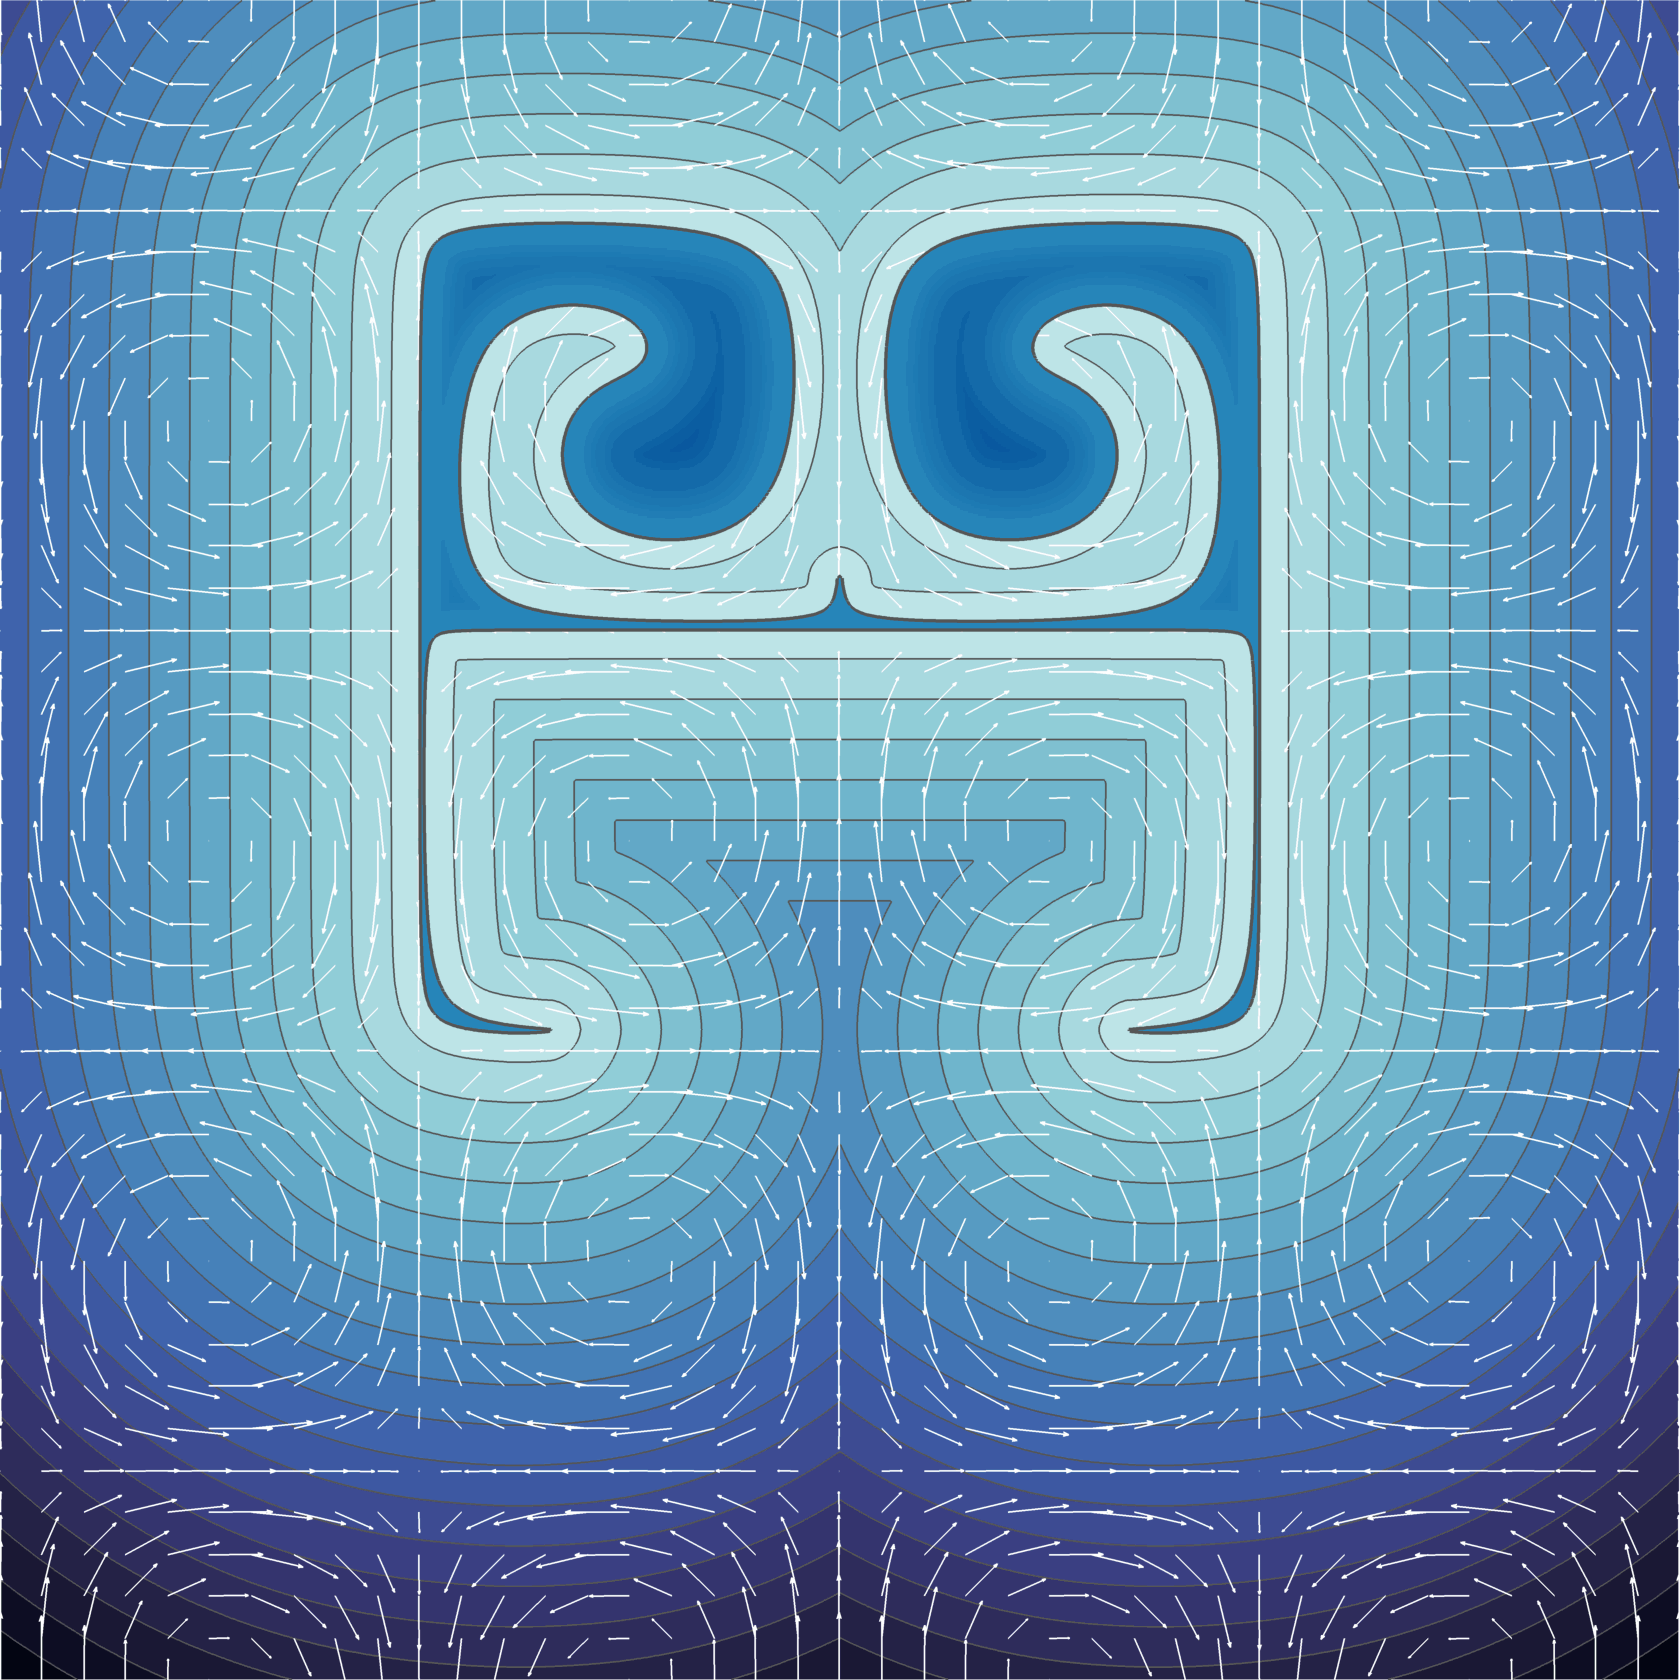
\includegraphics[width=0.6\linewidth]{figure/cover2.png}
\end{figure}

\footnote{封面图片为该求解器计算的一个标准算例\cite{rider_stretching_1995},网格量$1024^2$}

\newpage
\tableofcontents
% titlepage end

% part 2
\newpage
\pagenumbering{arabic}
\setcounter{page}{1}
\section{Level Set方法}
\subsection{基本思想:隐式界面}
Level Set方法的基本思想在于,对于空间中某个界面,我们总可以找到一个函数,使得它在界面一侧值总为正,而在另一侧值总为负。那么该函数的零值面恰好就是所考察界面的一种隐式表达。比起VOF方法,Level Set具有更为清晰的数学描述,且当构造出的隐式界面函数具有很好的性质时,我们可以计算得到光滑的界面曲率,这对于界面-流场间的耦合(表面张力计算)是很有帮助的。

\subsection{界面描述:符号距离函数}
首先我们定义(欧式)\textbf{距离函数(distance function)}:
\begin{equation}
    d(\bm{x})=\min\left(\left|\bm{x}-\bm{x}_I\right|\right)\quad\text{for all}\quad \bm{x}_I\in\partial\Omega
\end{equation}
显然$d(\bm{x})\geq0$,且其梯度的模在除某些奇异点外均为$1$,具有很好的光滑性:
\begin{eqnarray}
    \left|\nabla d\right| &=& \sqrt{\left[\frac{\partial}{\partial x_i}\sqrt{\left(x_l-x_{I,l}\right)\left(x_l-x_{I,l}\right)}\right]\left[\frac{\partial}{\partial x_i}\sqrt{\left(x_l-x_{I,l}\right)\left(x_l-x_{I,l}\right)}\right]}\notag\\
    &=&\sqrt{\frac{1}{2}\frac{2\left(x_i-x_{I,i}\right)}{\sqrt{\left(x_l-x_{I,l}\right)\left(x_l-x_{I,l}\right)}}\cdot\frac{1}{2}\frac{2\left(x_i-x_{I,i}\right)}{\sqrt{\left(x_l-x_{I,l}\right)\left(x_l-x_{I,l}\right)}}}\notag\\
    &=&\sqrt{\frac{\left(x_i-x_{I,i}\right)\left(x_i-x_{I,i}\right)}{\left(x_l-x_{I,l}\right)\left(x_l-x_{I,l}\right)}}\notag\\
    &=&1
\end{eqnarray}
上式采用了爱因斯坦求和约定。

在此基础上定义\textbf{符号距离函数(signed distance function)}$\phi(\bm{x})$,使得$|\phi(\bm{x})|=d(\bm{x})$,并要求它满足隐式界面的定义,具体表达式如下:
\begin{eqnarray}
    \phi(\bm{x})=\left\{\begin{array}{rl}
        d(\bm{x})   & \text{for all}\ \bm{x}\in\Omega^+       \\
        d(\bm{x})=0 & \text{for all}\ \bm{x}\in\partial\Omega \\
        -d(\bm{x})  & \text{for all}\ \bm{x}\in\Omega^-       \\
    \end{array}\right.
    \label{eqn:sdf}
\end{eqnarray}
选取符号距离函数作为隐式界面函数具有十分优良的性质,例如其在界面附近的光滑性,及常梯度幅值$\left|\phi(\bm{x})\right|=1$对于界面曲率计算的大大简化:
\begin{equation}
    \kappa\equiv\nabla\cdot\bm{n}=\nabla^2\phi,\quad \bm{n}=\nabla\phi
\end{equation}

\subsection{界面推进}
自由界面问题中,通常假设两相界面为一物质面,隐式界面函数(这里也就是符号距离函数)$\phi(\bm{x})$的物质导数为零即可得到其演化方程:
\begin{equation}
    \frac{\mathrm{D}\phi}{\mathrm{D}t}=\frac{\partial\phi}{\partial t}+\bm{u}\cdot\nabla\phi=0\quad\text{for all }\bm{x}\in\partial\Omega
    \label{eqn:evolution}
\end{equation}
其中$\bm{u}(x,t)$为界面处流场速度,注意该式理论上仅在界面位置(即$\bm{x}_I:\phi(\bm{x}_I)=0$)成立。

\subsubsection{时间推进}
数值求解\autoref{eqn:evolution}时,时间推进的最简单实现莫过于一阶精度的显式格式——\textbf{前向欧拉方法(forward Euler method)},如下式:
\begin{equation}
    \frac{\phi^{n+1}-\phi^n}{\Delta t}+\bm{u}^n\cdot\nabla\phi^n=0
\end{equation}
其中上标表所处时间步。

考虑进一步提高时间精度,可以采用\textbf{TVD RK(total variation diminishing Runge-Kutta)格式},其二阶精度版本等同于常规RK2格式:
\begin{eqnarray}
    \frac{\phi^{n+1}-\phi^n}{\Delta t}+\bm{u}^n\cdot\nabla\phi^n=0 \\
    \frac{\phi^{n+2}-\phi^{n+1}}{\Delta t}+\bm{u}^{n+1}\cdot\nabla\phi^{n+1}=0 \\
    \phi^{n+1}=\frac{1}{2}\left(\phi^n+\phi^{n+2}\right)
\end{eqnarray}

三阶精度的TVD RK格式如下:
\begin{eqnarray}
    \frac{\phi^{n+1}-\phi^n}{\Delta t}+\bm{u}^n\cdot\nabla\phi^n=0 \\
    \frac{\phi^{n+2}-\phi^{n+1}}{\Delta t}+\bm{u}^{n+1}\cdot\nabla\phi^{n+1}=0 \\
    \phi^{n+\frac{1}{2}}=\frac{3}{4}\phi^n+\frac{1}{4}\phi^{n+2} \\
    \frac{\phi^{n+\frac{3}{2}}-\phi^{n+\frac{1}{2}}}{\Delta t}+\bm{u}^{n+\frac{1}{2}}\cdot\nabla\phi^{n+\frac{1}{2}}=0 \\
    \phi^{n+1}=\frac{1}{3}\phi^{n}+\frac{2}{3}\phi^{n+\frac{3}{2}}
\end{eqnarray}
更高阶的时间推进格式对于提升界面捕捉的时间精度收效甚微(事实上对于自由界面数值解问题,空间离散的精度要求较之时间离散更为重要\citep{osher_level_2003}),上述三种格式通常已经足够。

\subsubsection{空间离散}
在考虑空间离散格式时,我们需要注意到界面演化方程为一对流方程(或称输运方程),它属于双曲型PDE。由于这类方程具有特征线的概念,采用\textbf{迎风格式}进行离散既能满足物理特征,又能保证数值稳定性。

一种简单而具有足够精度的实现方法是采用\textbf{QUICK(quadratic upstream interpolation for convective kinetics)格式}对符号距离函数对流项进行离散,QUICK具有三阶精度。其形式如下:
\begin{equation}
    \phi_w=\frac{1}{8}\left(3\phi_P+6\phi_{W}-\phi_{WW}\right),\quad \text{when }u_x>0
\end{equation}
下标表示空间中各点(见\autoref{fig:gridfvm})。

\begin{figure}[htbp]
    \centering
    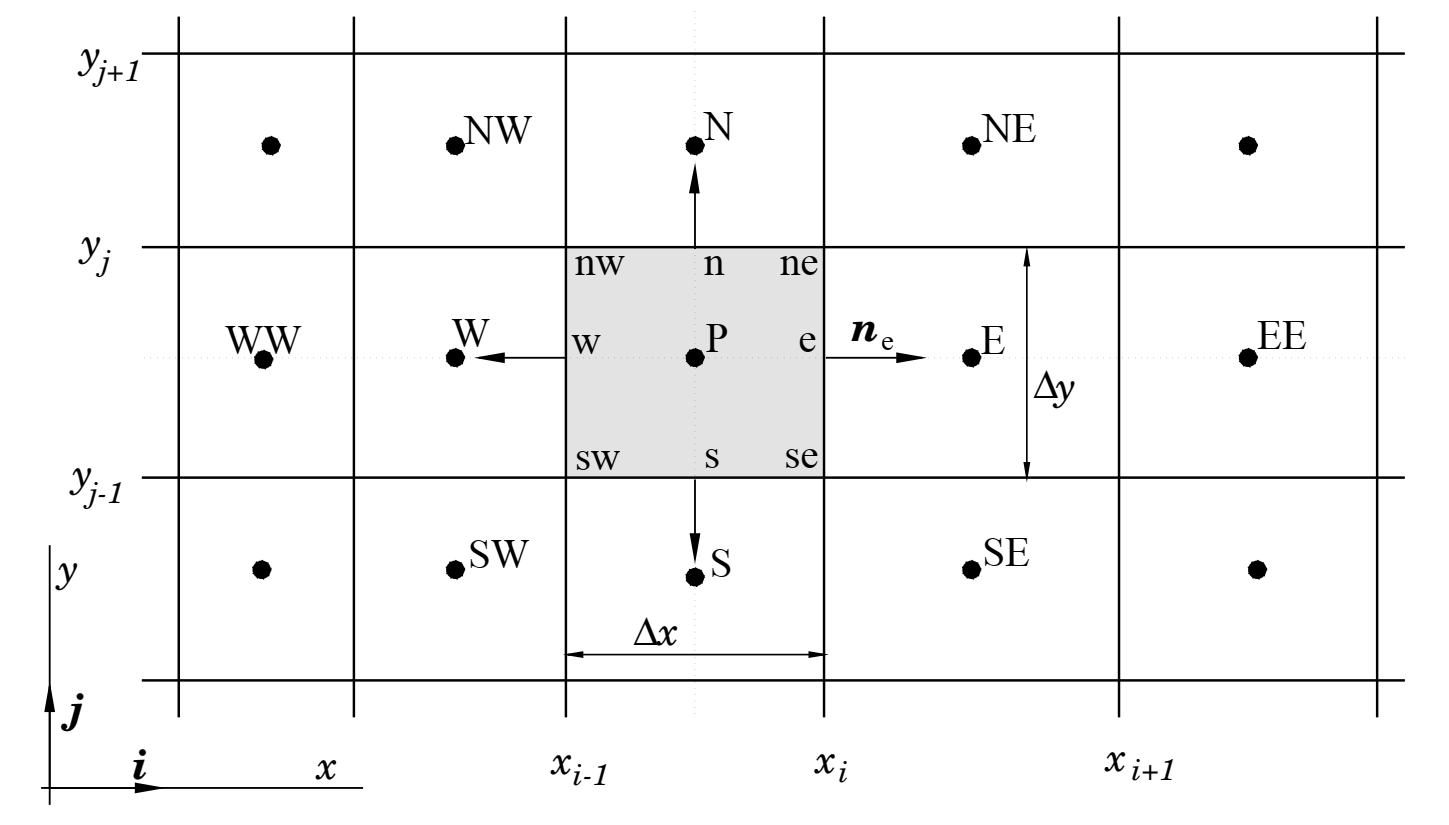
\includegraphics[width=0.6\linewidth]{figure/gridfvm.png}
    \caption{\label{fig:gridfvm}2维笛卡尔网格\citep{ferziger_computational_2020}}
\end{figure}

这里我们实际上使用了有限体积方法求解,注意到界面演化方程(\autoref{eqn:evolution})在不可压条件下可以改写为守恒型:
\begin{eqnarray}
    \frac{\partial \phi}{\partial t}+\nabla\cdot\left(\bm{u}\phi\right)&=&0 \\
    \int_\Omega \frac{\phi^{n+1}-\phi^n}{\Delta t}\ \mathrm{d}\Omega+\int_{\partial\Omega}\phi\bm{u}\cdot\bm{n}\ \mathrm{d}S&=&0 \\
    \Longrightarrow \frac{\phi^{n+1}_{i,j}-\phi^n_{i,j}}{\Delta t}+\frac{\left(u_{i+\frac{1}{2},j}\phi_{i+\frac{1}{2},j}-u_{i-\frac{1}{2},j}\phi_{i-\frac{1}{2},j}\right)}{h} & & \notag\\+\frac{\left(u_{i,j +\frac{1}{2}}\phi_{i,j+\frac{1}{2}}-u_{i,j-\frac{1}{2}}\phi_{i,j-\frac{1}{2}}\right)}{h}&=&0
\end{eqnarray}
其中控制体表面中点插值采用前述QUICK格式实现。

\subsection{符号距离函数计算}
\subsubsection{首次初始化}
几何界面初始化时,可以先依据各几何单元性质计算其距离函数分布,以\autoref{subsec:rotation}中缺角圆盘首次初始化为例。把缺角圆盘边界分解为1个圆弧段、2条线段、3个点共6个基本几何单元。点对距离函数的贡献为以该点为中心辐射出的同心圆,记$d_{p}(\bm{x}),\bm{x}\in\Omega$;直线段对距离函数的贡献在过其两端点,垂直于该线段的直线之间的区域内,值等于到线段的垂直距离$d_{l}(\bm{x}),\bm{x}\in\Omega_l$;圆弧段对距离函数的贡献在该圆弧对应的夹角范围之内的区域,等高线呈同心圆分布$d_{c}(\bm{x}),\bm{x}\in\Omega_c$。于是距离函数可以表示为:
\begin{equation}
    d(\bm{x})=\min\left\{
    d_{p_i}(\bm{x}),d_{l_j}(\bm{x}),d_{c_k}(\bm{x})
    \right\},\quad \bm{x}\in\Omega\cap\Omega_l\cap\Omega_c
\end{equation}
*这里表达式不太清楚,总之核心思想是在各单元的作用区间上任一点,选取到所有有贡献单元的距离的最小值,具体实现见代码中缺角圆盘的初始化过程。

\subsubsection{重新初始化}
在建立界面模型时,我们假设两侧物质不发生蒸发、凝结、渗透或相互溶解,进而可以认为两相界面为一物质面,得到其演化方程。然而在数值求解时,我们对全场均按照界面方程推进,使得远离界面位置的$\phi$偏离了“符号距离函数”这一定义。这种偏离将会导致两个问题\citep{prosperetti_computational_2009}:
\begin{enumerate}
    \item 界面附近梯度$|\nabla\phi|$可能极小或极大,影响界面演化方程离散求解的精度;
    \item 在与流场控制方程耦合时,表面曲率-张力的计算借用了符号距离函数梯度模为1的性质,如若偏离则会破坏该条件,进而导致耦合计算错误。
\end{enumerate}
为此,在界面推进时周期性地将$\phi$重新初始化为正确的符号距离函数是非常有必要的,\textbf{重新初始化(reinitialization)}过程一般通过求解下述方程实现:
\begin{equation}
    \frac{\partial \phi}{\partial \tau}=S(\phi^0)\left(1-|\nabla\phi|\right)
    \label{eqn:reinit}
\end{equation}
其中$\tau$表示伪时间,容易看到上式意味着:
\begin{eqnarray}
    \frac{\partial \phi}{\partial \tau}=0\Longleftrightarrow\left\{\begin{array}{l}
        |\nabla\phi|=1 \\
        S(\phi^0)=0\Longleftrightarrow\phi^0(\bm{x}_I)=0
    \end{array}\right.
\end{eqnarray}
其中$S(\cdot)$为\textbf{sharp sign function},其定义并不唯一。

\citet{sussman_level_1994}给出了一种简单可行的重新初始化方法,注意到重新初始化方程(\autoref{eqn:reinit})可以写为对流形式:
\begin{equation}
    \frac{\partial \phi}{\partial t}+S(\phi^0)\frac{\nabla\phi}{|\nabla\phi|}\cdot\nabla\phi=S(\phi^0)
\end{equation}
其中$\bm{v}\equiv S(\phi^0)\frac{\nabla\phi}{|\nabla\phi|}$从界面向外法向辐射,这意味着重新初始化过程中也需要采用迎风格式求解。在伪时间上离散:
\begin{equation}
    \phi^{n+1}_{i,j}=\phi^n_{i,j}-\Delta\tau S_\varepsilon\left(\phi^0_{i,j}\right)G\left(\phi^n_{i,j}\right)
\end{equation}
其中:
\begin{equation}
    S_\varepsilon(\phi_{i,j})\equiv\frac{\phi_{i,j}}{\sqrt{\phi^2_{i,j}+\varepsilon^2}}\notag
\end{equation}
\begin{equation}
    G(\phi^n_{i,j})=\left\{\begin{array}{ll}
        \sqrt{\max\left(a_+^2,b_-^2\right)+\max\left(c_+^2,d_-^2\right)}-1 & \text{if\ \ } \phi^0_{i,j}>0 \\
        \sqrt{\max\left(a_-^2,b_+^2\right)+\max\left(c_-^2,d_+^2\right)}-1 & \text{if\ \ } \phi^0_{i,j}>0 \\
        0                                                                  & \text{otherwise}             \\
    \end{array}\right. \notag
\end{equation}
\begin{eqnarray}
    a &\equiv& D^-_x\phi_{i,j}=\left(\phi_{i,j}-\phi_{i-1,j}\right)/h \notag\\
    b &\equiv& D^+_x\phi_{i,j}=\left(\phi_{i+1,j}-\phi_{i,j}\right)/h \notag\\
    c &\equiv& D^-_y\phi_{i,j}=\left(\phi_{i,j}-\phi_{i,j-1}\right)/h \notag\\
    d &\equiv& D^+_y\phi_{i,j}=\left(\phi_{i,j+1}-\phi_{i,j}\right)/h \notag
\end{eqnarray}
\begin{equation}
    f_+\equiv\max\left(f,0\right),\quad f_-\equiv\min\left(f,0\right) \notag
\end{equation}

虽然该方法仅采用一阶迎风格式离散,但由于符号距离函数本身的光滑性(仅存在一阶导数),所以空间精度是足够的。但仍存在一个关键问题,该方法在邻近界面处实际上并非“迎风”,而是跨过界面传递信息,这将使得界面倾向于移动到最近的网格点上,进一步破坏体积守恒。

为了改进上述方法在邻近界面位置上的缺陷,\citet{russo_remark_2000}提出了\textbf{Reinitialization with subcell fix}方法:
\begin{equation}
    \phi^{n+1}_{i,j}=\left\{\begin{array}{ll}
        \phi^n_{i,j}-\frac{\Delta \tau}{h}\left[\mathrm{sgn}\left(\phi^0_{i,j}\right)|\phi^n_{i,j}|-D_{i,j}\right] & \text{if\ }\left(i,j\right)\in\Sigma_{h} \\
        \phi^n_{i,j}-\Delta\tau\ \mathrm{sgn}\left(\phi^0_{i,j}\right)G\left(\phi^n_{i,j}\right)                   & \text{otherwise}
    \end{array}\right.
\end{equation}
界面邻域$\Sigma_h$定义为:
\begin{equation}
    \left(i,j\right)\in\Sigma_{h}\Longleftrightarrow \phi^0_{i,j}\phi^0_{i\pm1,j\pm1}<0
\end{equation}
$D_{i,j}$表示节点$(i,j)$到界面的实际距离,可以通过下式估计:
\begin{equation}
    D_{i,j}\equiv\frac{h\phi^0_{i,j}}{\Delta\phi^0_{i,j}}
\end{equation}
其中
\begin{eqnarray}
    \Delta\phi^0_{i,j}\equiv\max\bigg\{
    \frac{1}{2}\left[\left(\phi^0_{i+1,j}-\phi^0_{i-1,j}\right)^2+\left(\phi^0_{i,j+1}-\phi^0_{i,j-1}\right)^2\right]^{1/2},\notag\\
    \left|\phi^0_{i+1,j}-\phi^0_{i,j}\right|,\left|\phi^0_{i,j}-\phi^0_{i-1,j}\right|,
    \left|\phi^0_{i,j+1}-\phi^0_{i,j}\right|,\left|\phi^0_{i,j}-\phi^0_{i,j-1}\right|
    \bigg\}
\end{eqnarray}

Subcell fix方法的基本思想就是利用界面附近梯度构造出真实界面位置,避免跨过界面取值,进而可以一定程度上改善\citep{sussman_level_1994}中重新初始化导致体积不守恒的问题。

% part 5
\newpage
\section{算例验证与分析}
\subsection{液滴在剪切流中变形}
\subsubsection{问题描述}
考察圆形液滴在给定剪切流场中的变形情况,流场速度分布如下:
\begin{eqnarray}
    u&=&-2\pi\cos\left[\pi(x-0.5)\right]\sin\left[\pi(y-0.5)\right] \notag\\
    v&=&2\pi\sin\left[\pi(x-0.5)\right]\cos\left[\pi(y-0.5)\right] \notag
\end{eqnarray}
初始时刻($t=0$)液滴半径$r=0.2$,圆心位置:
\begin{equation}
    x_c=0.5,\quad y_c=0.3 \notag
\end{equation}
该问题出自\citep{rider_stretching_1995},作为评估数值格式在剪切流动中界面捕捉效果的一个标准测试。通过流场反转($t_\text{max}=2$,$t=0.5t_\text{max}$时),可以检验数值格式的体积保持特性(理论上应当反演回初始形态)。

\subsubsection{反演}
\autoref{fig:return}展示了网格由疏变密时各种方法的界面演化反演特性,可见不加重新初始化的基础Level Set方法表现最佳,增加重新初始化过程后,$\phi$值分布确实回归到符号距离函数,但并不能非常完整地回归到初始圆形界面。

事实上,\citet{gomez_reinitialization_2005},\citet{hartmann_constrained_2010}均已指出,对于剪切流变形这一算例,网格分辨率对于计算精度有决定性的影响。由于重新初始化过程无法保证液滴变形后尾部尖锐区域得到准确的解析,反而会引入额外的不可逆误差,进而在速度反向后无法完全还原初始状态。前者使用了自适应网格加密(Narrow band and local grid refinement)方法来提升尾部尖锐处解析精度,后者则构造了一类高精度约束重新初始化(high-order constrained reinitialization)方法用以处理这一问题。

\begin{figure}[p]
    \centering
    \footnotesize
    \subfigure[$N=32$, no reinit]{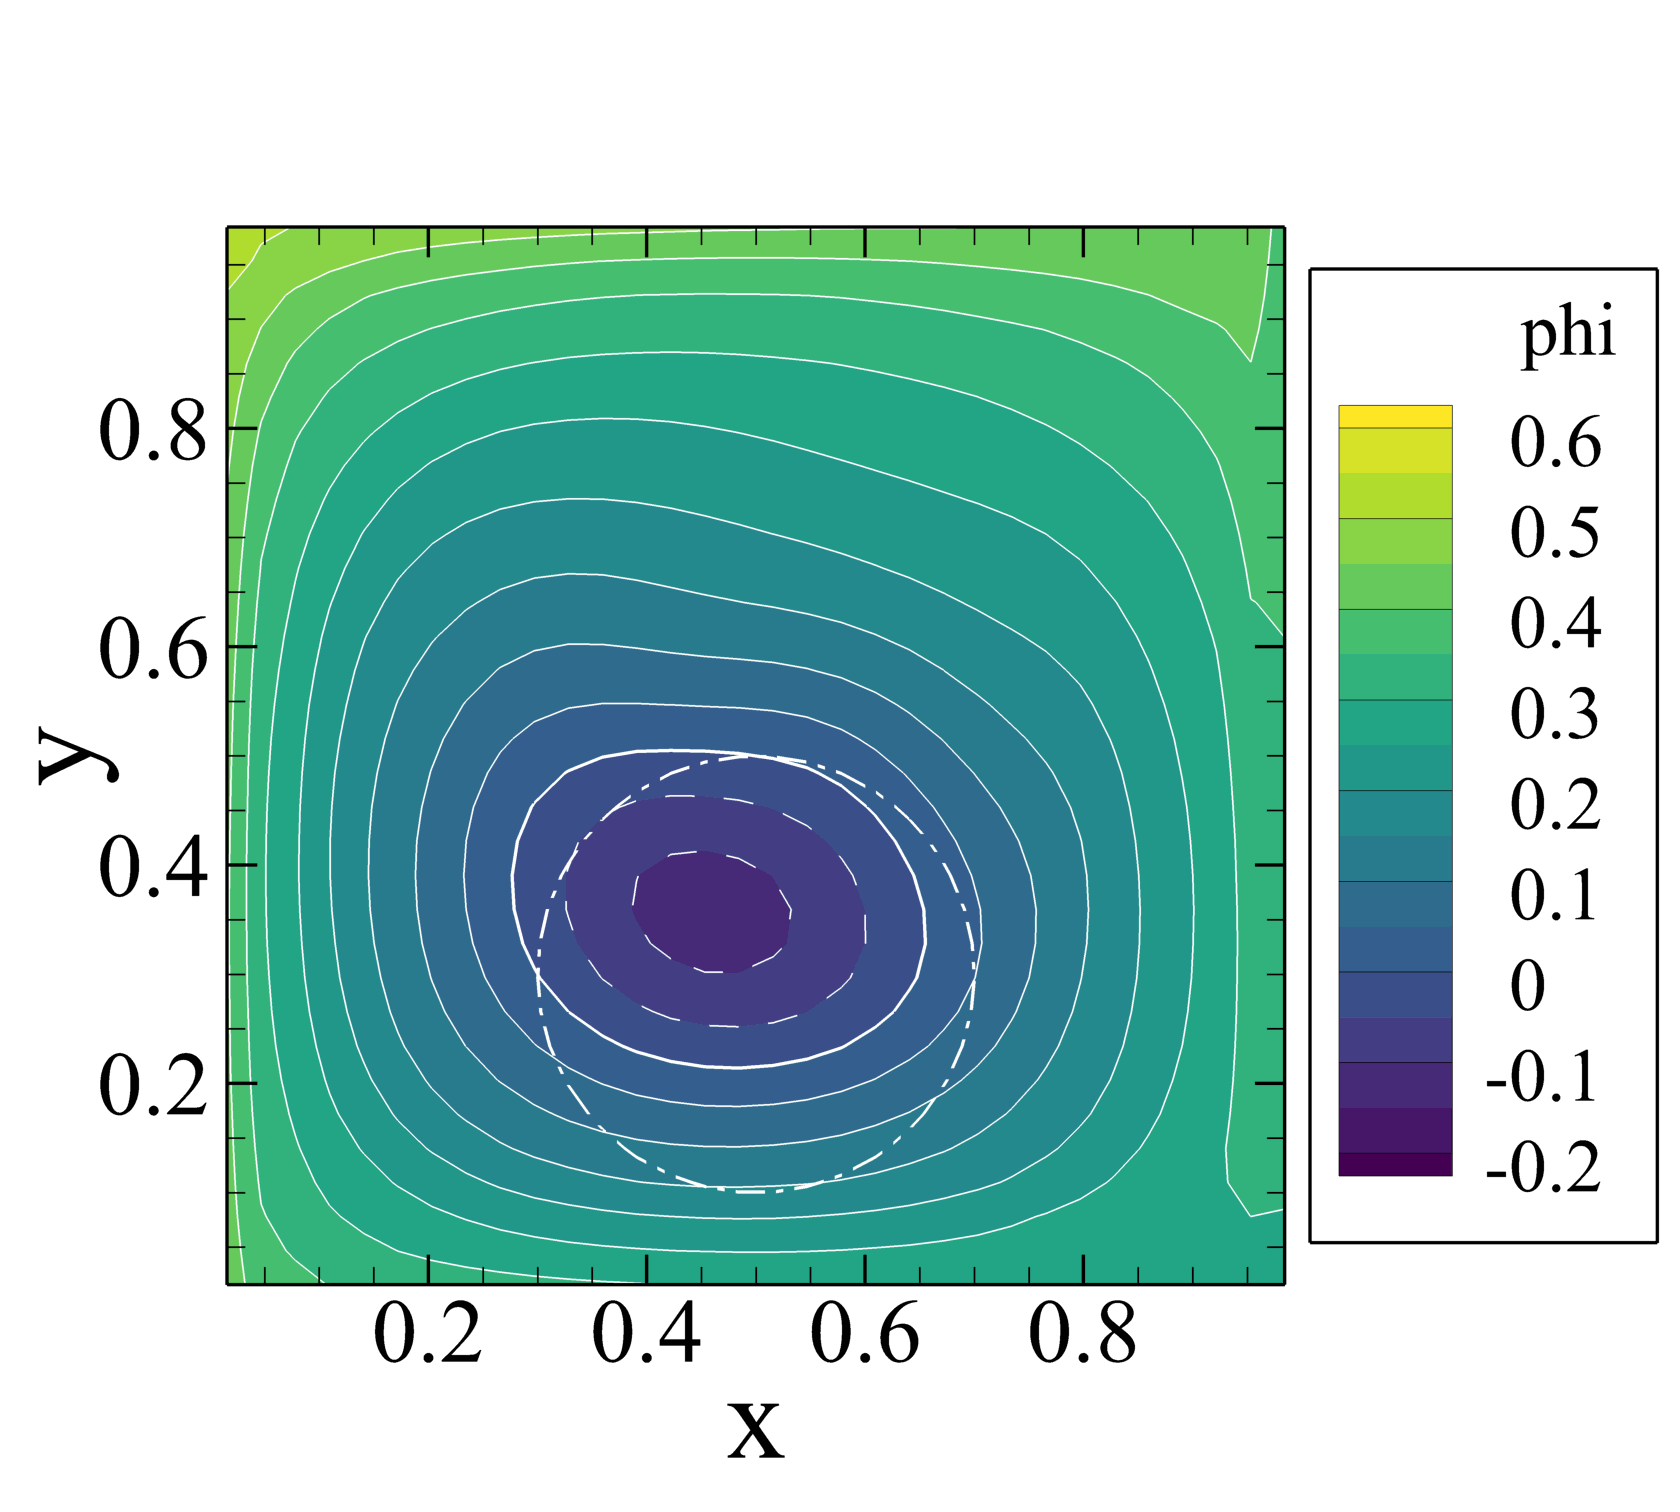
\includegraphics[width=0.24\linewidth]{figure/t2n32r0.png}}
    \subfigure[$N=64$, no reinit]{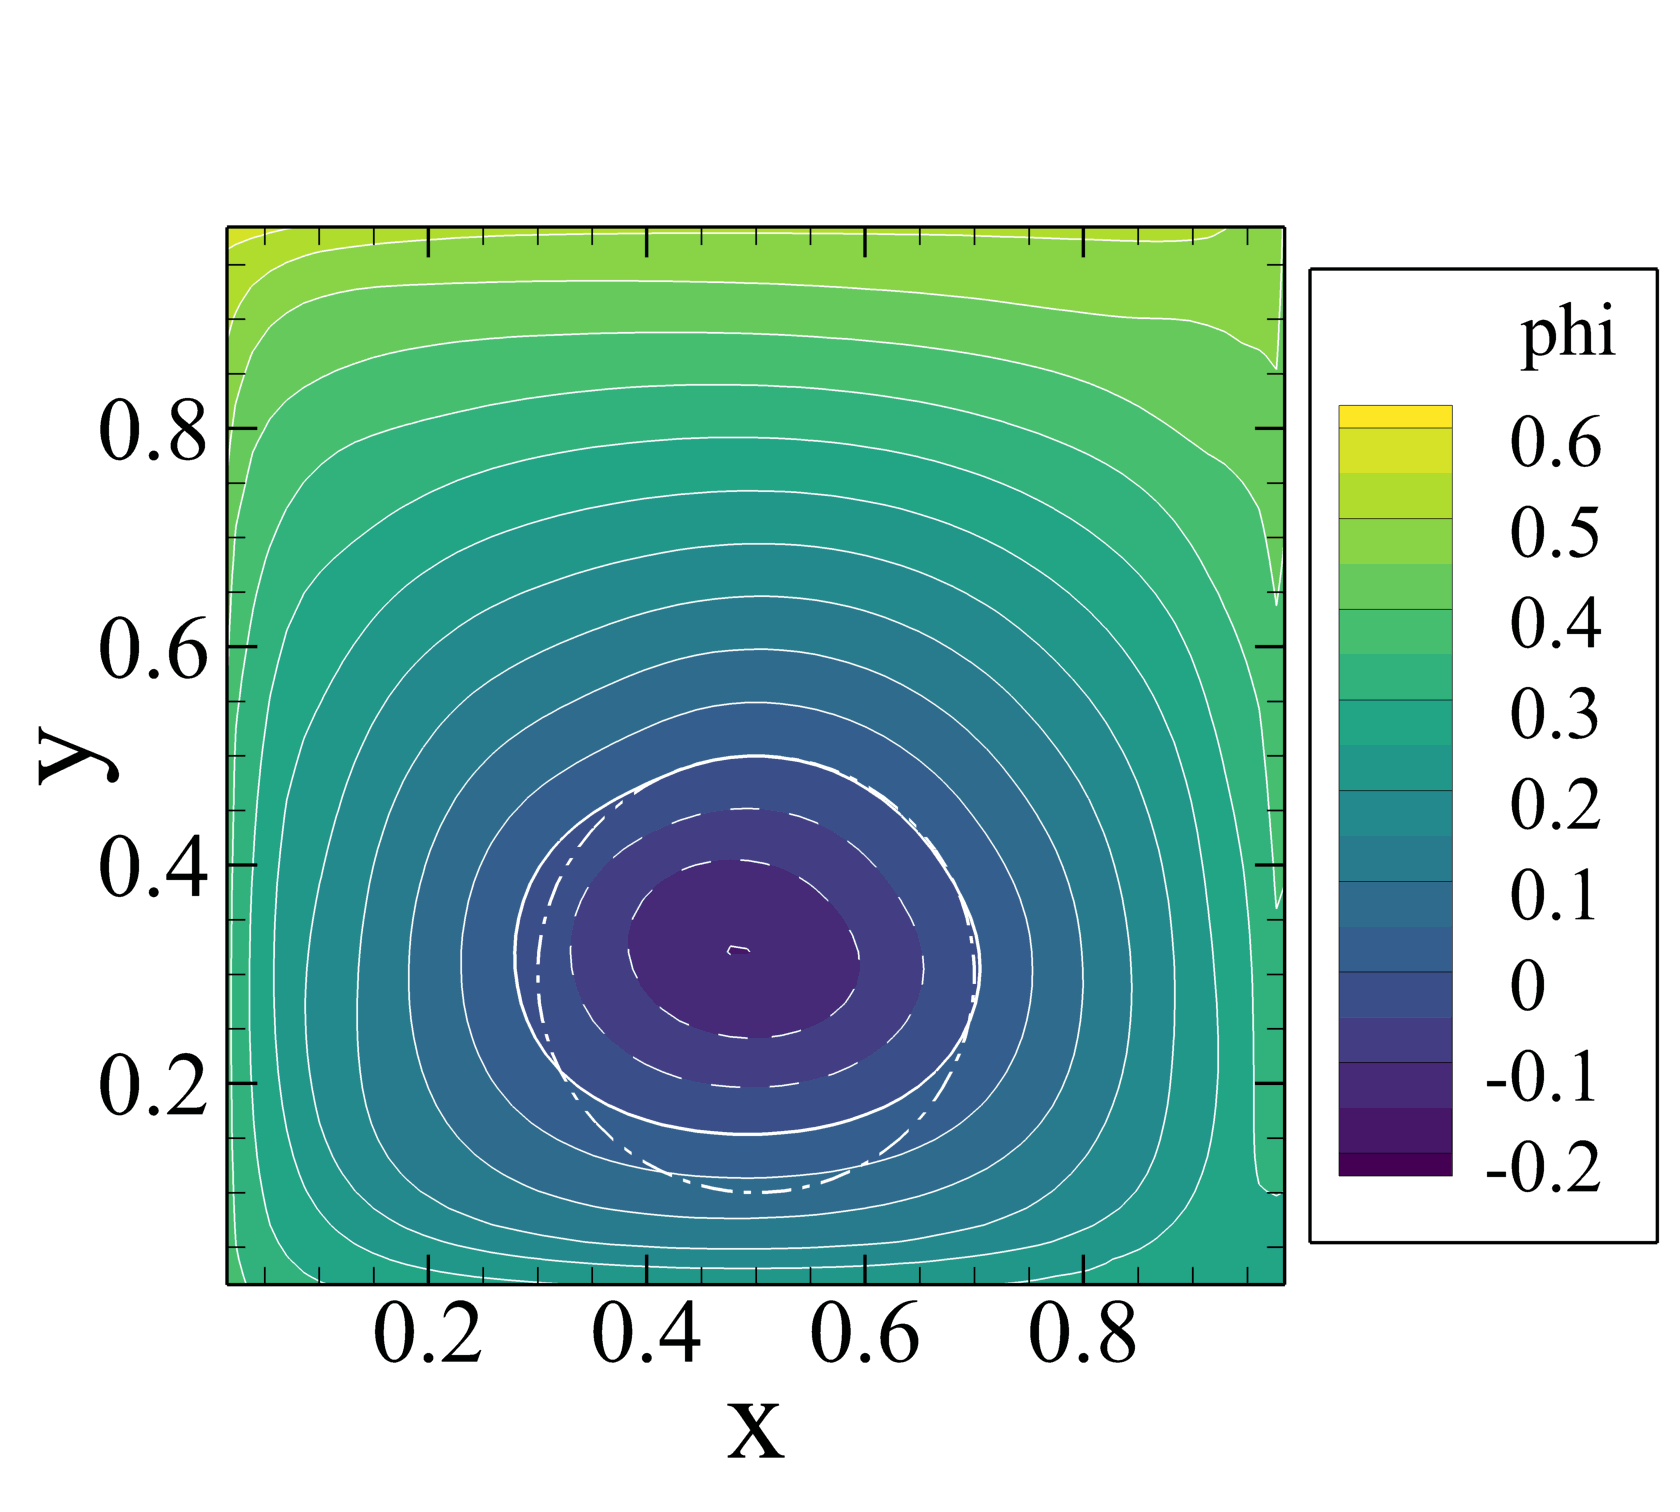
\includegraphics[width=0.24\linewidth]{figure/t2n64r0.png}}
    \subfigure[$N=128$, no reinit]{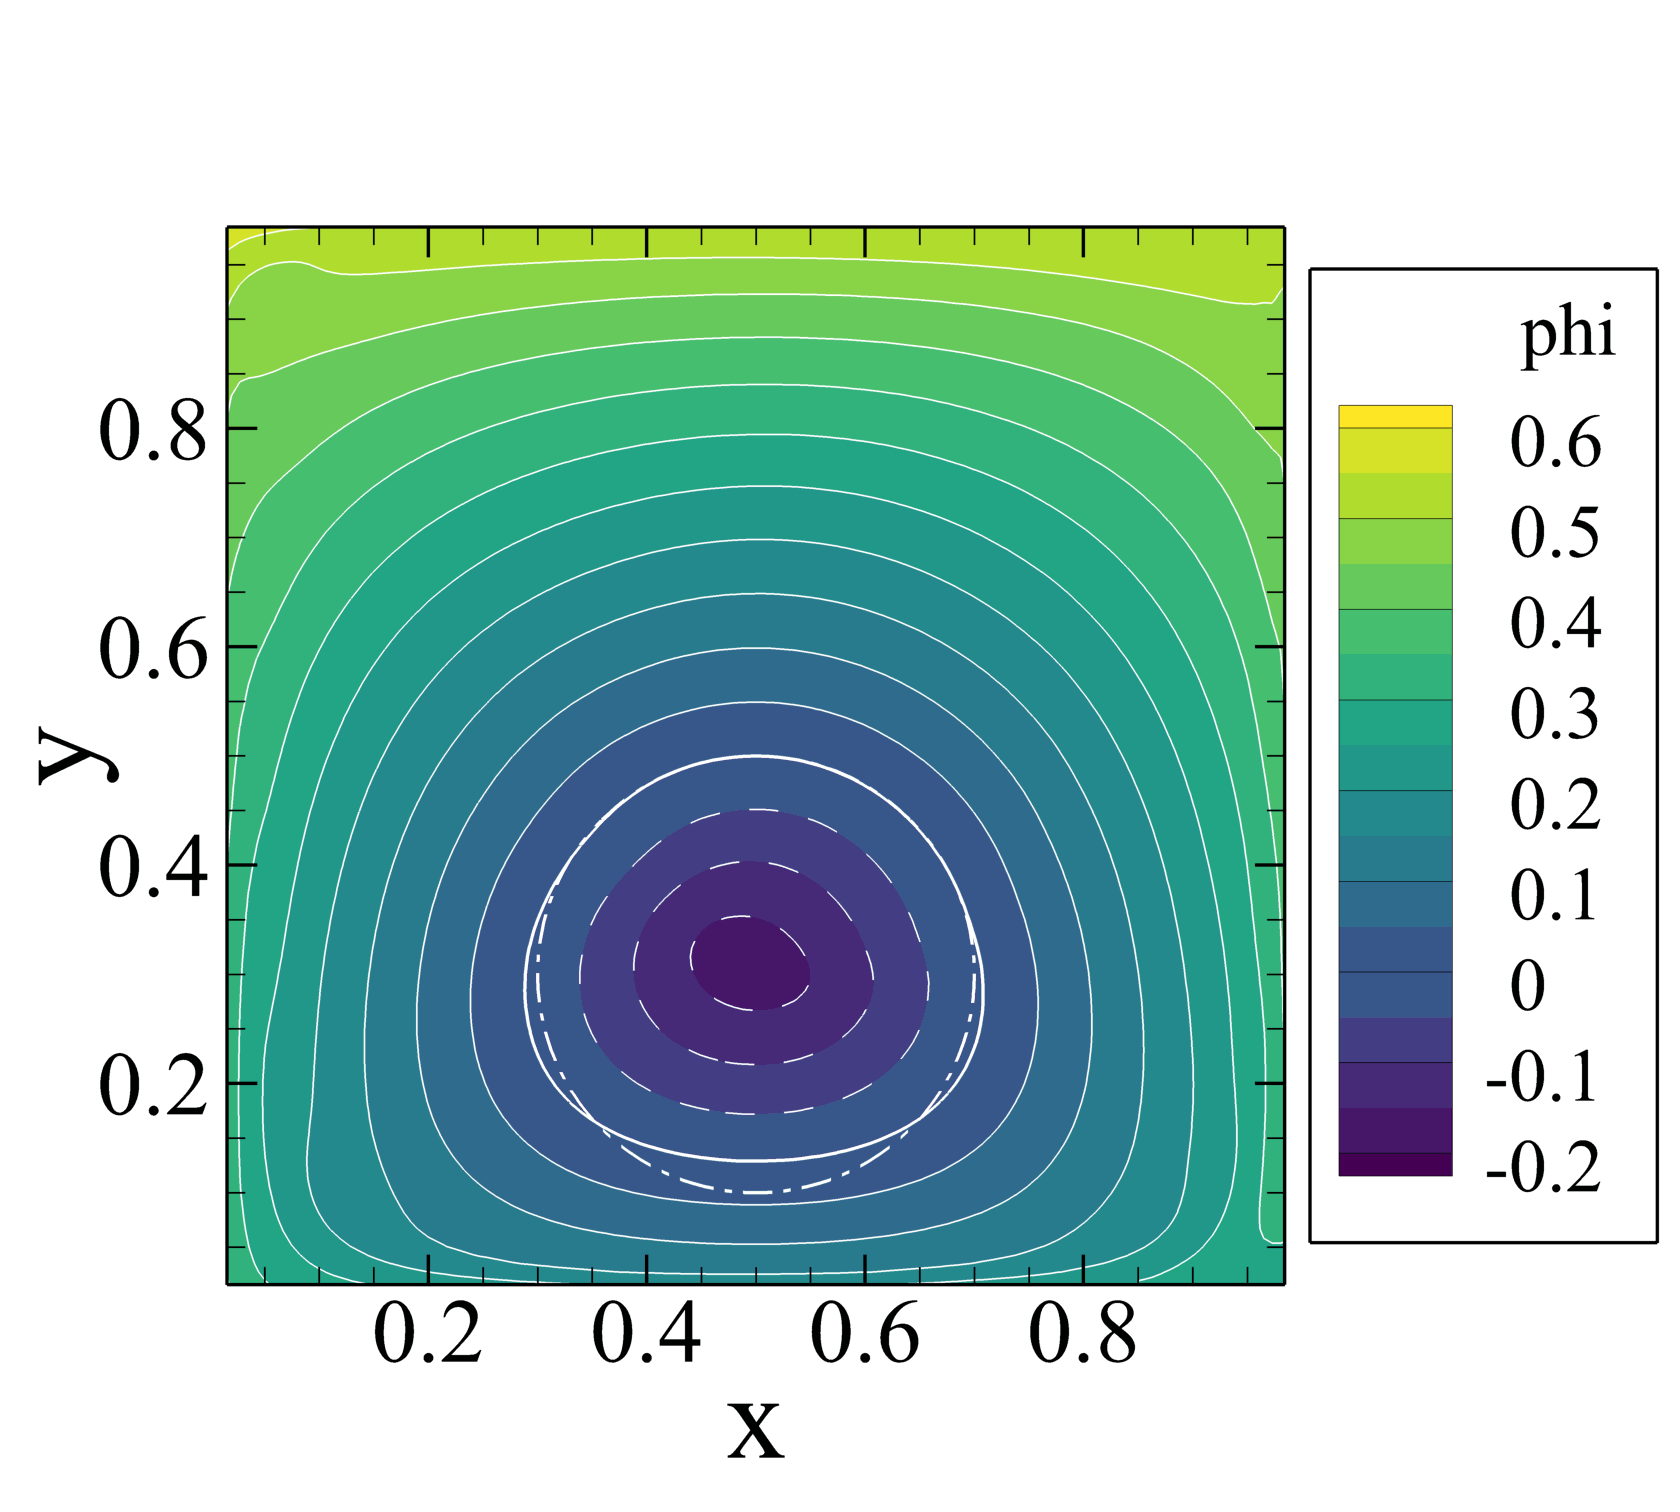
\includegraphics[width=0.24\linewidth]{figure/t2n128r0.png}}
    \subfigure[$N=256$, no reinit]{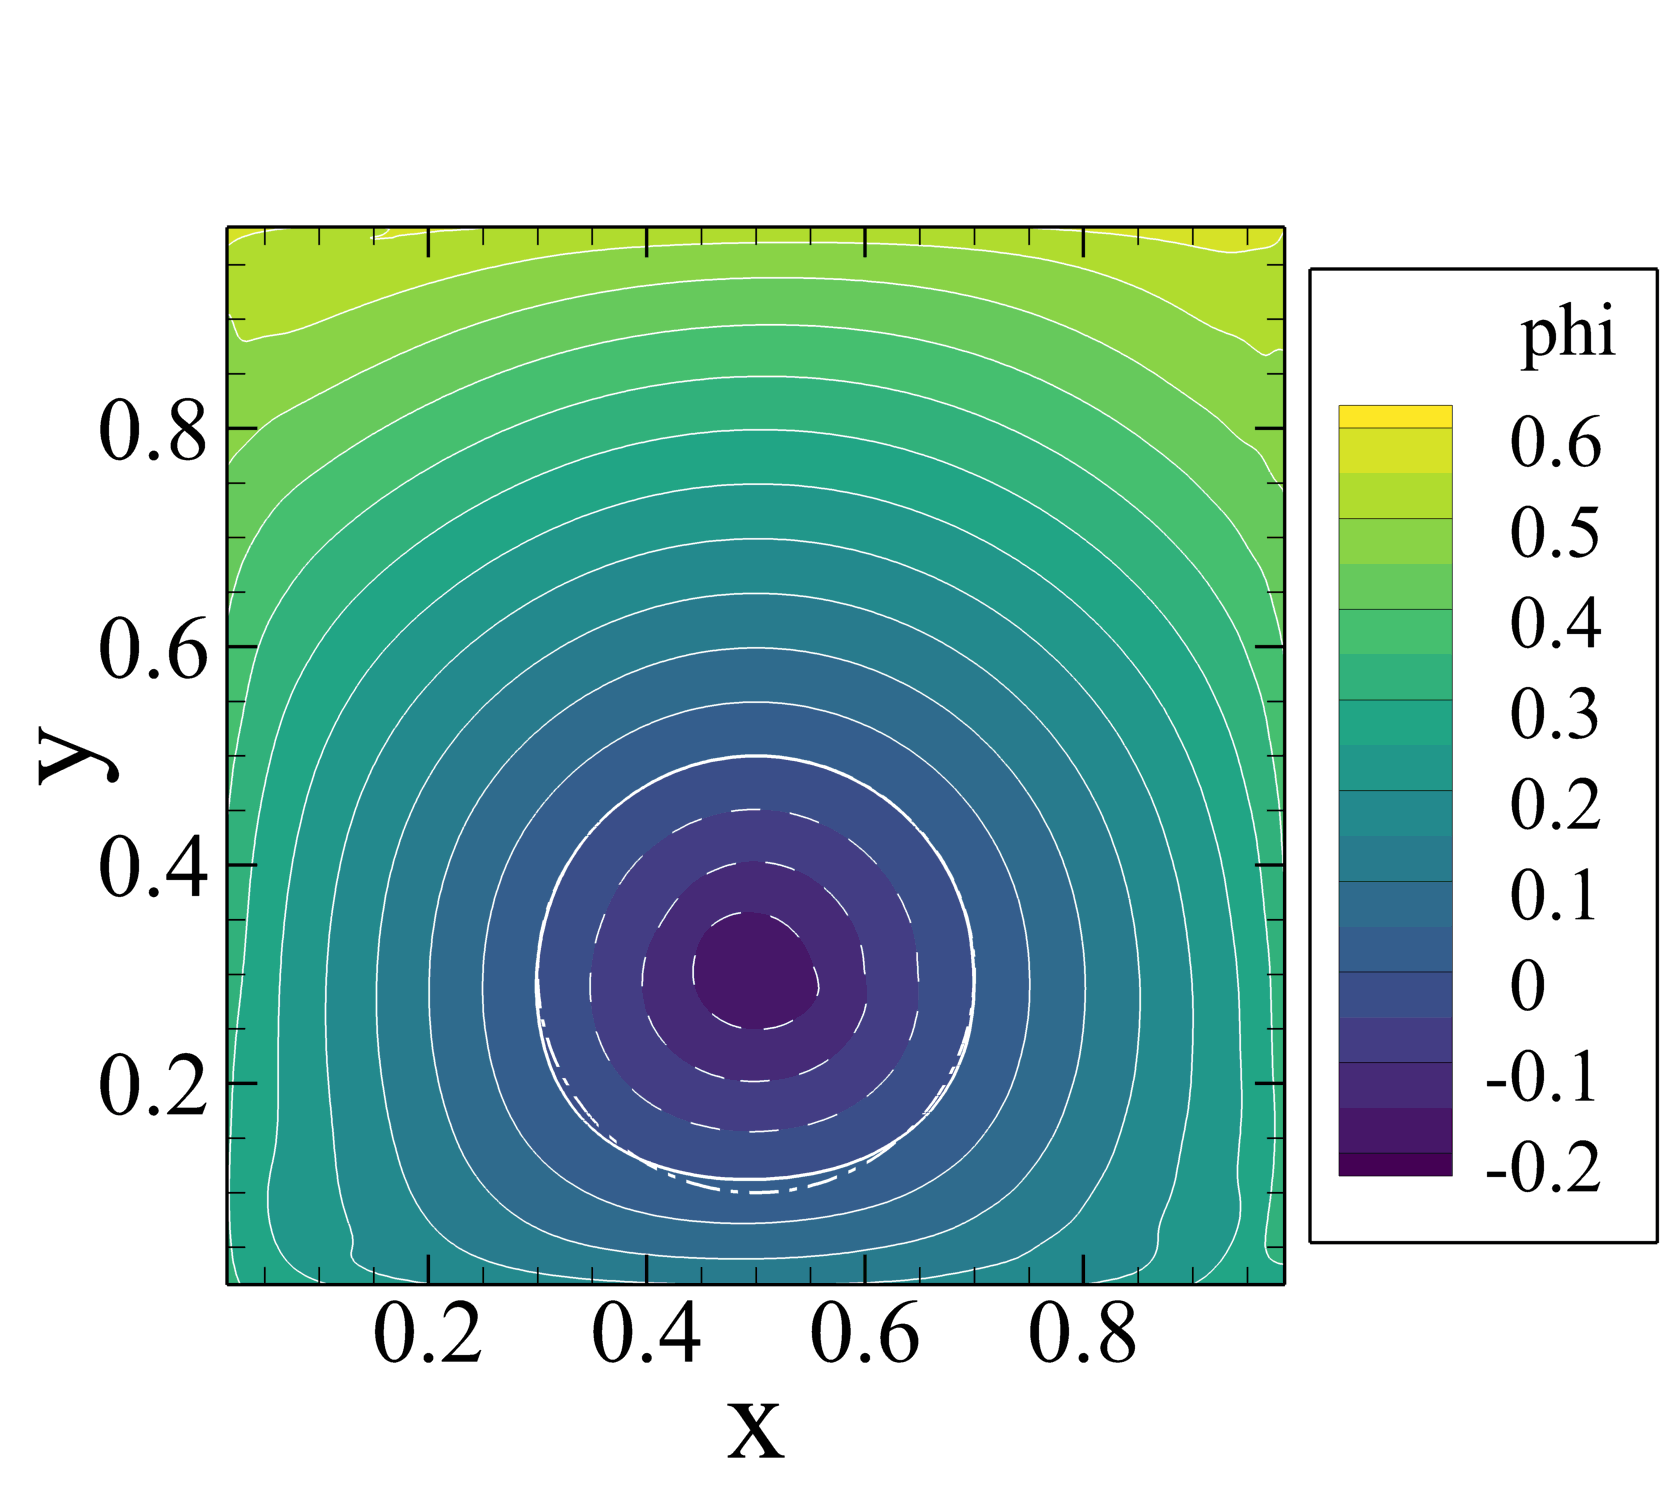
\includegraphics[width=0.24\linewidth]{figure/t2n256r0.png}}
    \subfigure[$N=32$, simple reinit]{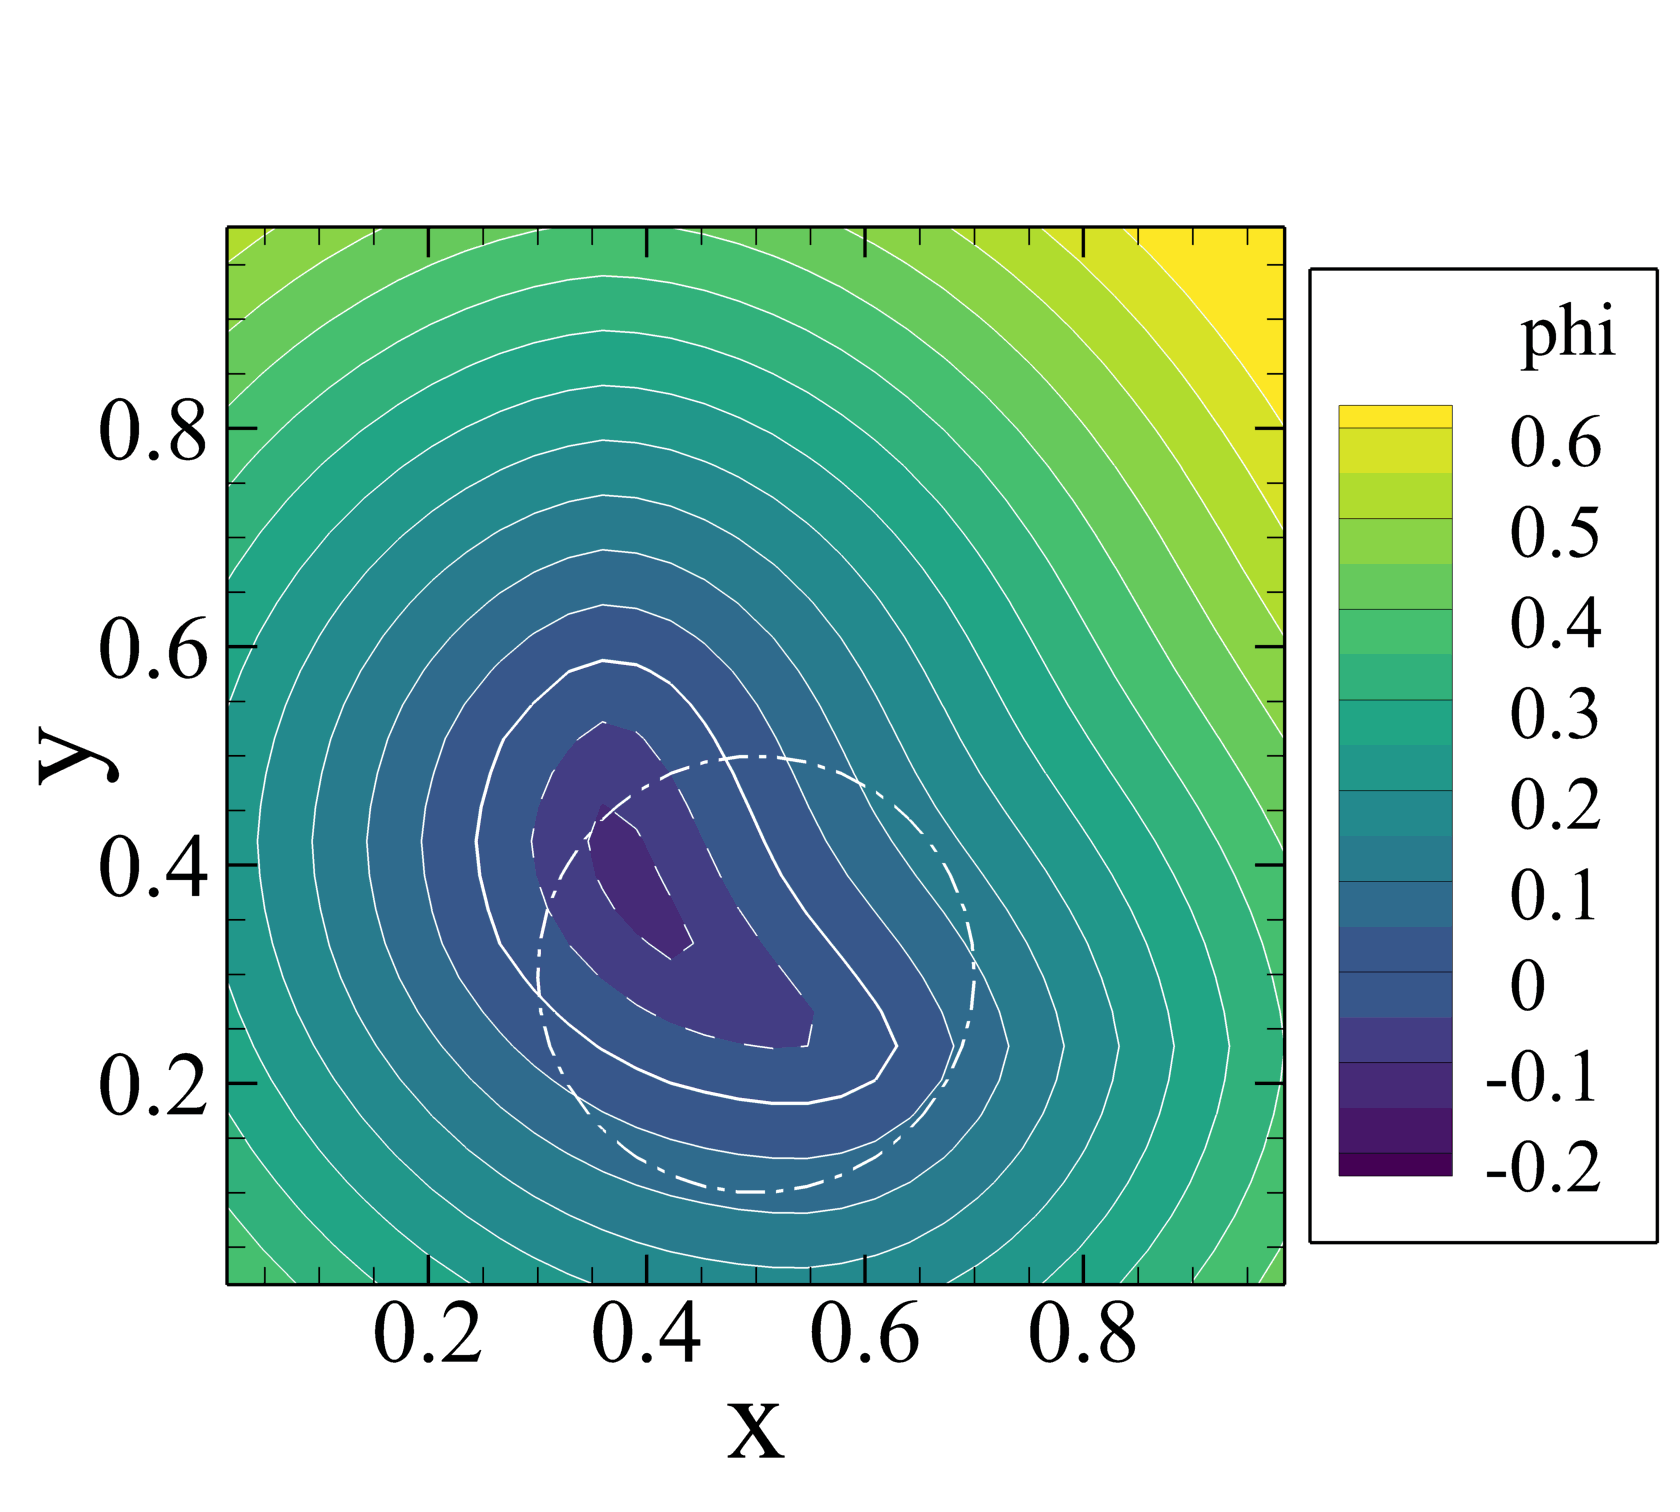
\includegraphics[width=0.24\linewidth]{figure/t2n32r1_2500.png}}
    \subfigure[$N=64$, simple reinit]{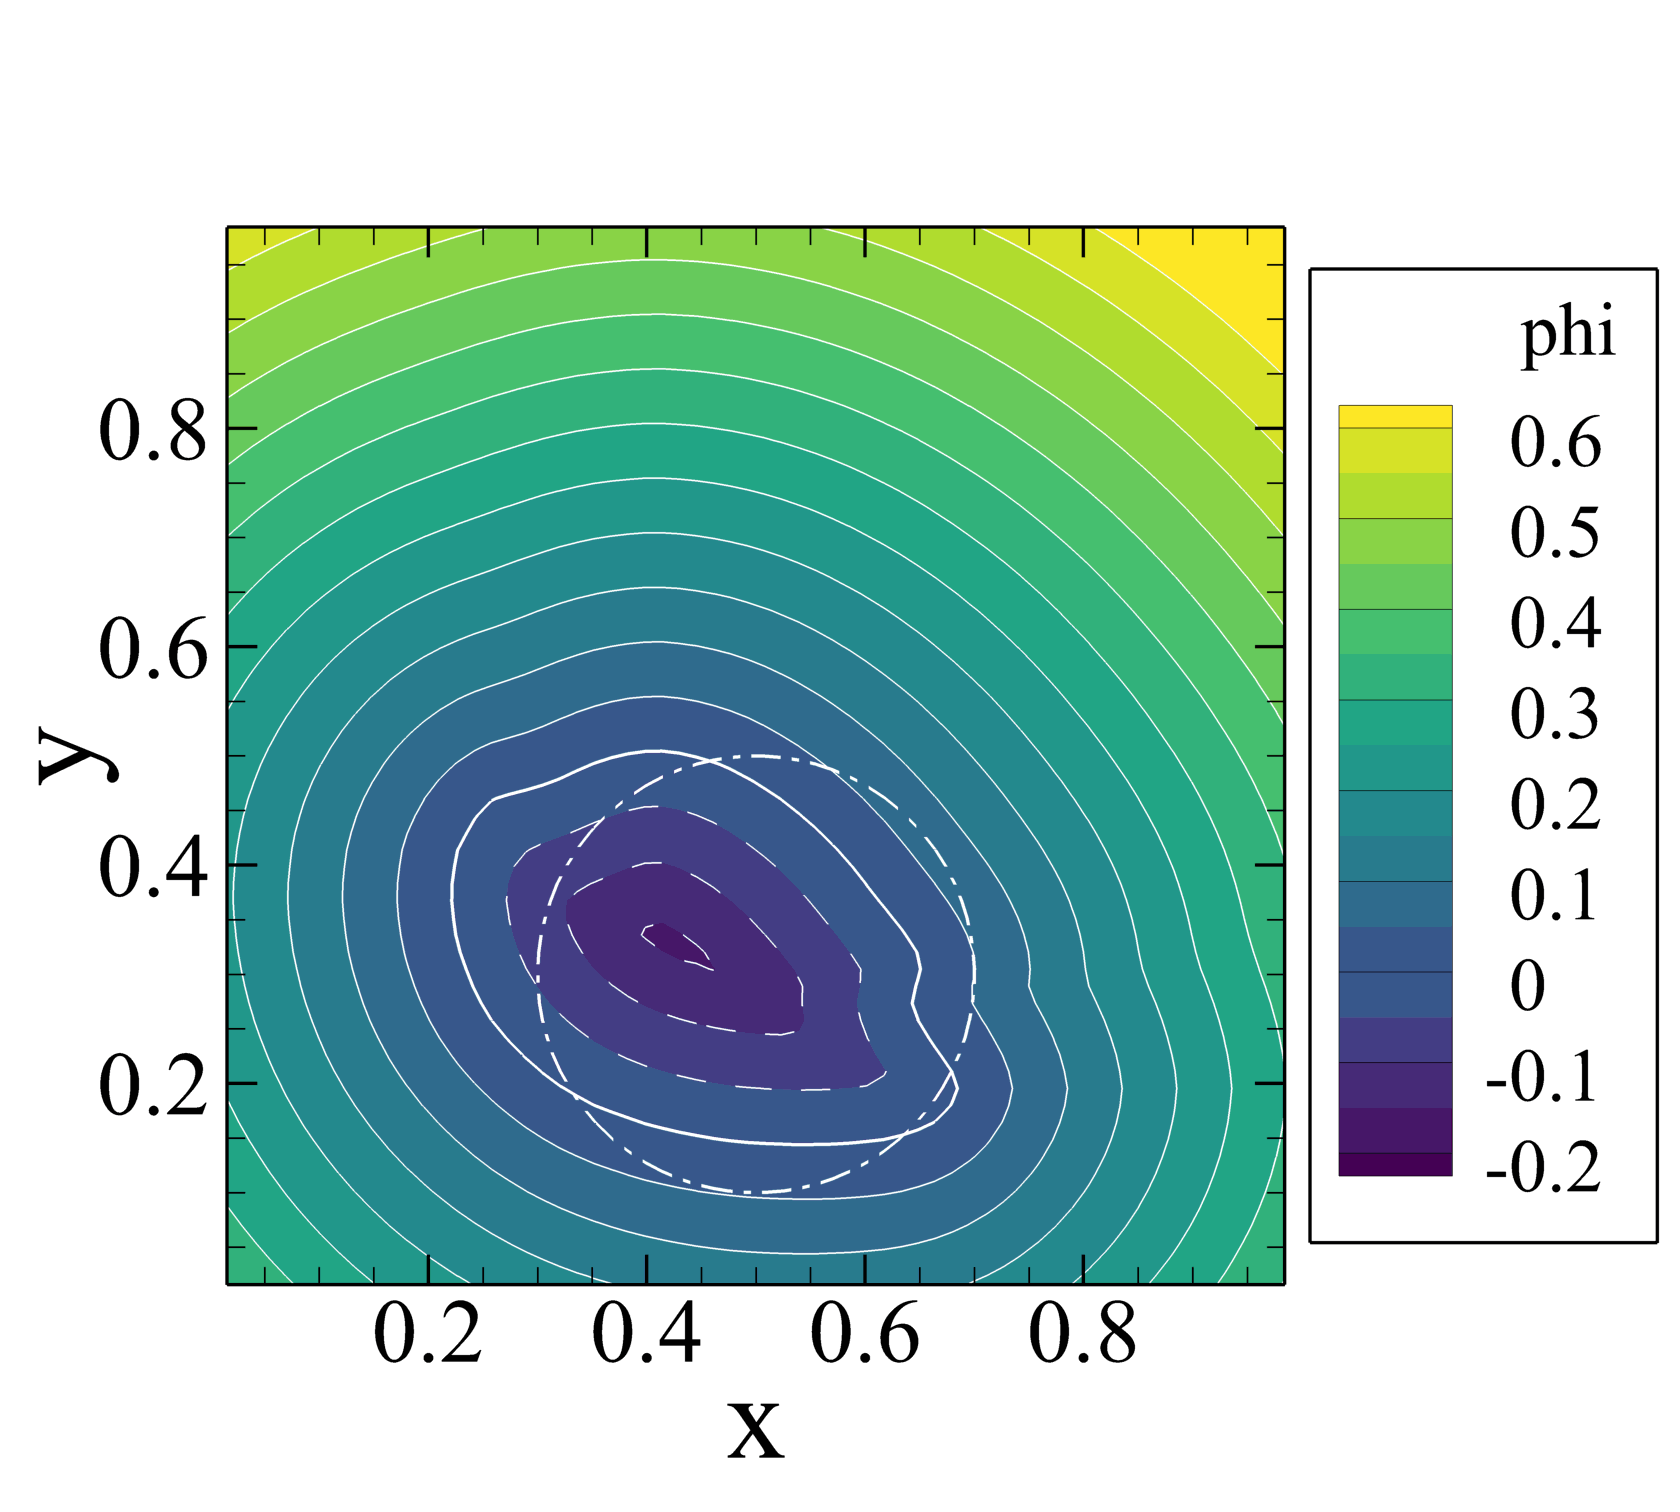
\includegraphics[width=0.24\linewidth]{figure/t2n64r1_2500.png}}
    \subfigure[$N=128$, simple reinit]{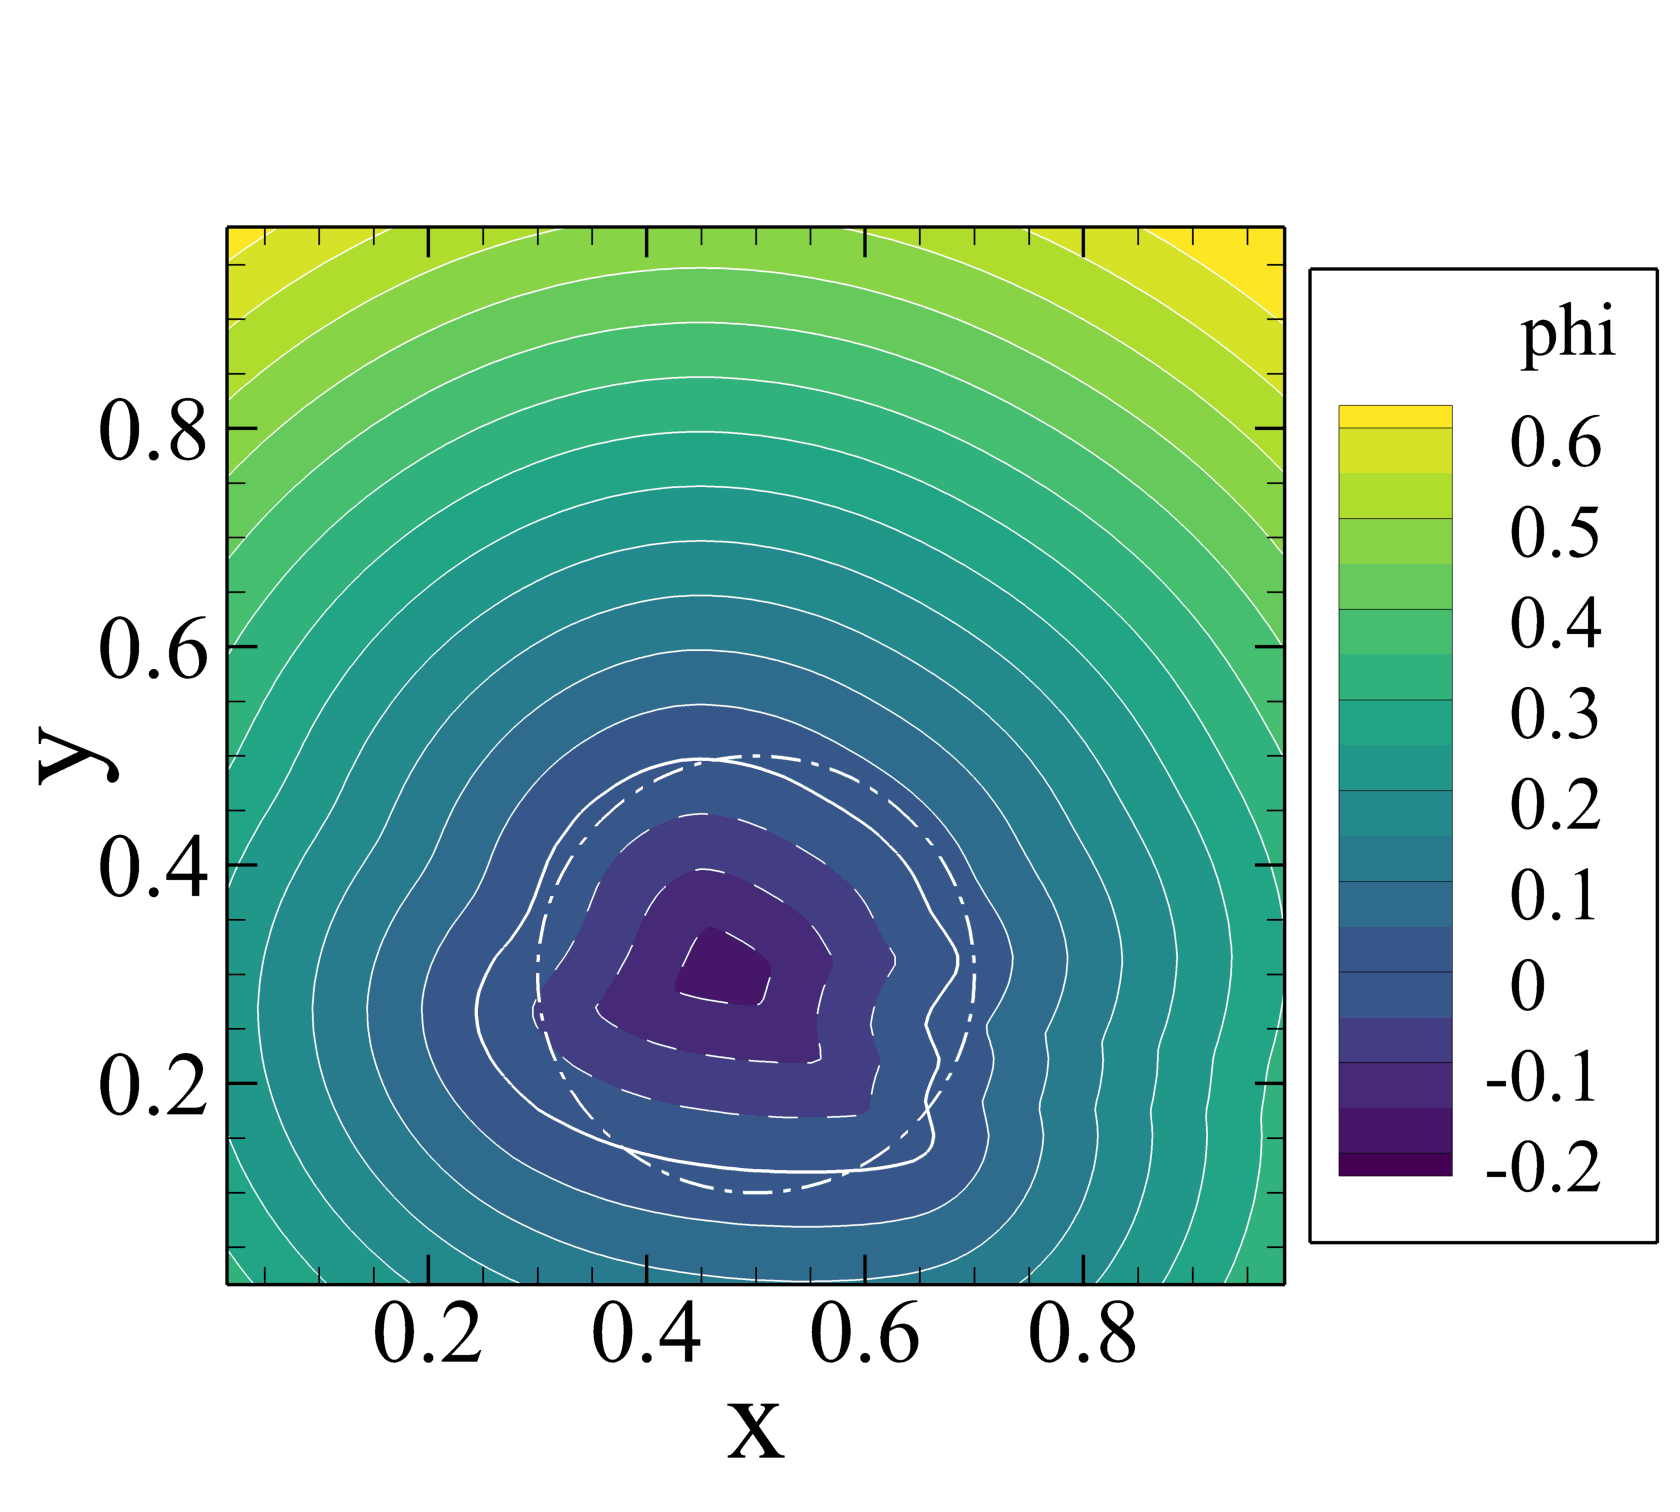
\includegraphics[width=0.24\linewidth]{figure/t2n128r1_2500.png}}
    \subfigure[$N=256$, simple reinit]{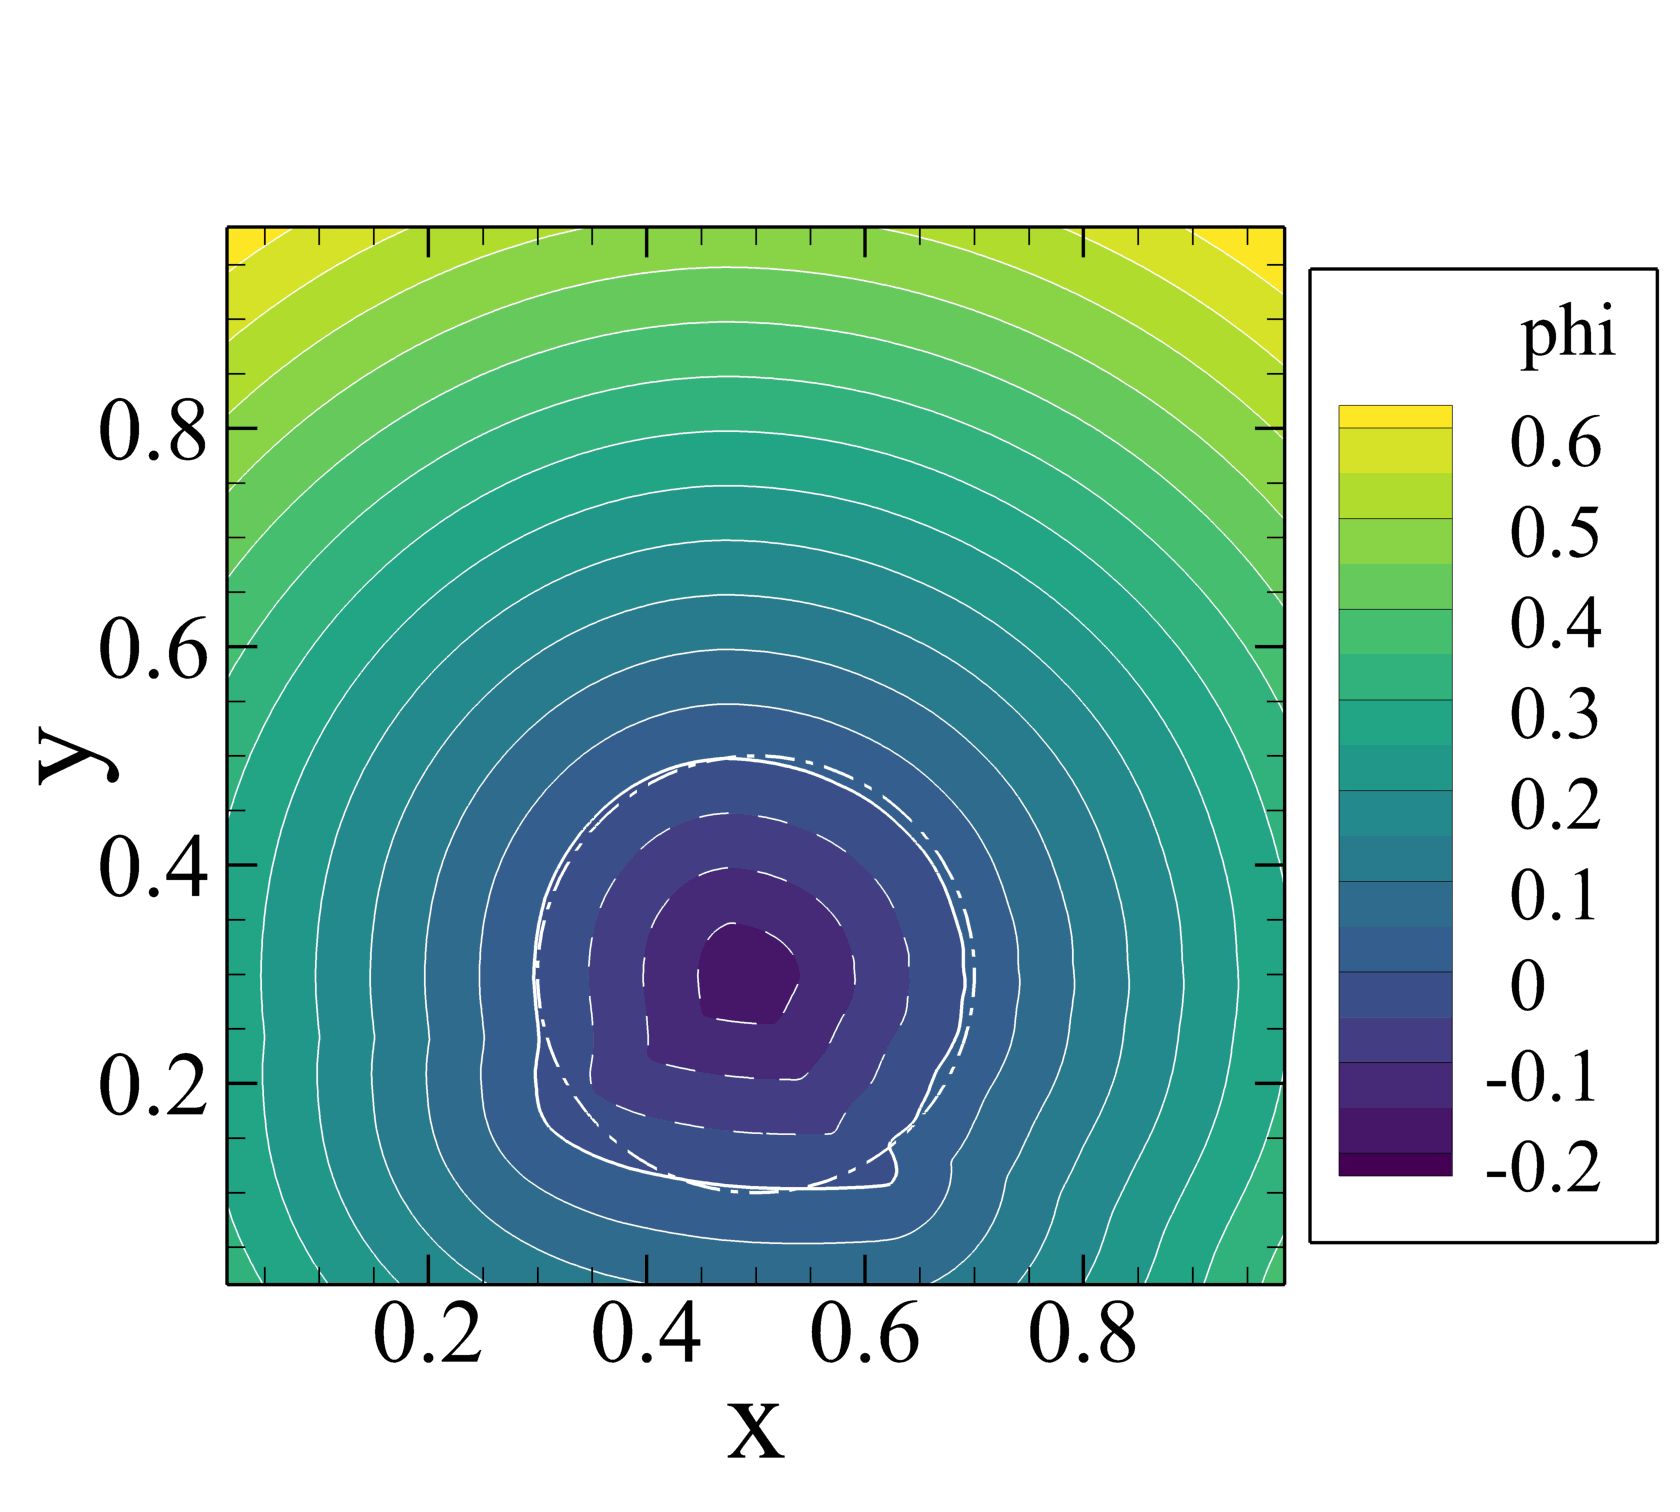
\includegraphics[width=0.24\linewidth]{figure/t2n256r1_2500.png}}
    \subfigure[$N=32$, subcell fix]{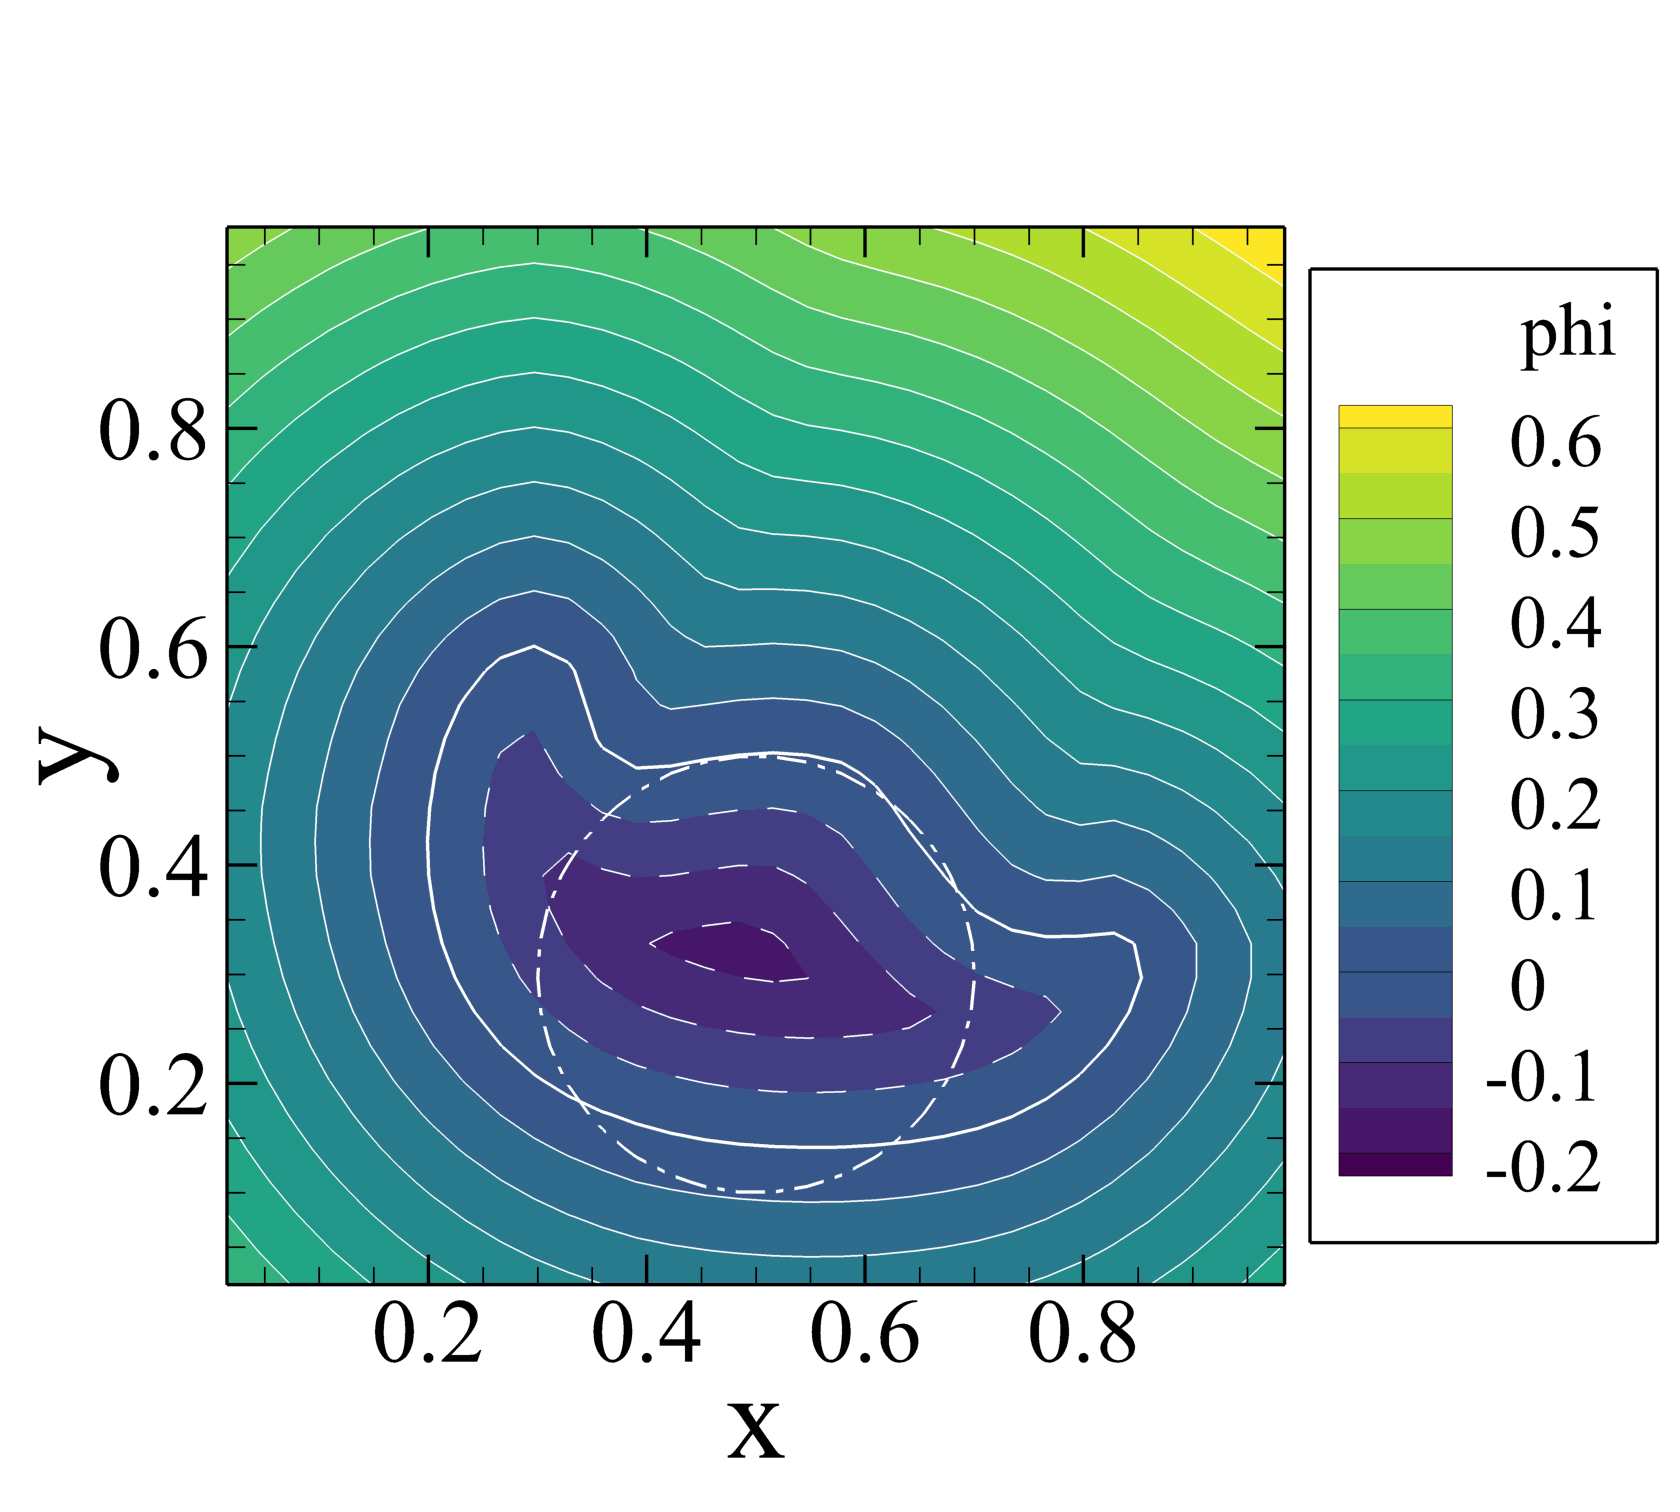
\includegraphics[width=0.24\linewidth]{figure/t2n32r2_2500.png}}
    \subfigure[$N=64$, subcell fix]{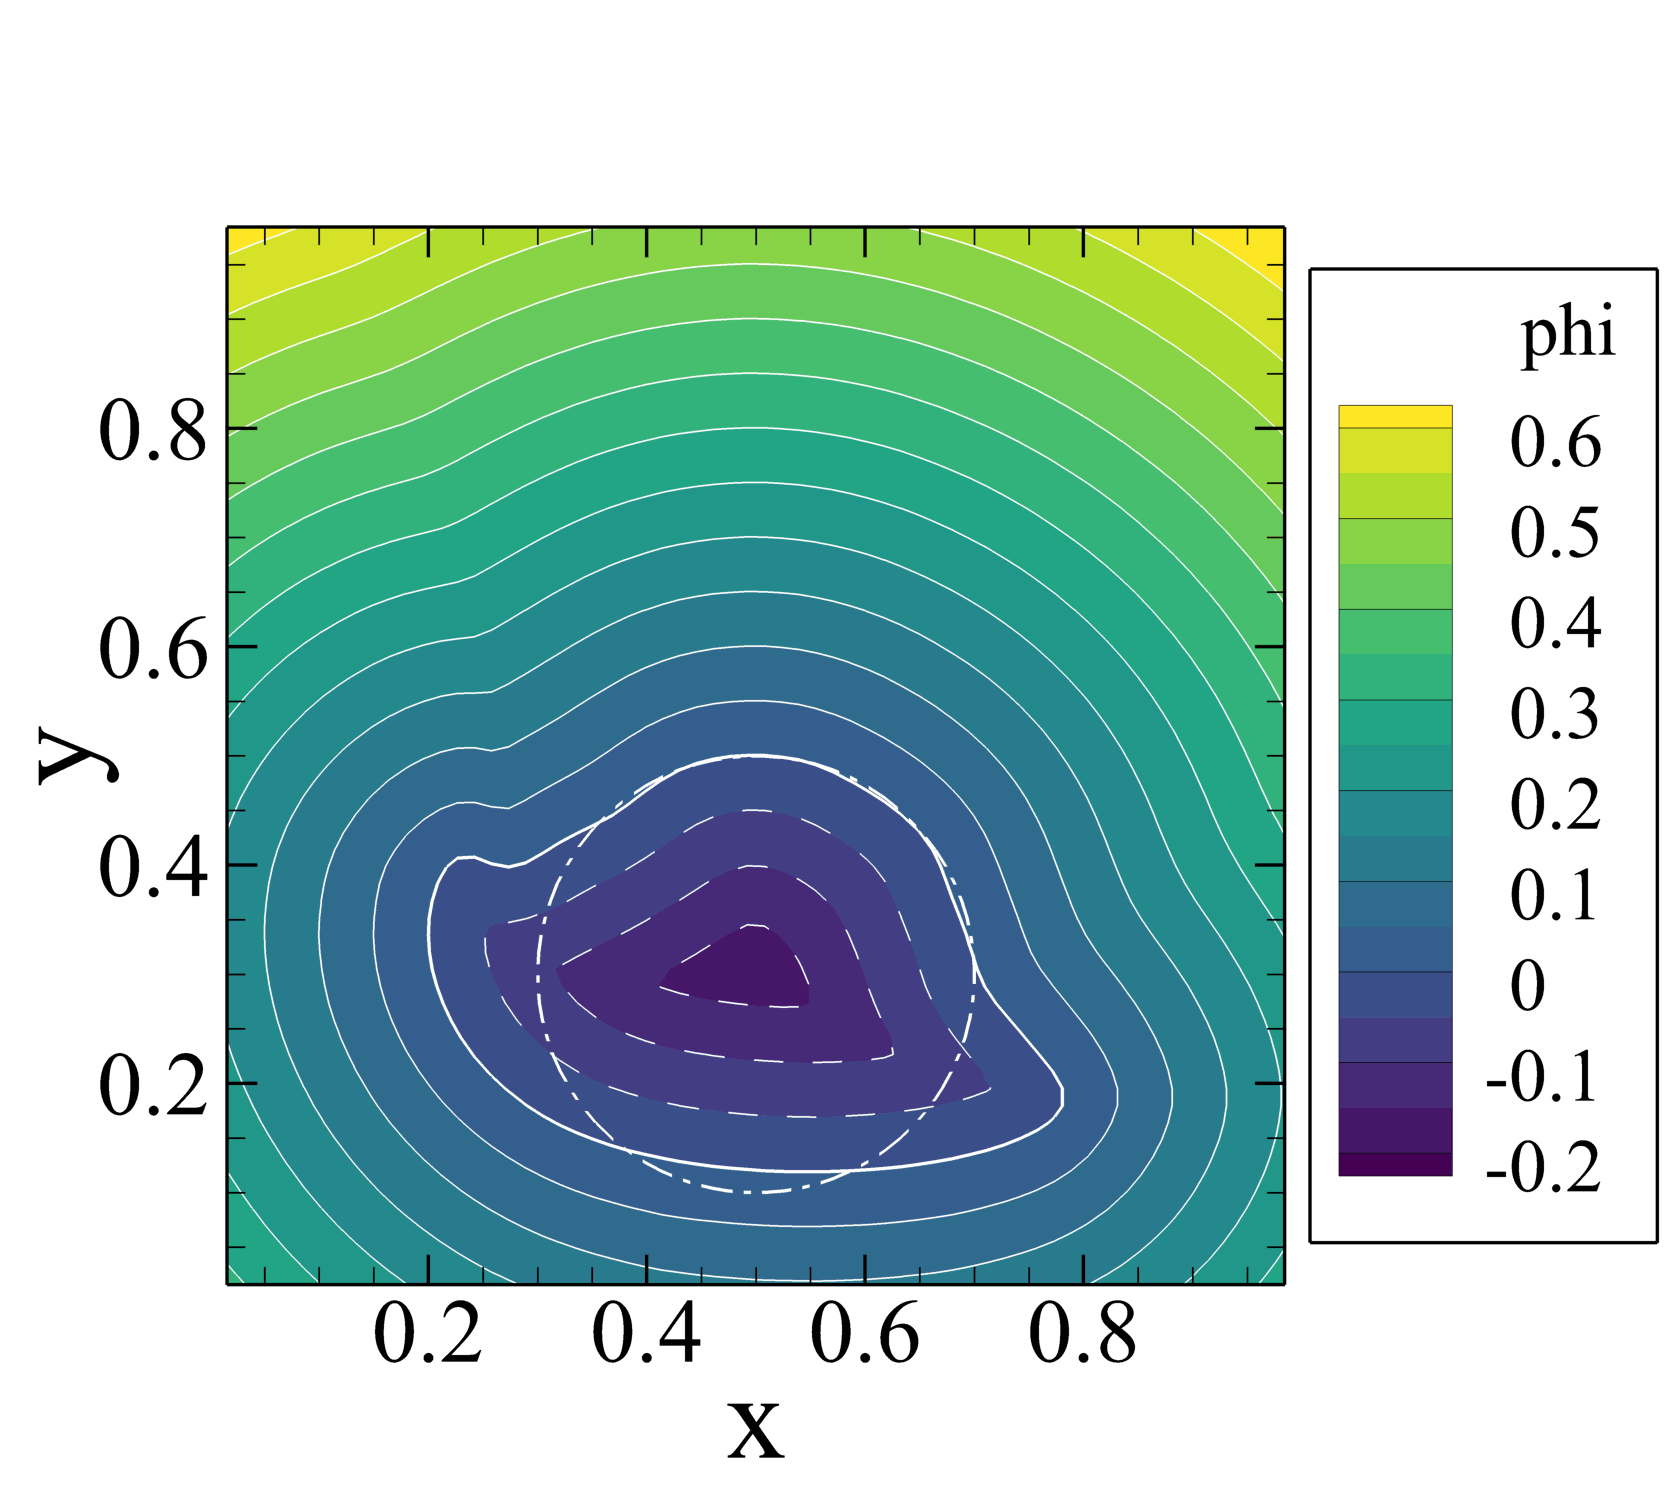
\includegraphics[width=0.24\linewidth]{figure/t2n64r2_2500.png}}
    \subfigure[$N=128$, subcell fix]{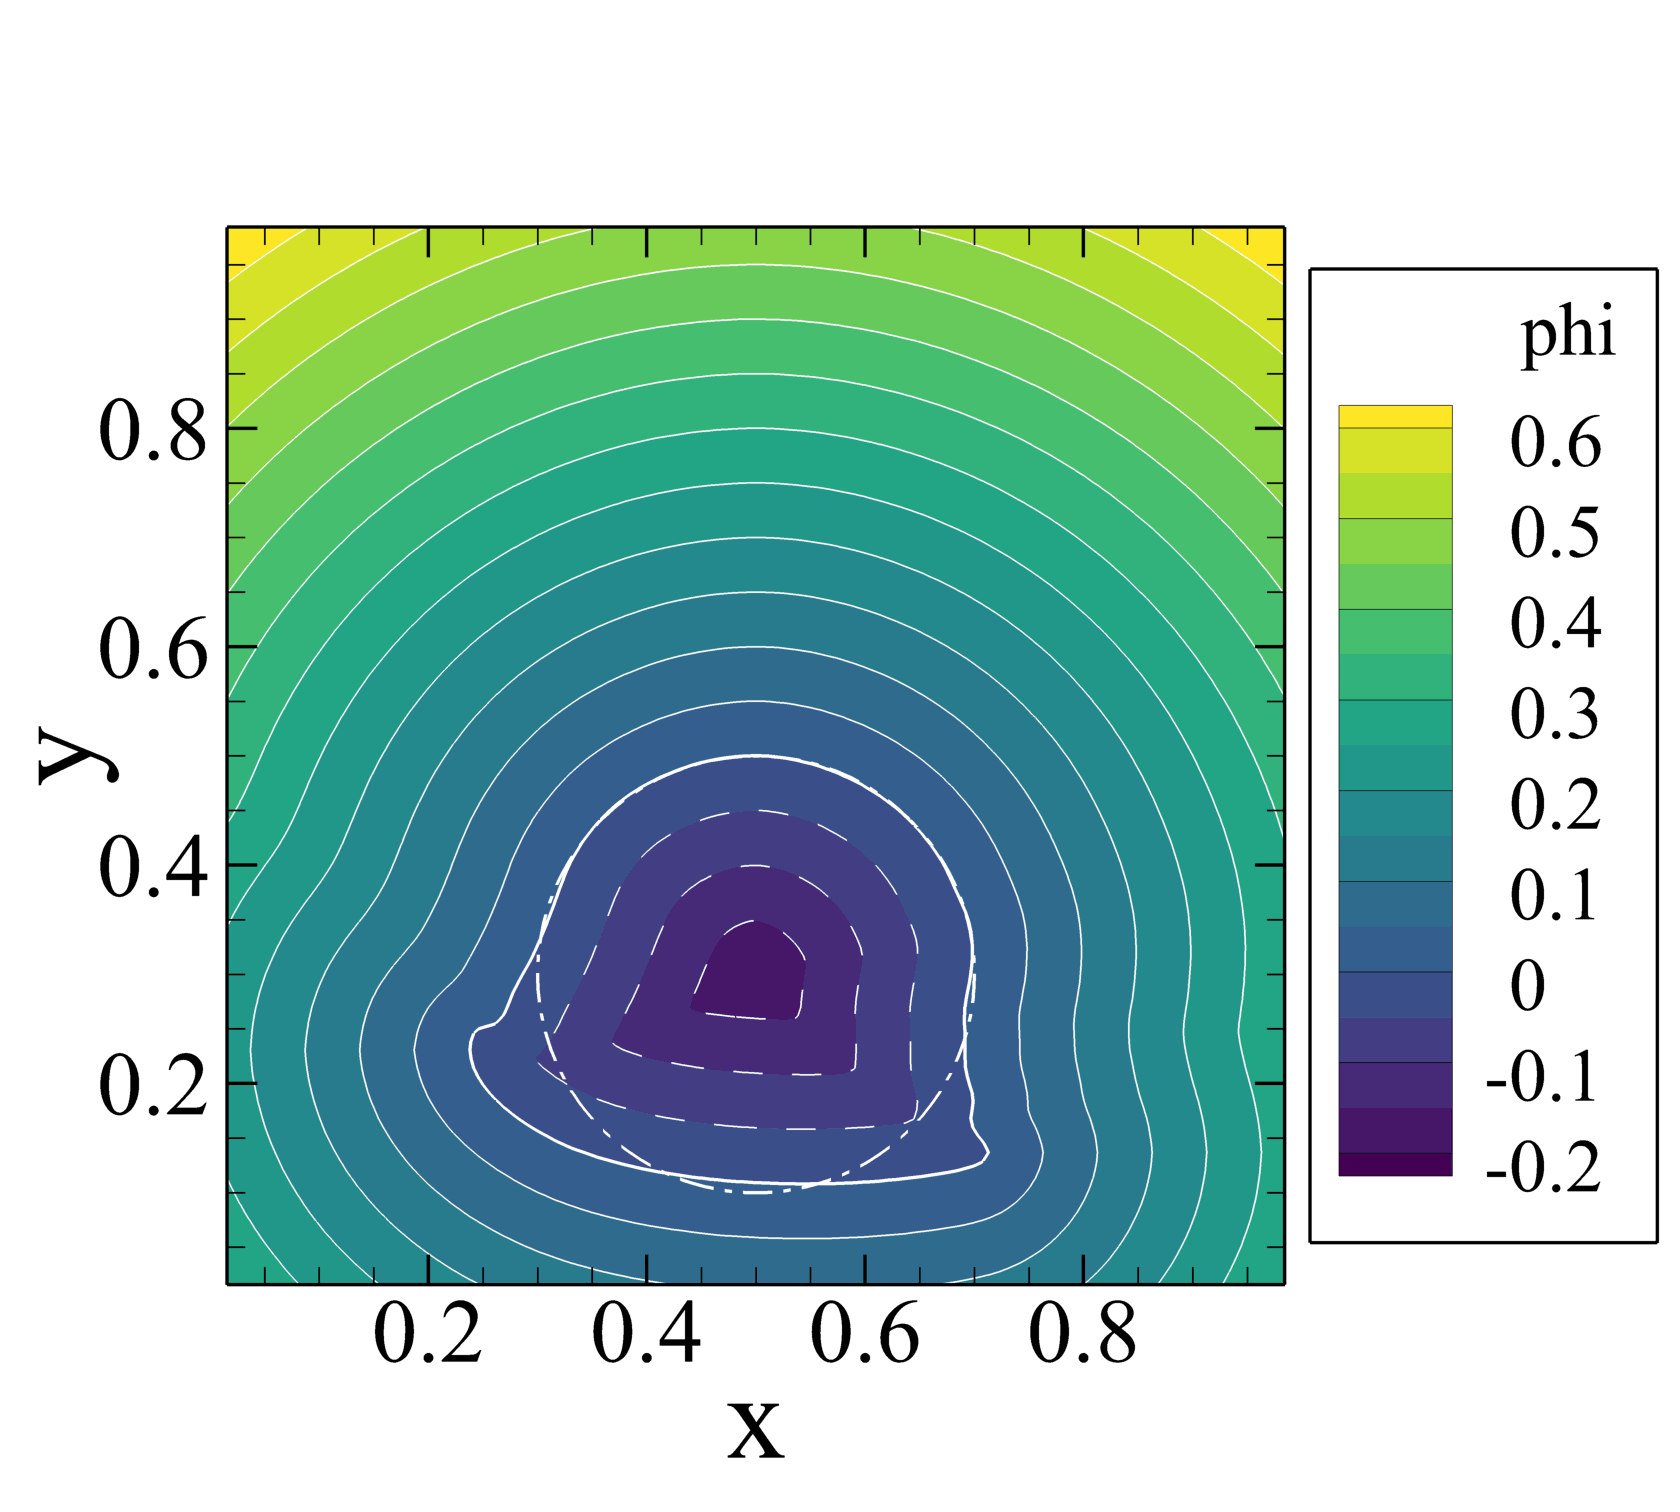
\includegraphics[width=0.24\linewidth]{figure/t2n128r2_2500.png}}
    \subfigure[$N=256$, subcell fix]{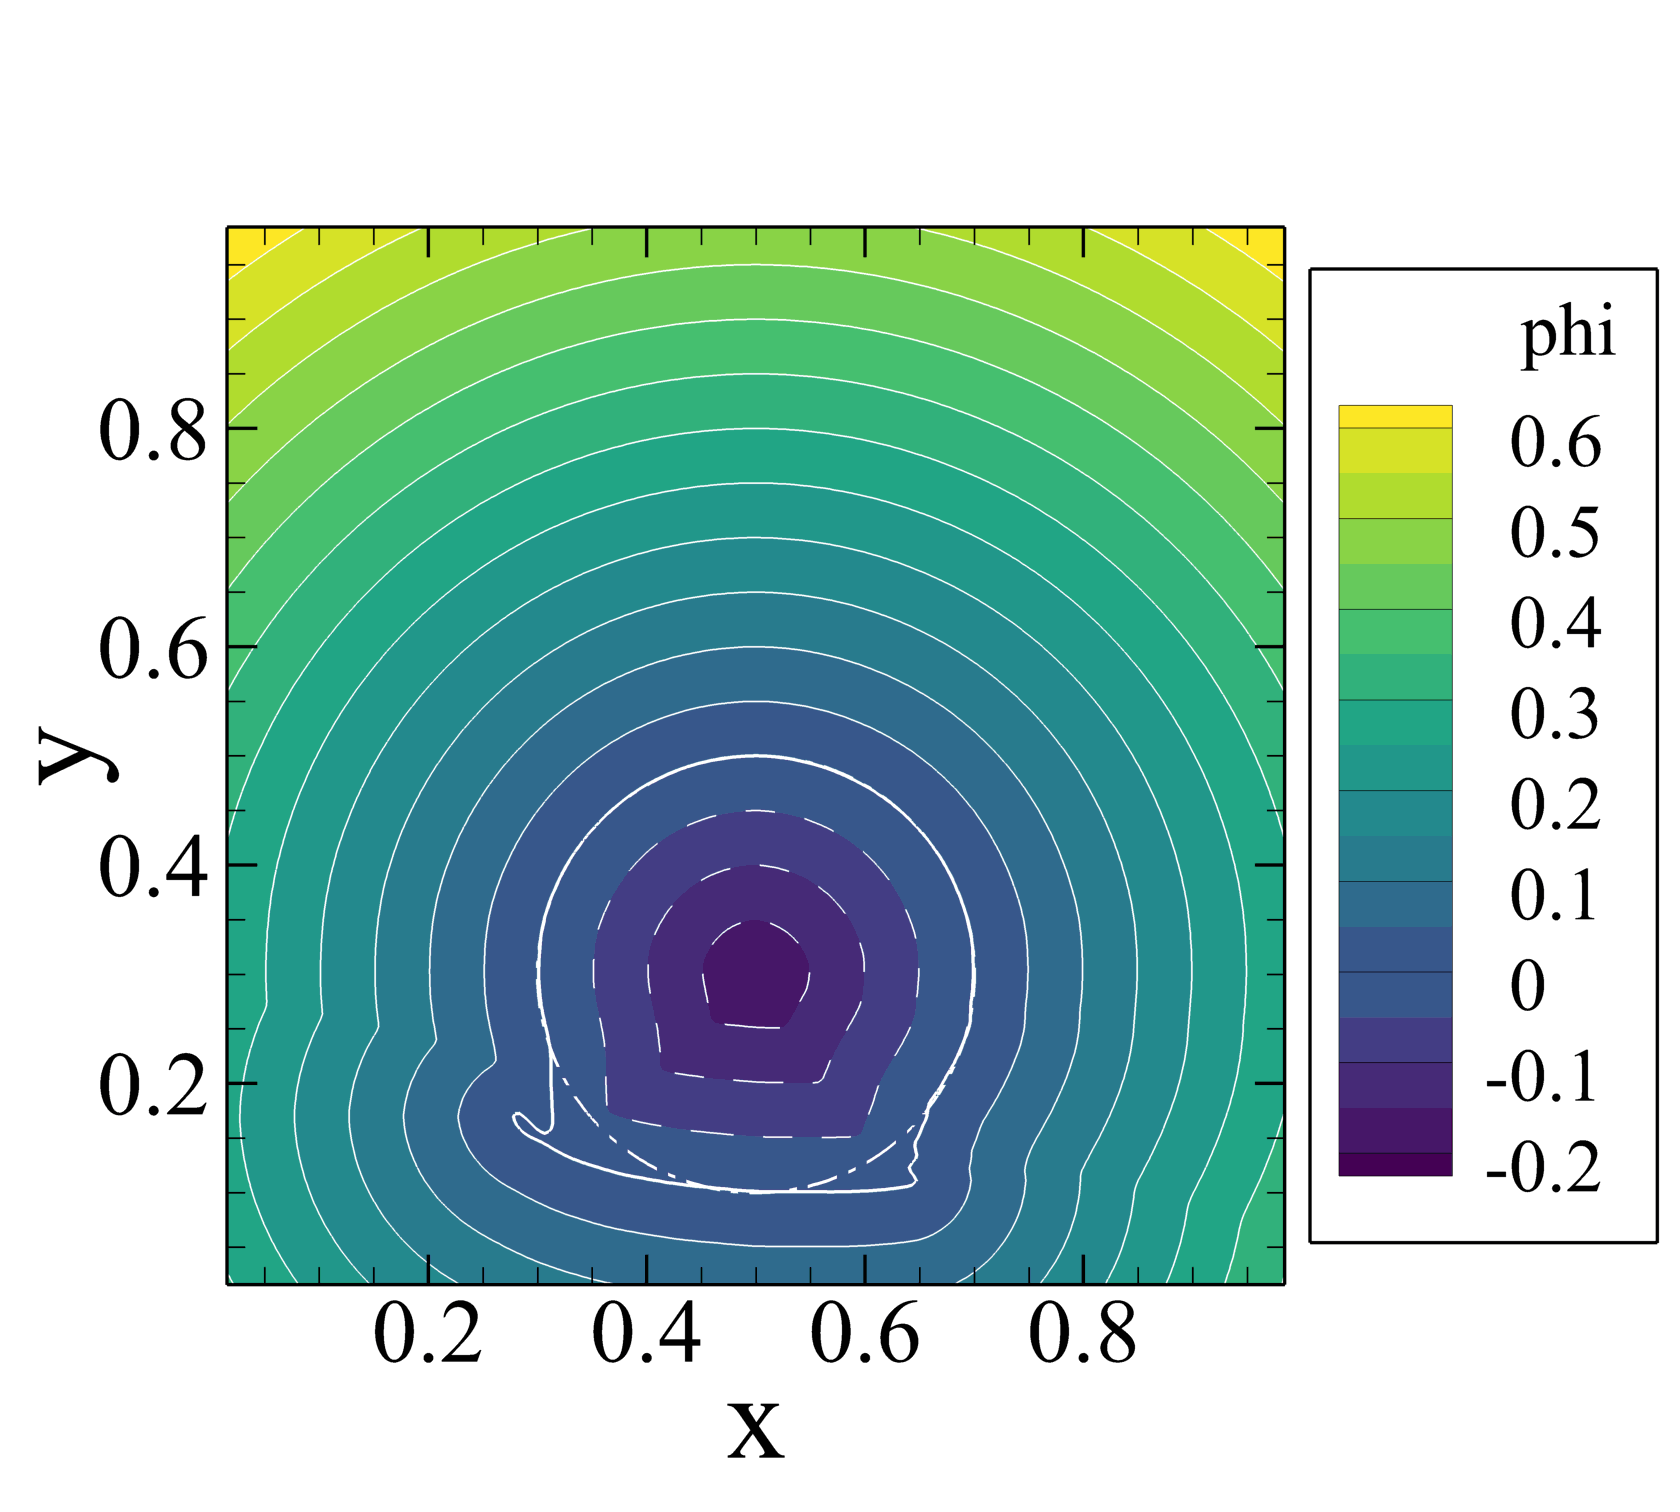
\includegraphics[width=0.24\linewidth]{figure/t2n256r2_2500.png}}
    \caption{\label{fig:return}反演特性校验,不同网格下标准Level Set方法与两种重新初始化方法的比较}
\end{figure}

\subsubsection{变形}
考察液滴在剪切流驱动下持续变形的情况(流场不反转),以$512^2$网格下无重新初始化Level Set方法-QUICK格式结果作为基准。对比了$512^2$网格加入Subcell fix重新初始化,$128^2$网格无重新初始化、简单重新初始化、Subcell fix重新初始化等方法下,推进至$t=1,\ 2,\ 3$时刻的液滴形态,结果见\autoref{fig:deform512}、\autoref{fig:deform128}。

\begin{figure}[h]
    \centering
    \subfigure[$t=1$]{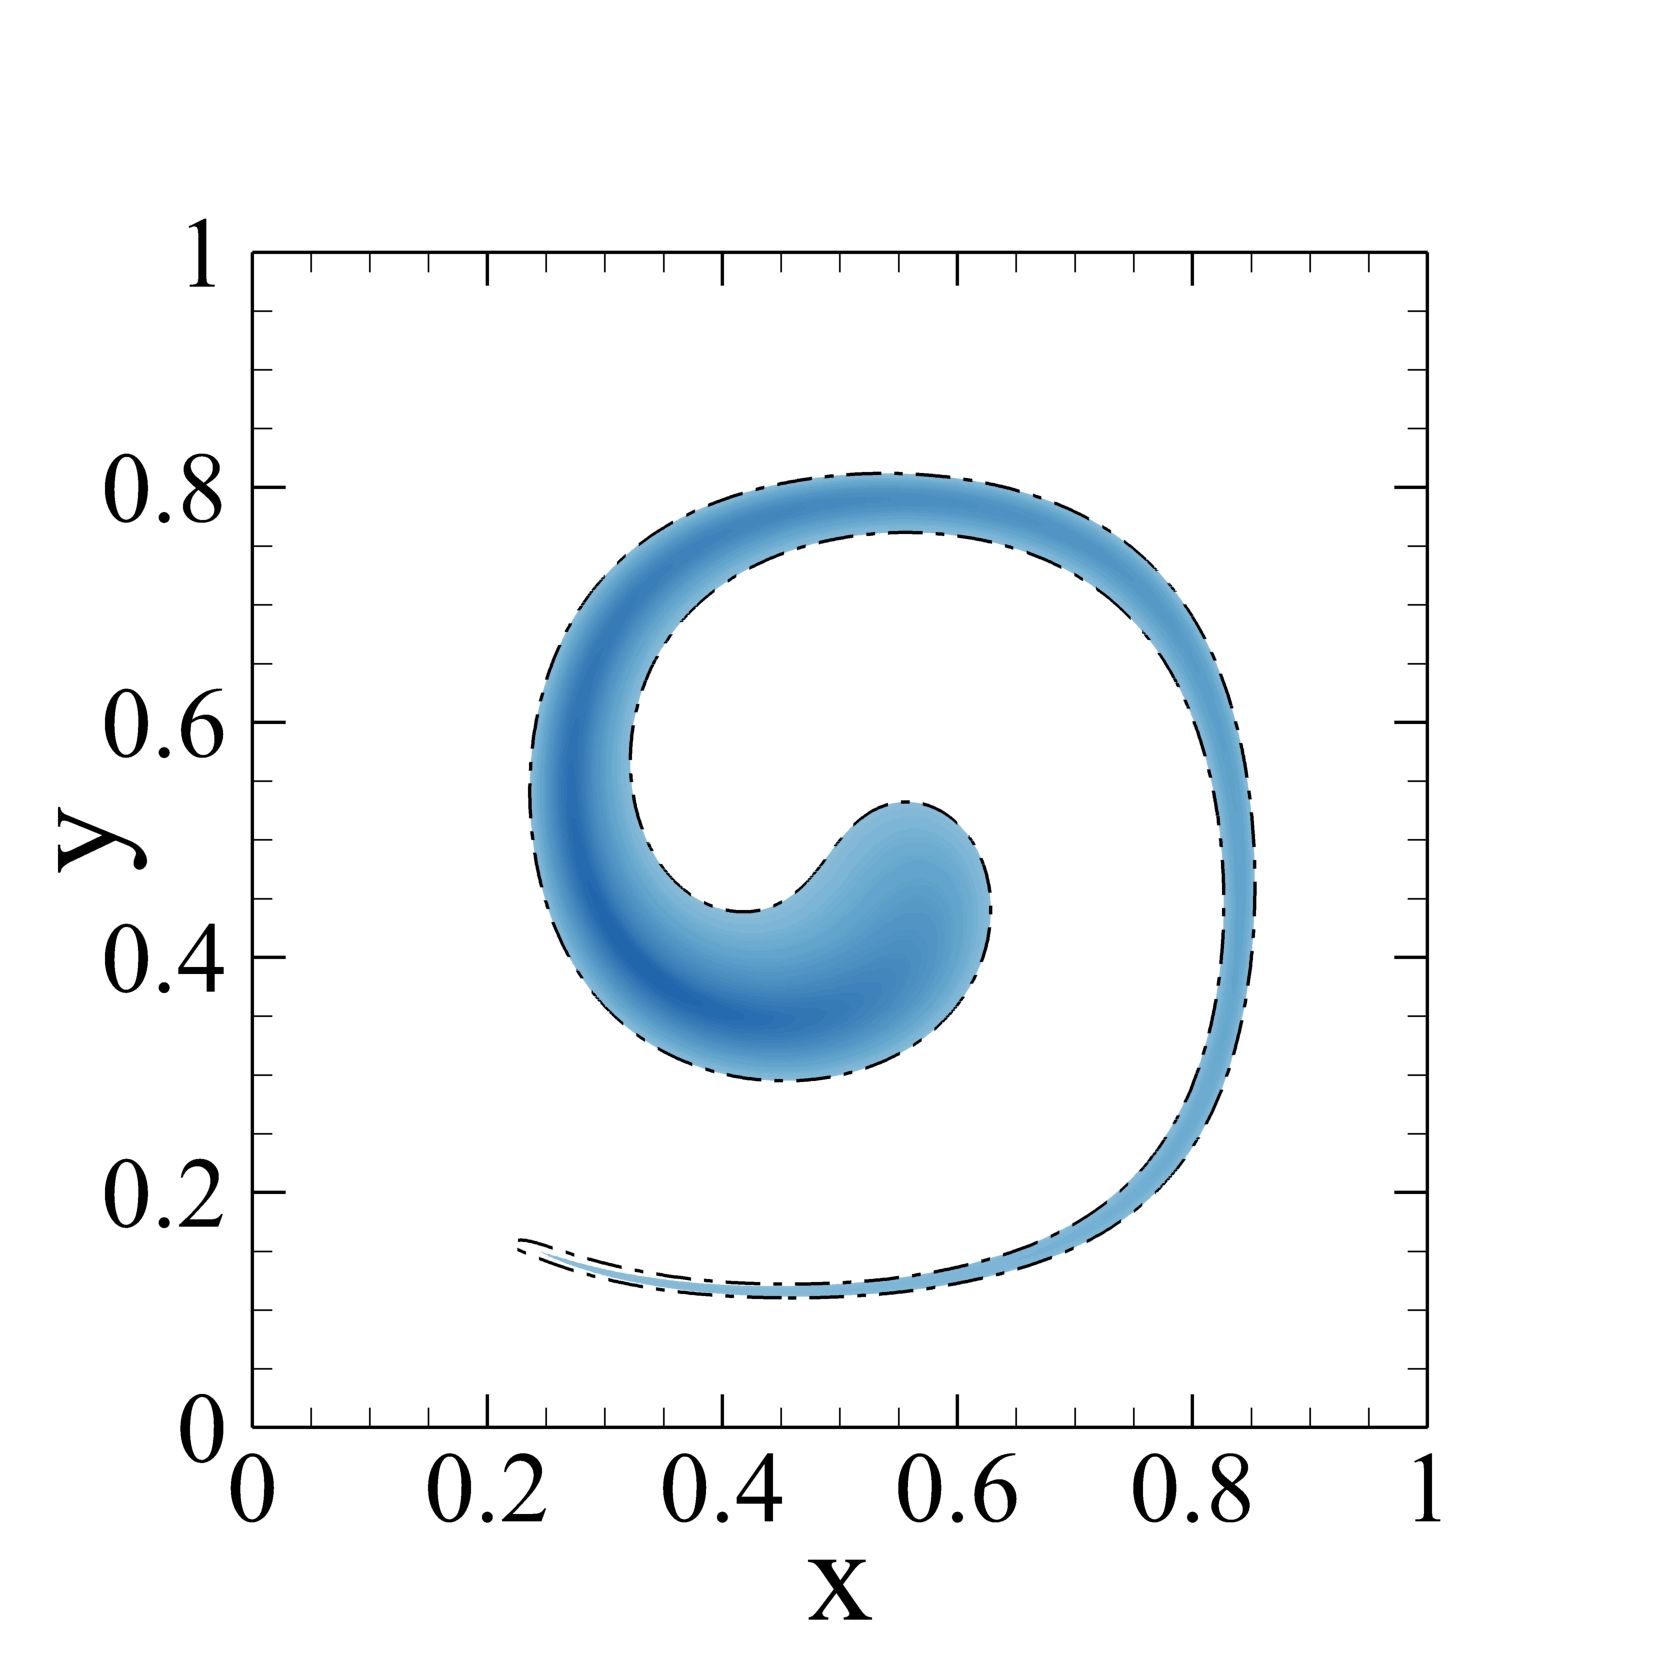
\includegraphics[width=0.3\linewidth]{figure/deform_512_t10.png}}
    \subfigure[$t=2$]{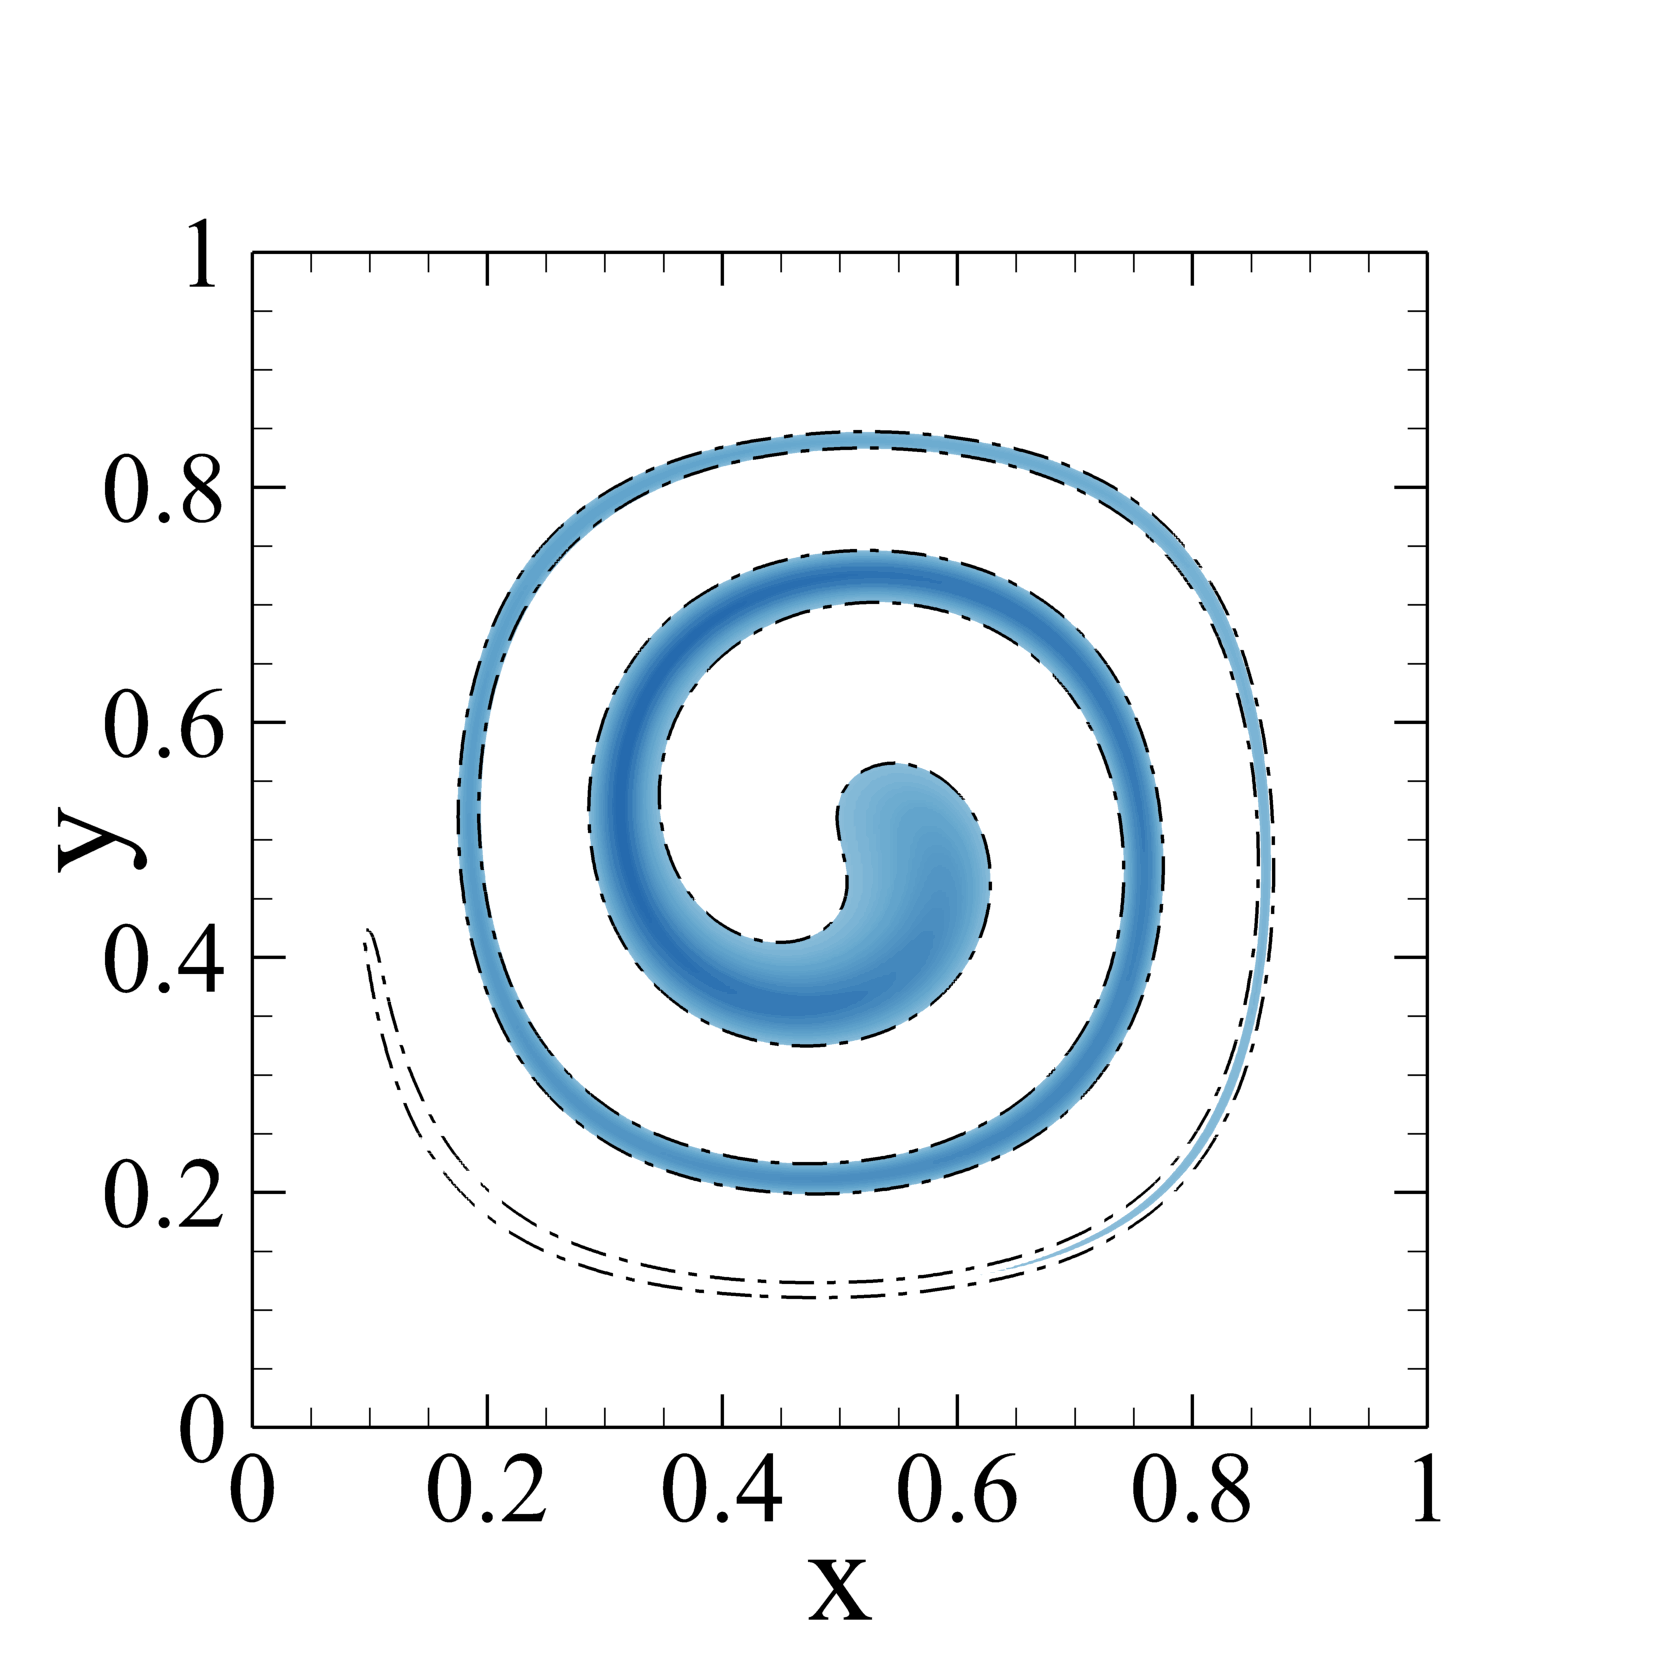
\includegraphics[width=0.3\linewidth]{figure/deform_512_t20.png}}
    \subfigure[$t=3$]{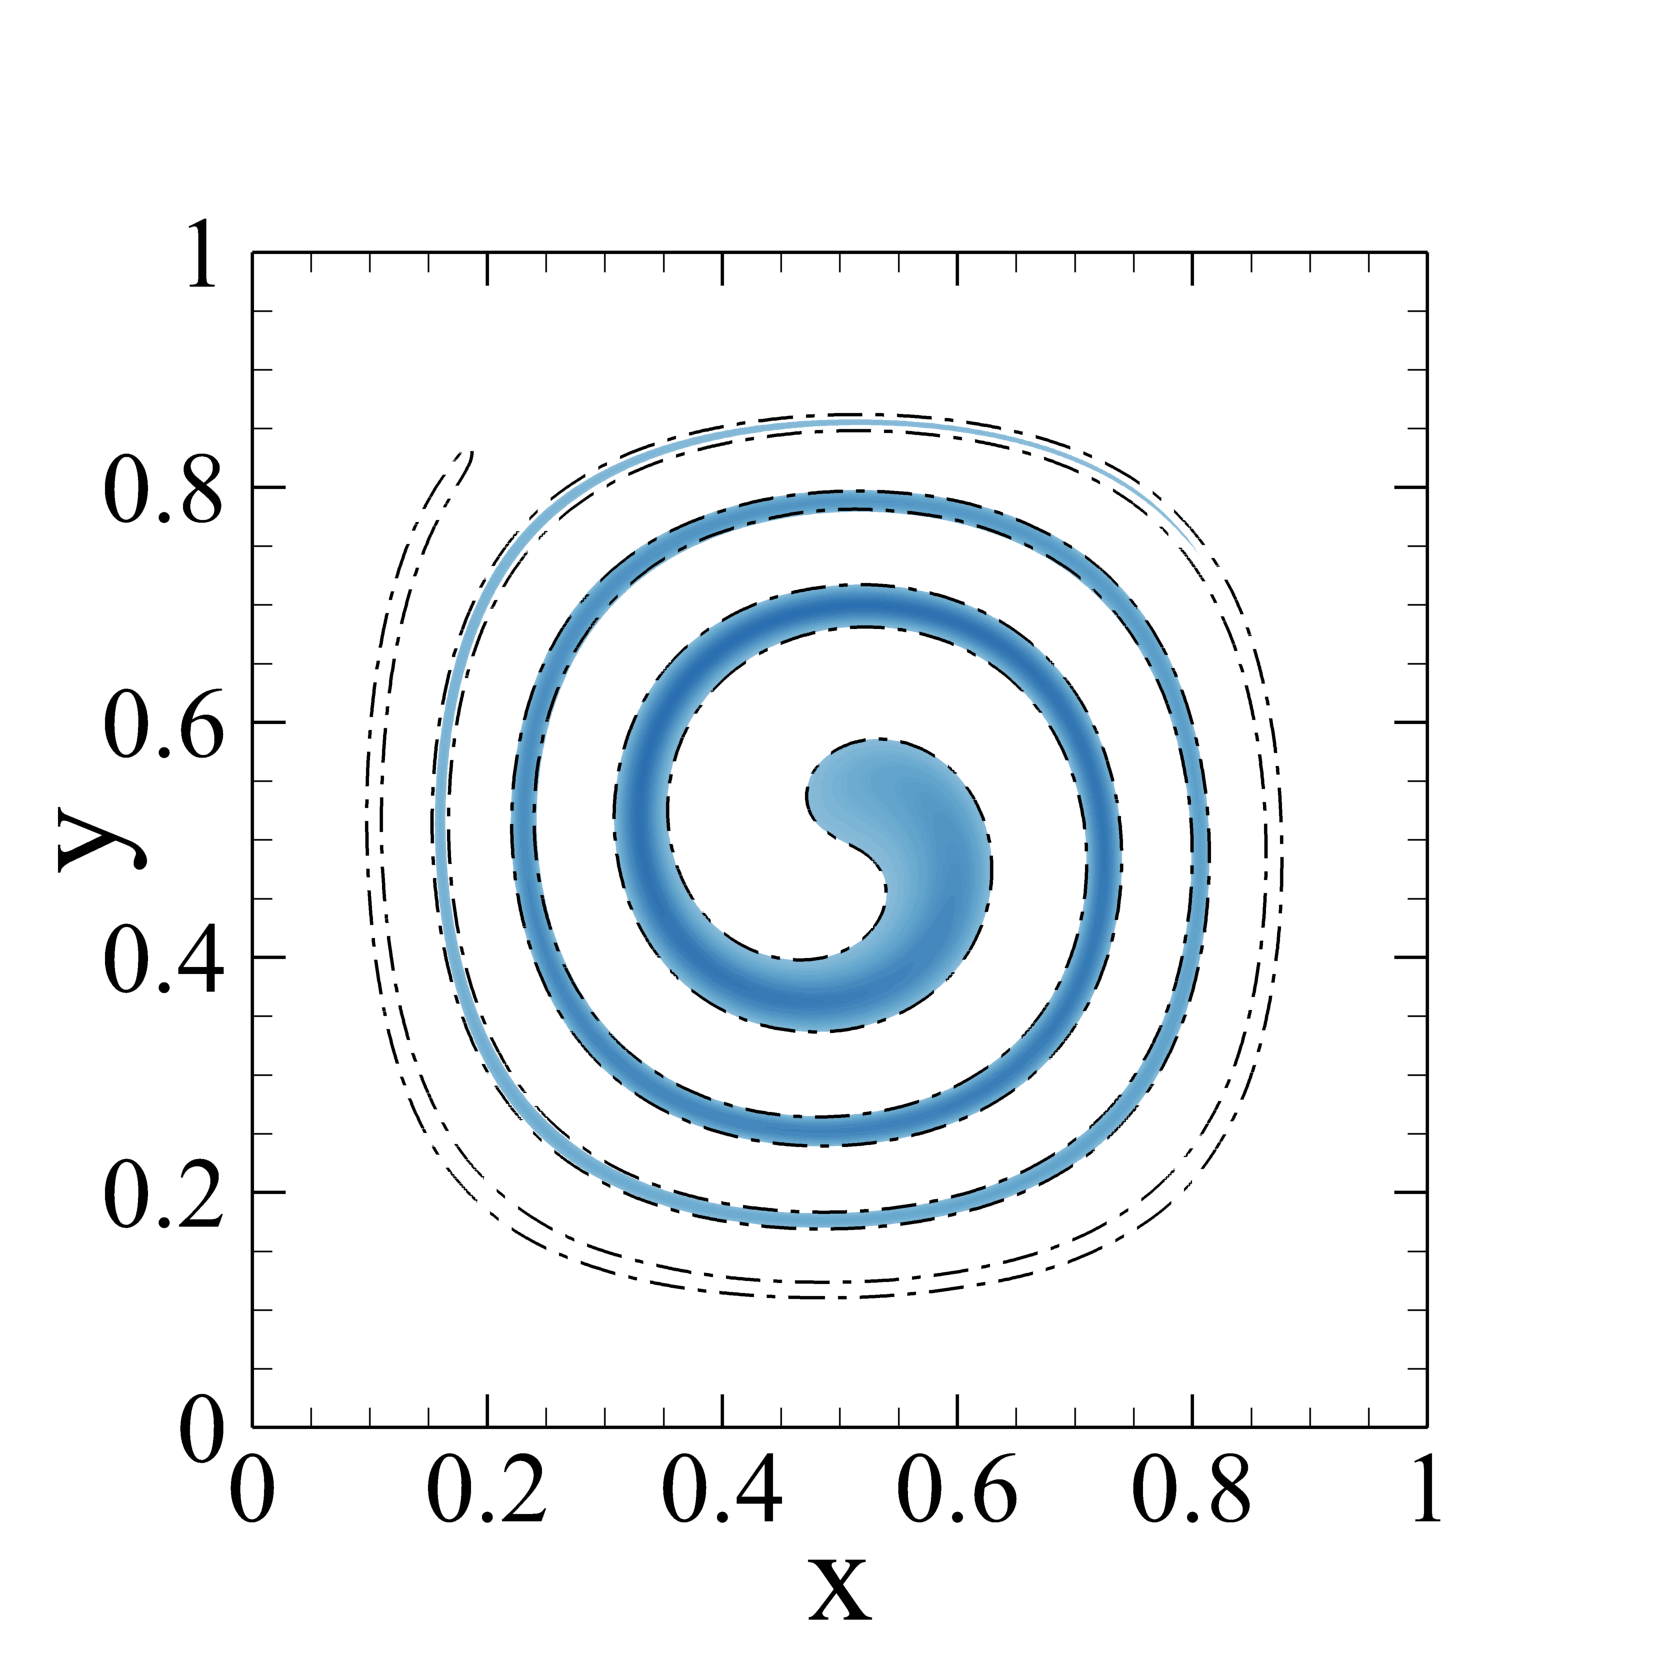
\includegraphics[width=0.3\linewidth]{figure/deform_512_t30.png}}
    \caption{\label{fig:deform512}$512^2$网格下基础Level Set方法(基准,蓝底)和加入Subcell fix重新初始化后的结果(黑色点划线),可以看到Subcell fix重新初始化引入了额外的体积增加。}
\end{figure}

\begin{figure}[h]
    \centering
    \subfigure[$t=1$]{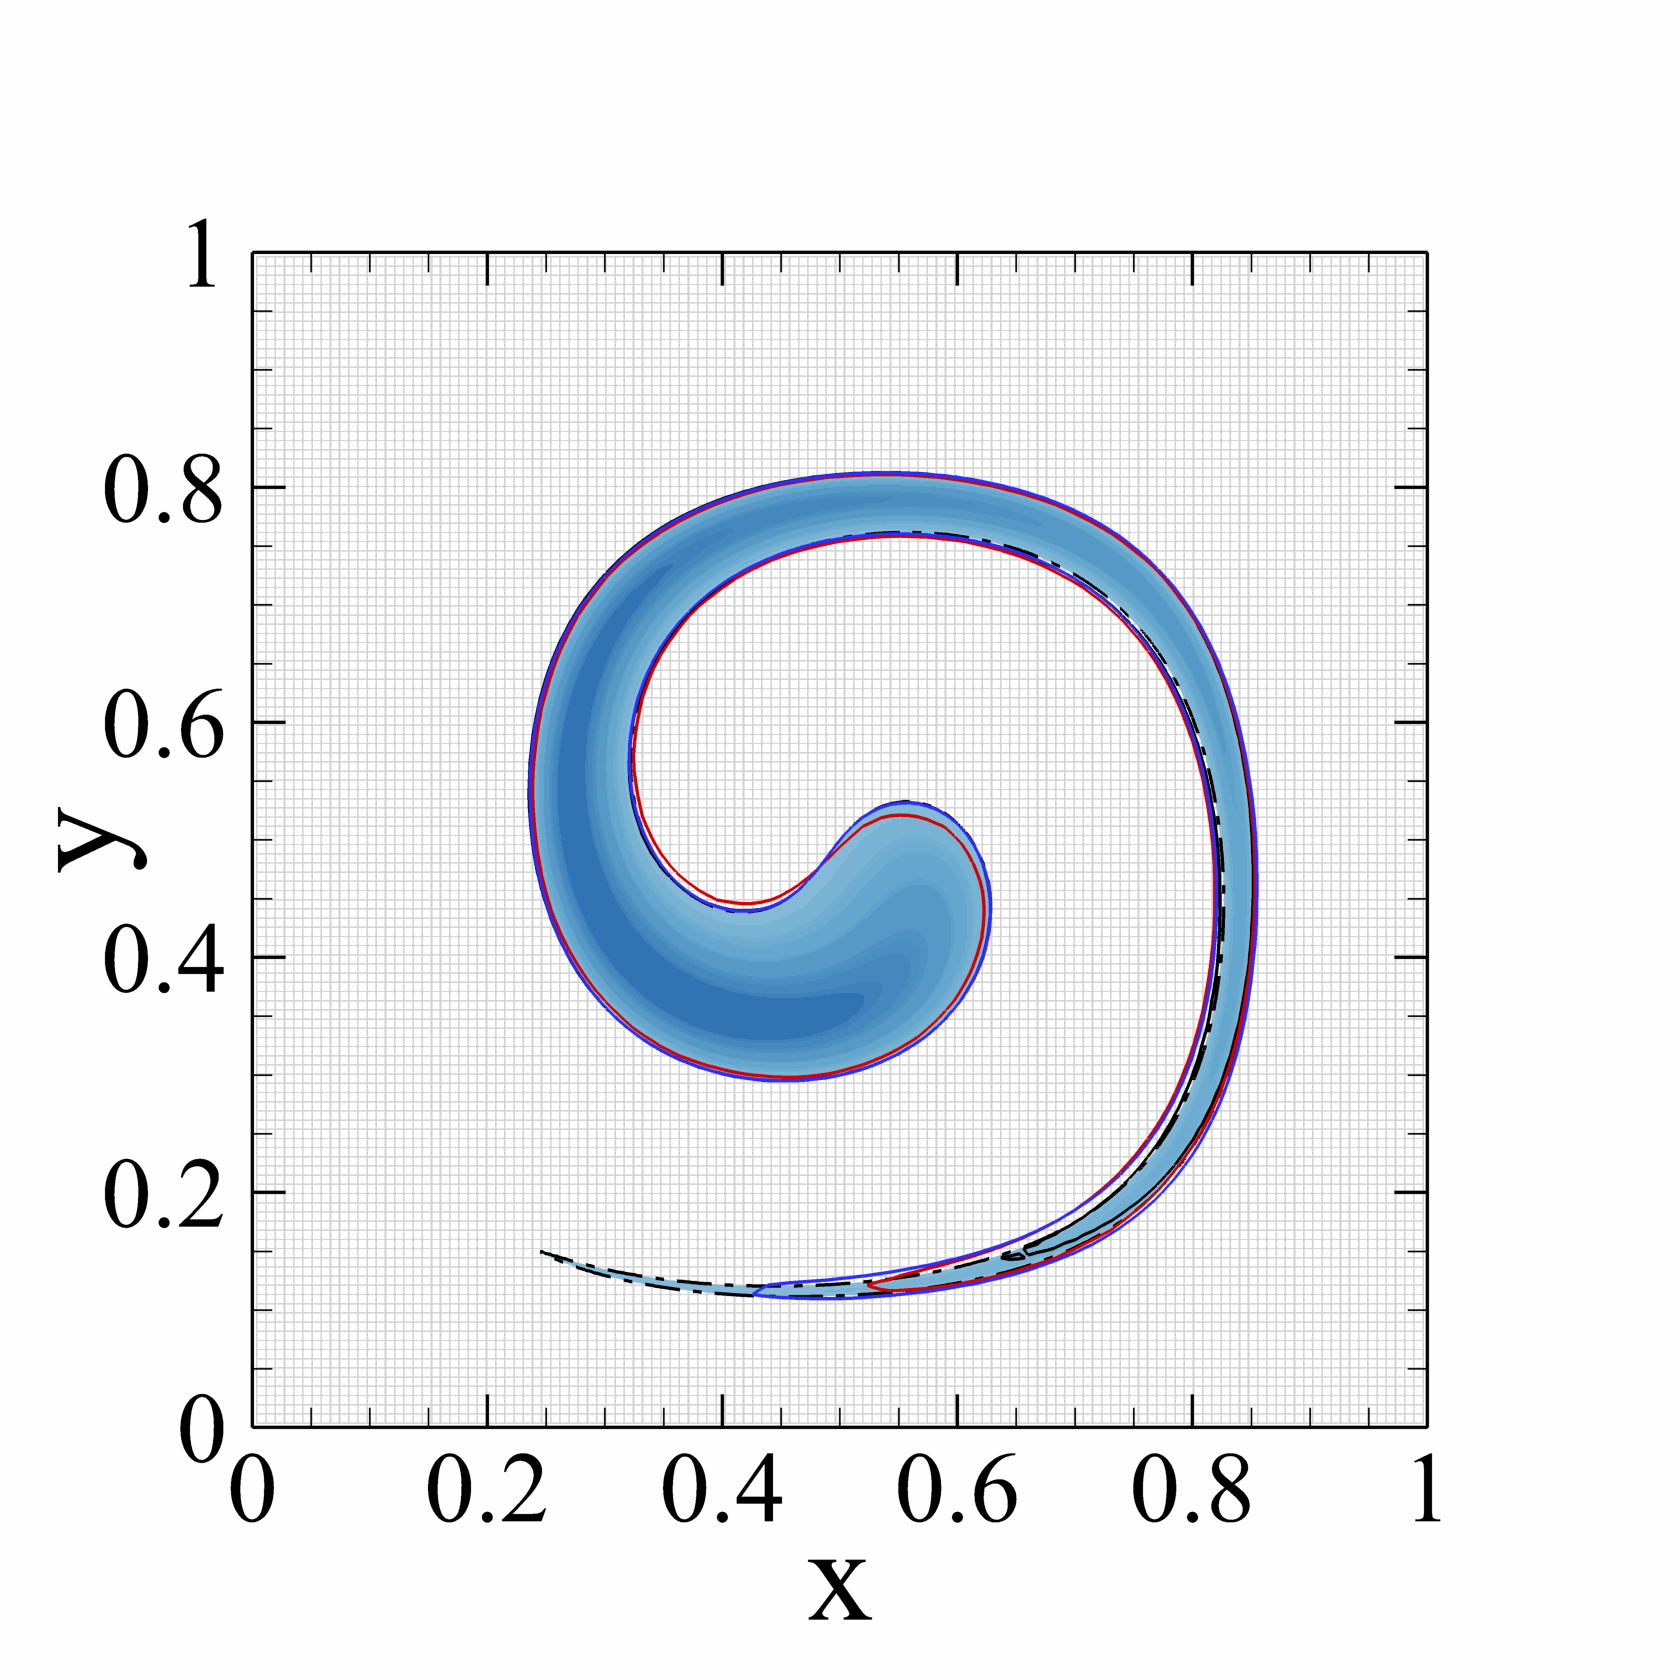
\includegraphics[width=0.3\linewidth]{figure/deform_all_t10.png}}
    \subfigure[$t=2$]{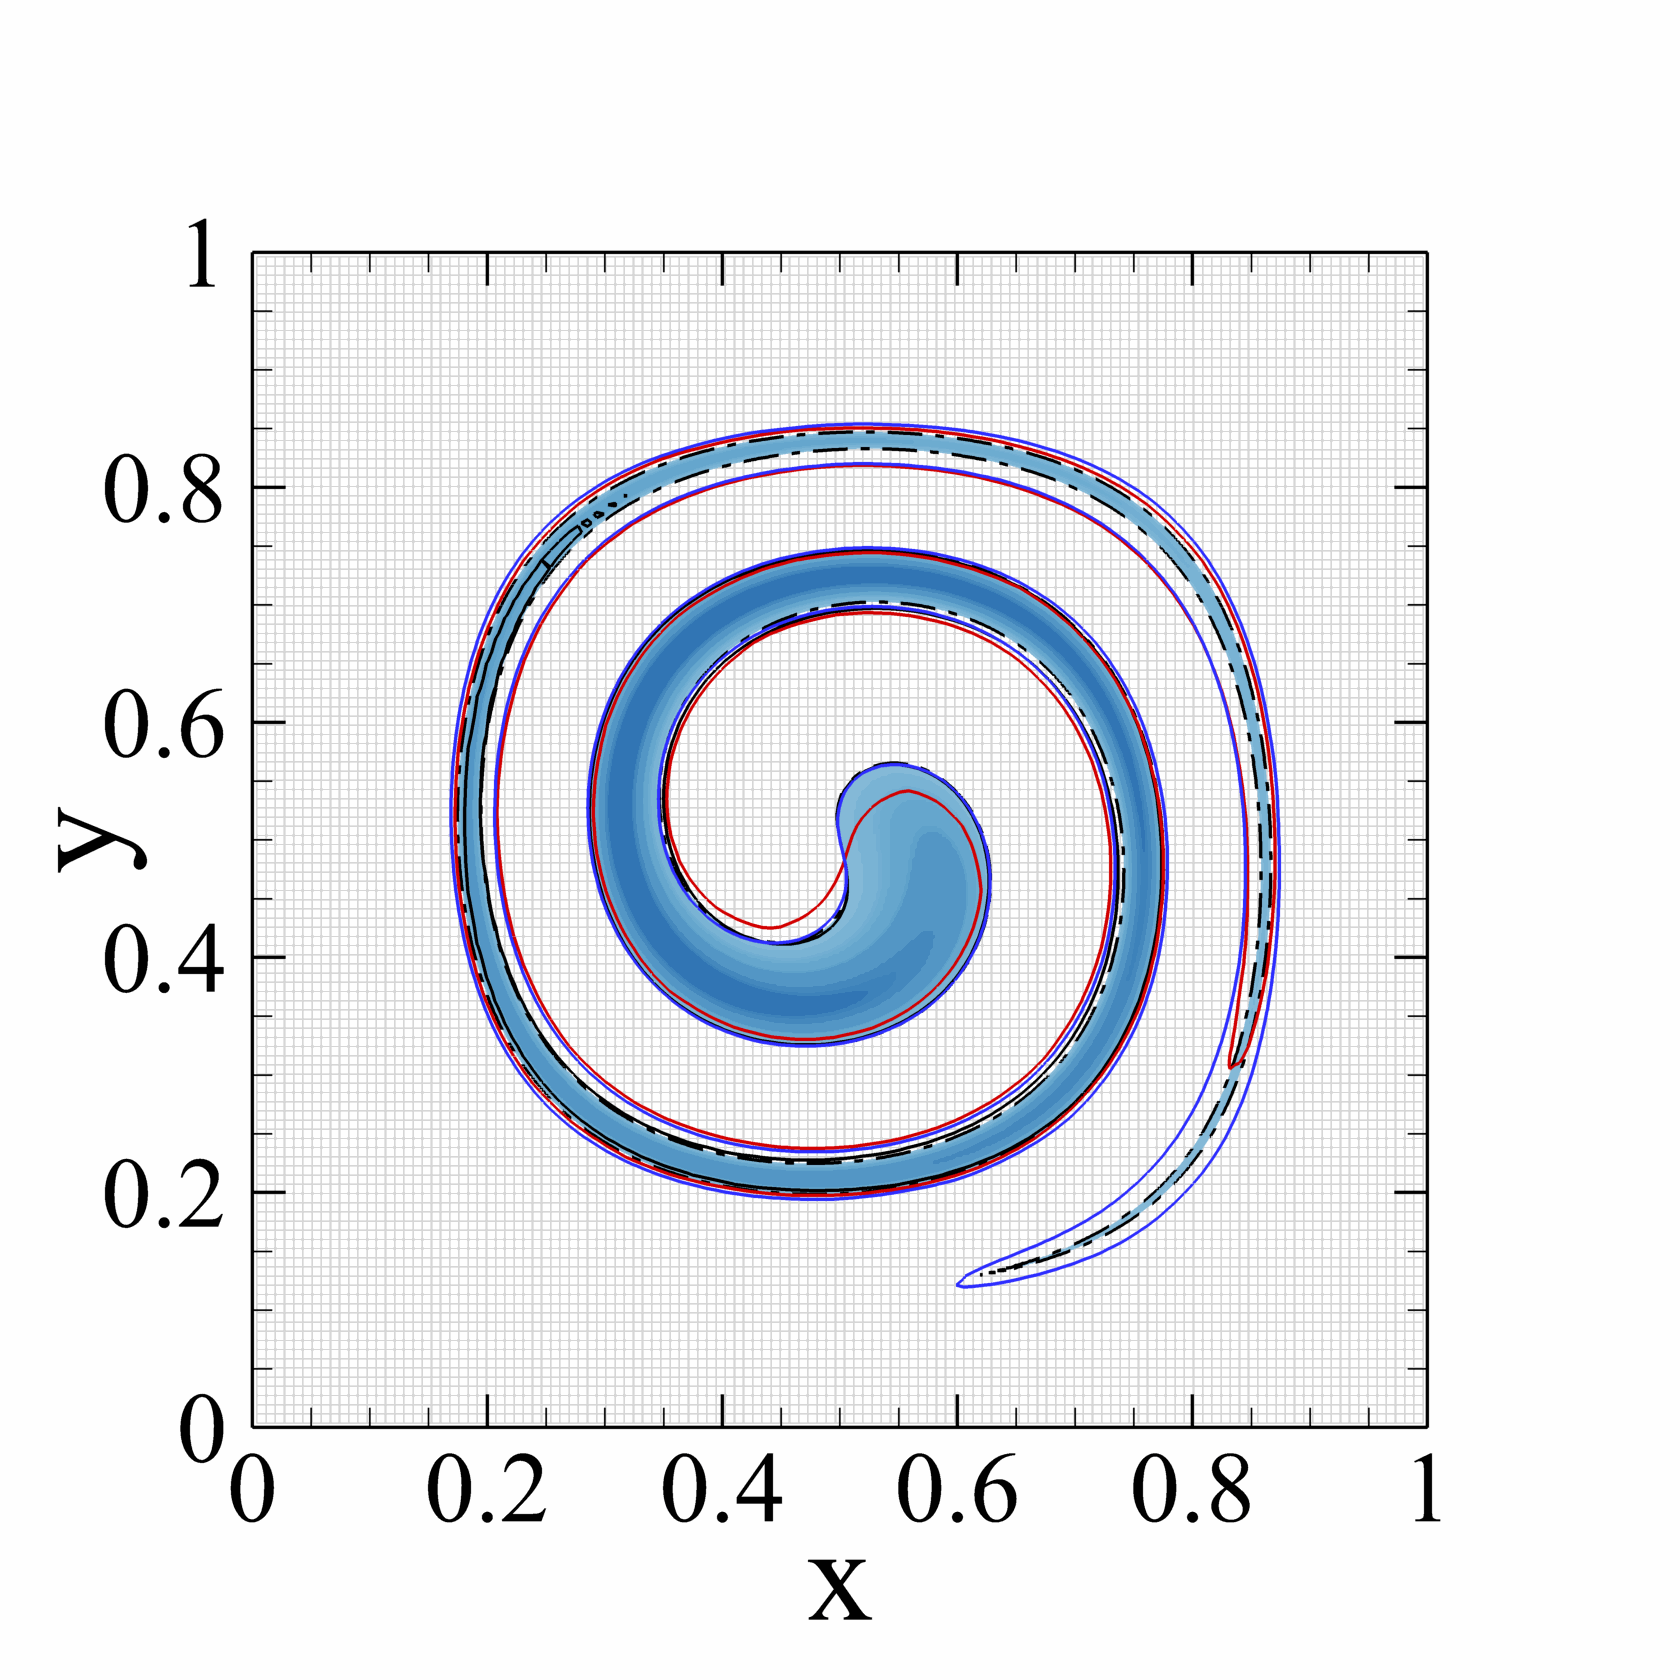
\includegraphics[width=0.3\linewidth]{figure/deform_all_t20.png}}
    \subfigure[$t=3$]{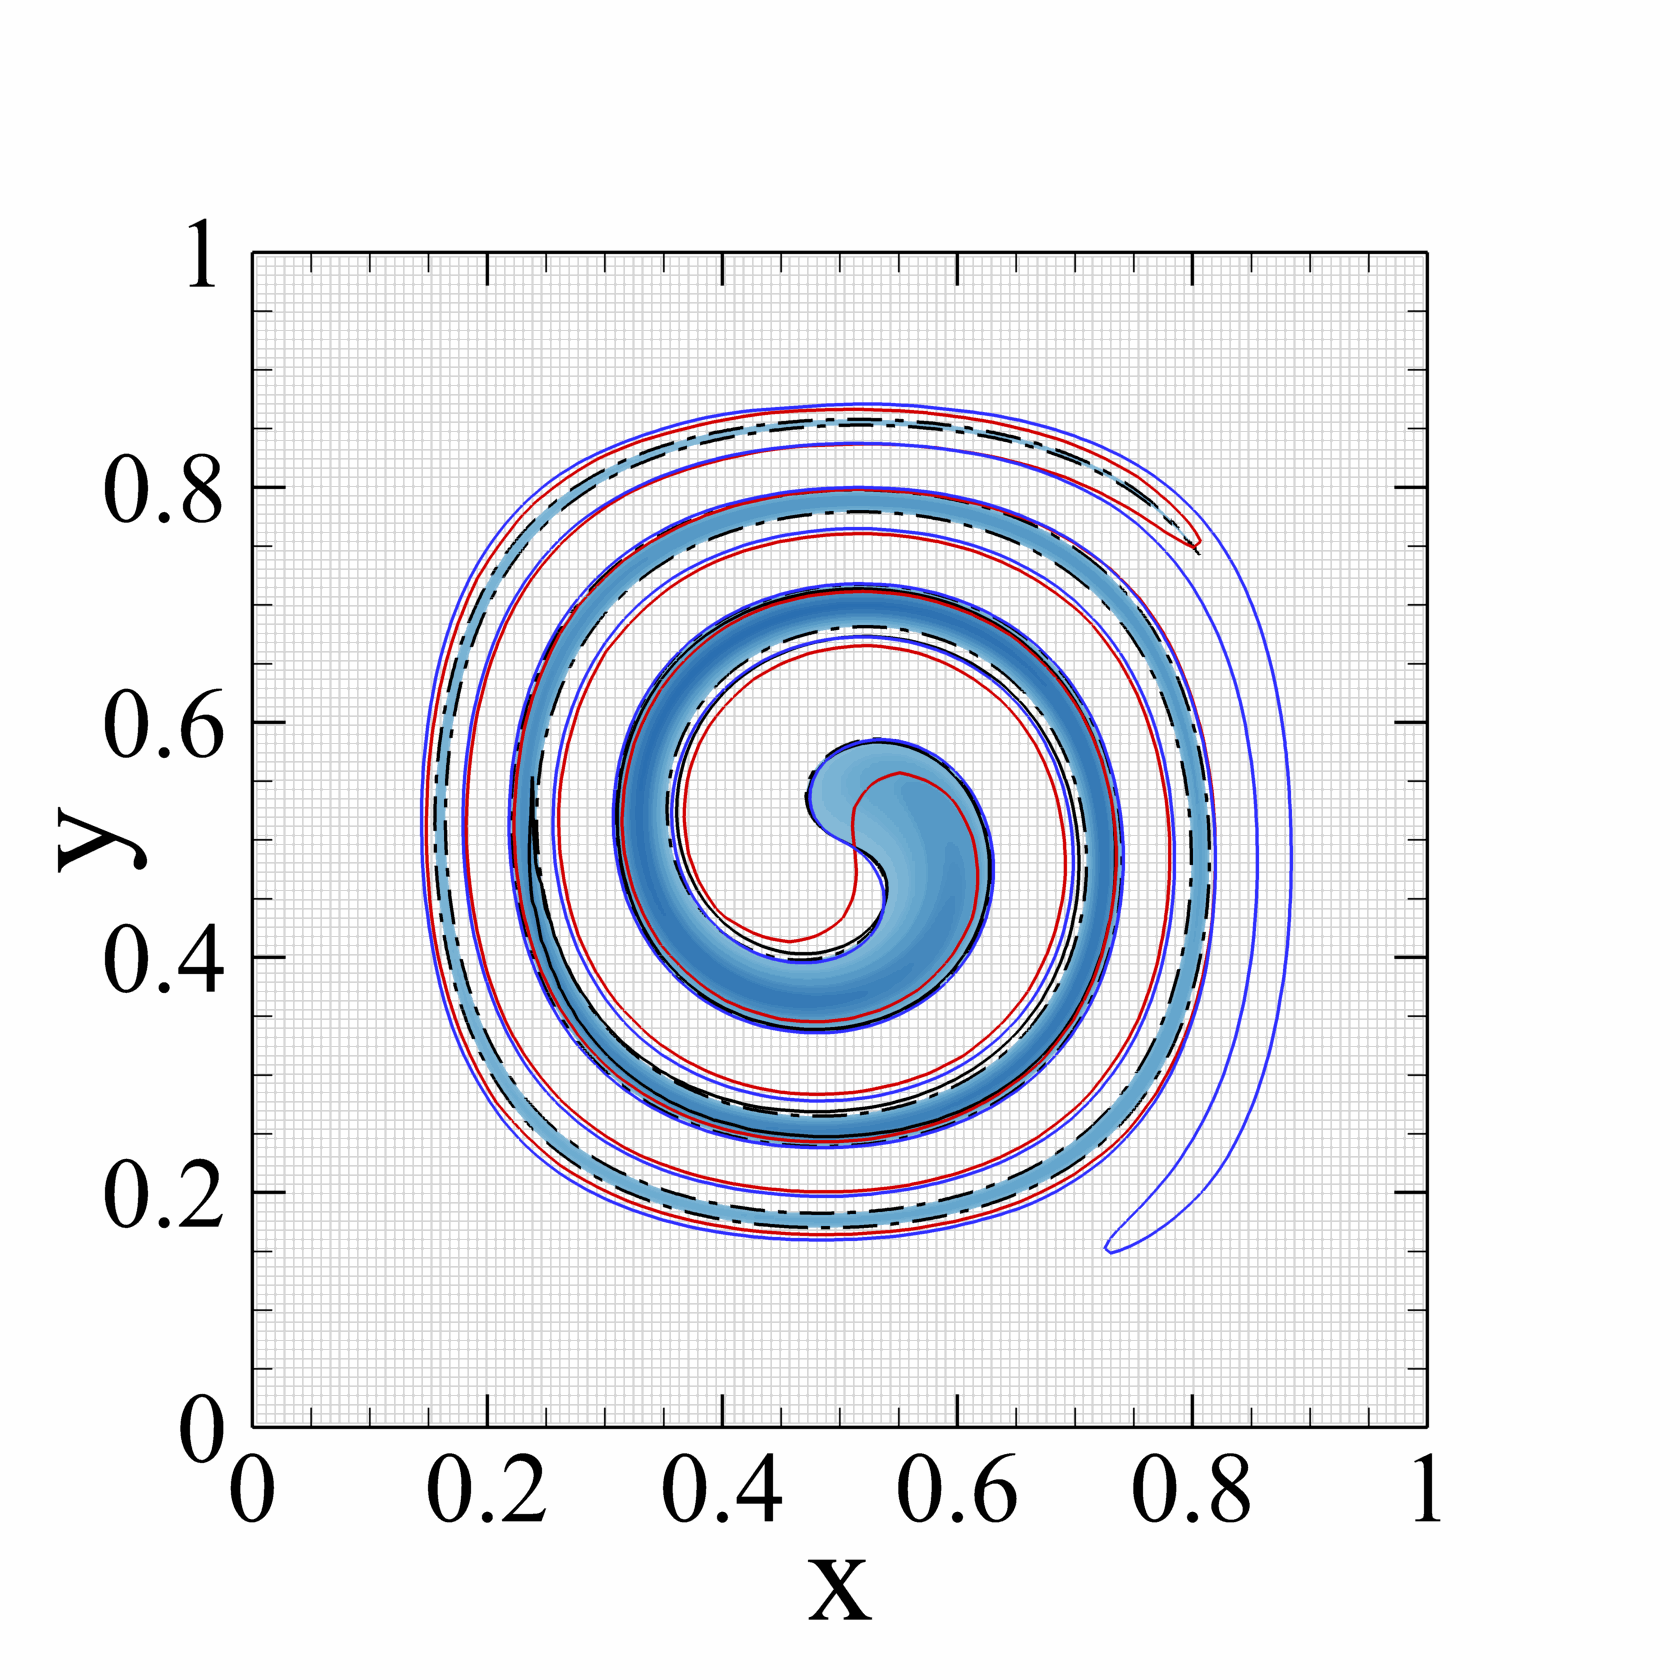
\includegraphics[width=0.3\linewidth]{figure/deform_all_t30.png}}
    \caption{\label{fig:deform128}$128^2$网格下各方法结果(实线):基础Level Set(黑);简单重新初始化(红);Subcell fix重新初始化。}
\end{figure}

可以发现,随着时间推进,当网格不足以分辨变形液滴的细长尾部时,基础Level Set方法会出现显著的质量/体积损失。与之相反的,加入Subcell fix重新初始化步骤的结果会在尾部出现非物理的质量/体积增加,导致尾部更宽更长。正是由于网格、重新初始化方法不足以精确捕捉细长尾部,使得\autoref{fig:return}所示的反演结果出现失真。

对比采用两种不同重新初始化方法的结果(\autoref{fig:deform128}),Subcell fix方法在液滴头部保持有很高的精度,而简单重新初始化方法随着时间推进会有显著的偏离,证实了其数值格式在邻近界面位置的错误“迎风”特性。

\subsection{\label{subsec:rotation}旋转流中界面形状保持}
\subsubsection{问题描述}
考察圆形缺角(左侧水平对称$\pi/3$)界面在刚性旋转流场中的运动情况,速度分布如下:
\begin{eqnarray}
    u &=& -2\pi(y-0.5) \notag\\
    v &=& 2\pi(x-0.5)\notag
\end{eqnarray}
理论上界面应随流场旋转,形状不发生改变。

\subsubsection{计算结果}
采用TVD-RK3进行时间推进,由于该格式具有三阶精度,较之显式欧拉法可以采用更大的时间间隔同时保证推进稳定,使得我们可以高效地计算大规模数据(串行计算$1024\times1024$网格,旋转圆盘算例推进到$t=2$仅需10分钟左右)。

采用Subcell fix重新初始化和无重新初始化步骤两种情况下的结果见\autoref{fig:rotation}。随着网格量从$64^2$增加至$512^2$,界面形状保持愈发完好,对比图(a,b)与(c,d),可以发现Subcell fix重新初始化确实保证了符号距离函数的正确性,即单位幅值梯度,但在各角出现了显著的数值误差,这与前一算例中观察到的重新初始化方法无法精确捕捉细长尾部的现象是一致的。

\begin{figure}[p]
    \centering
    \subfigure[$64^2$, no reinit]{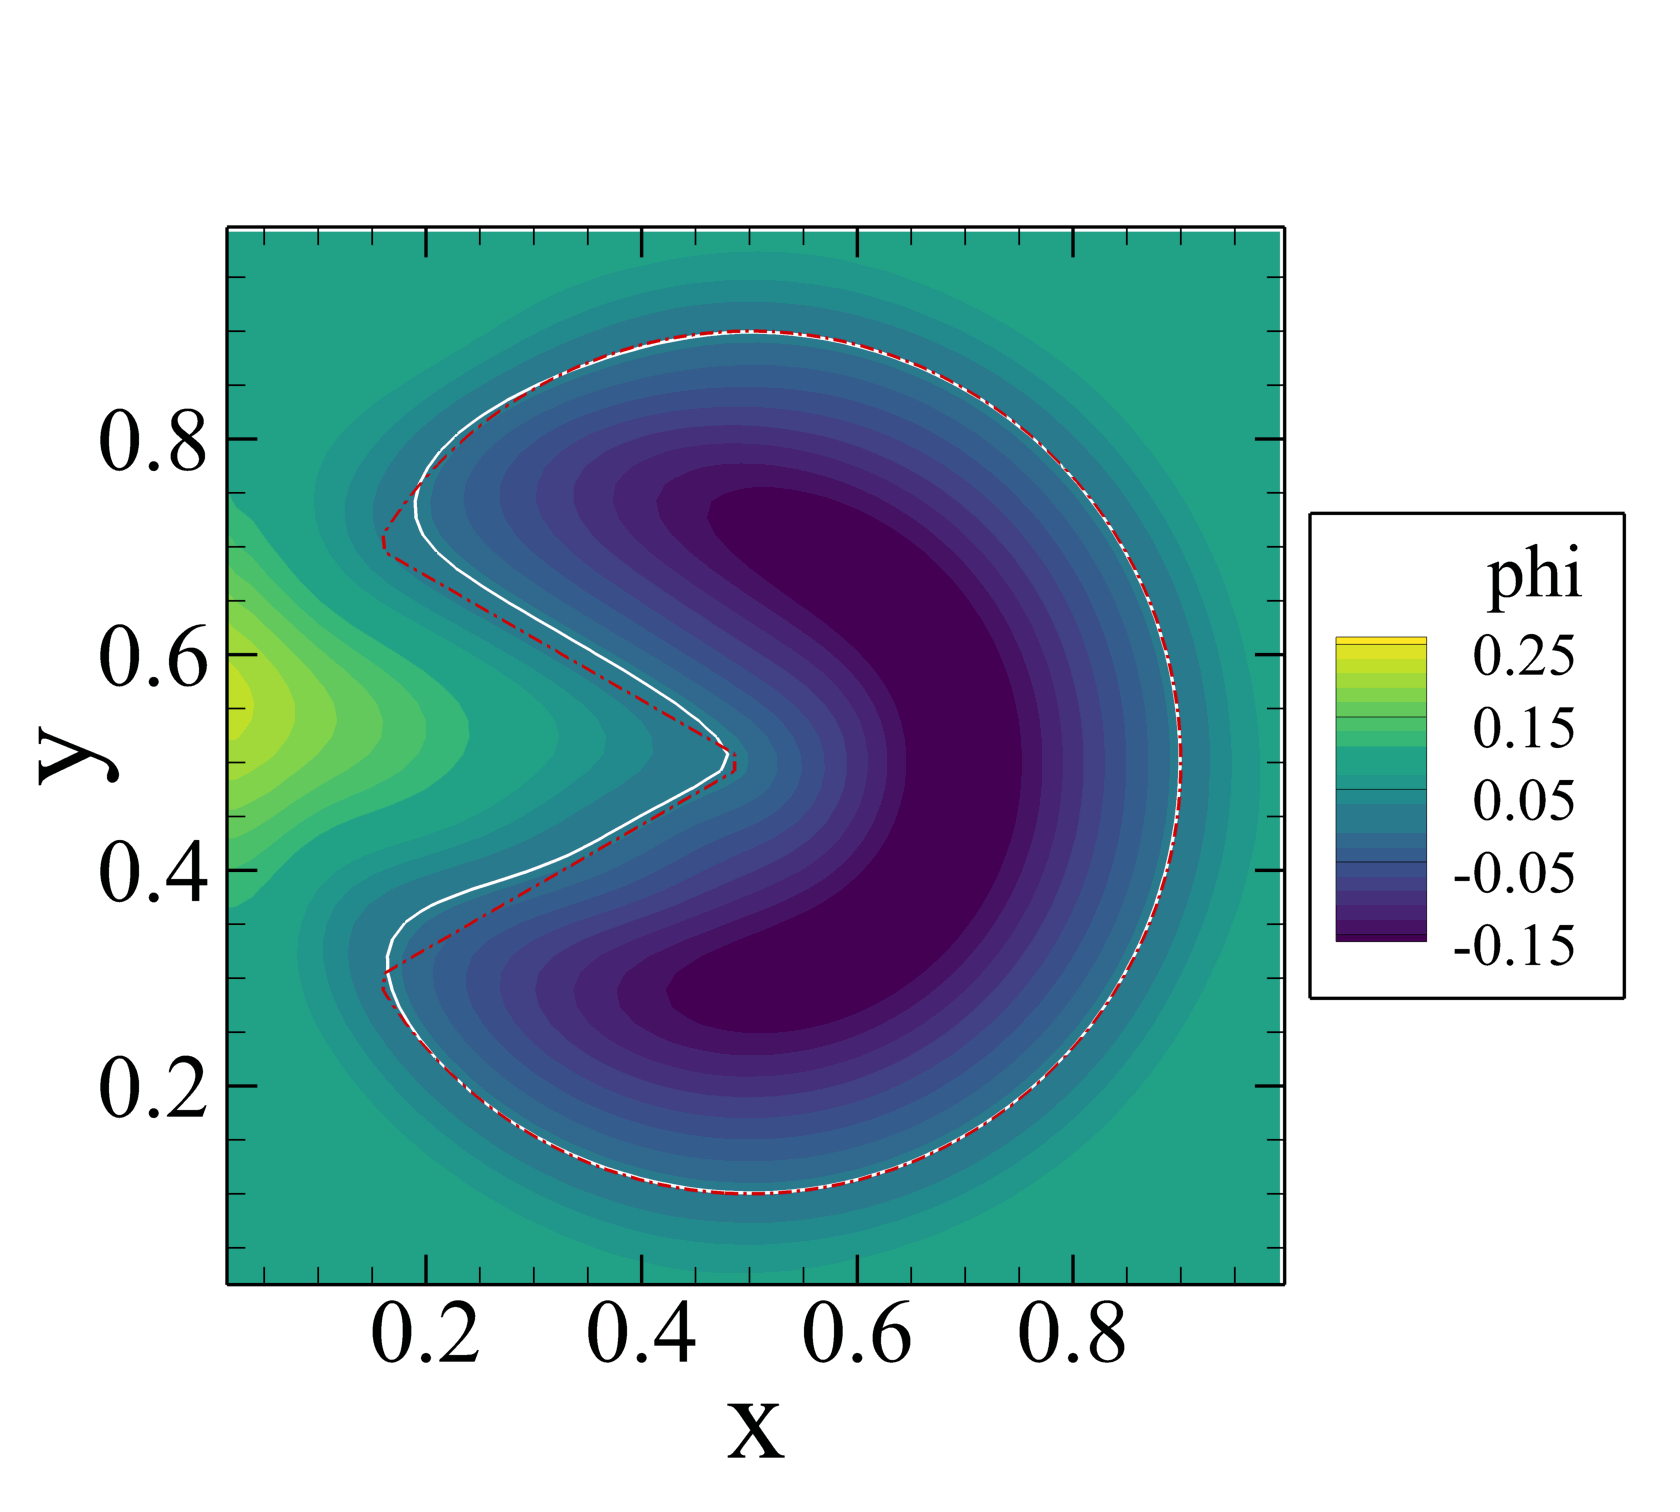
\includegraphics[width=0.4\linewidth]{figure/n64s130t20.png}}
    \subfigure[$128^2$, no reinit]{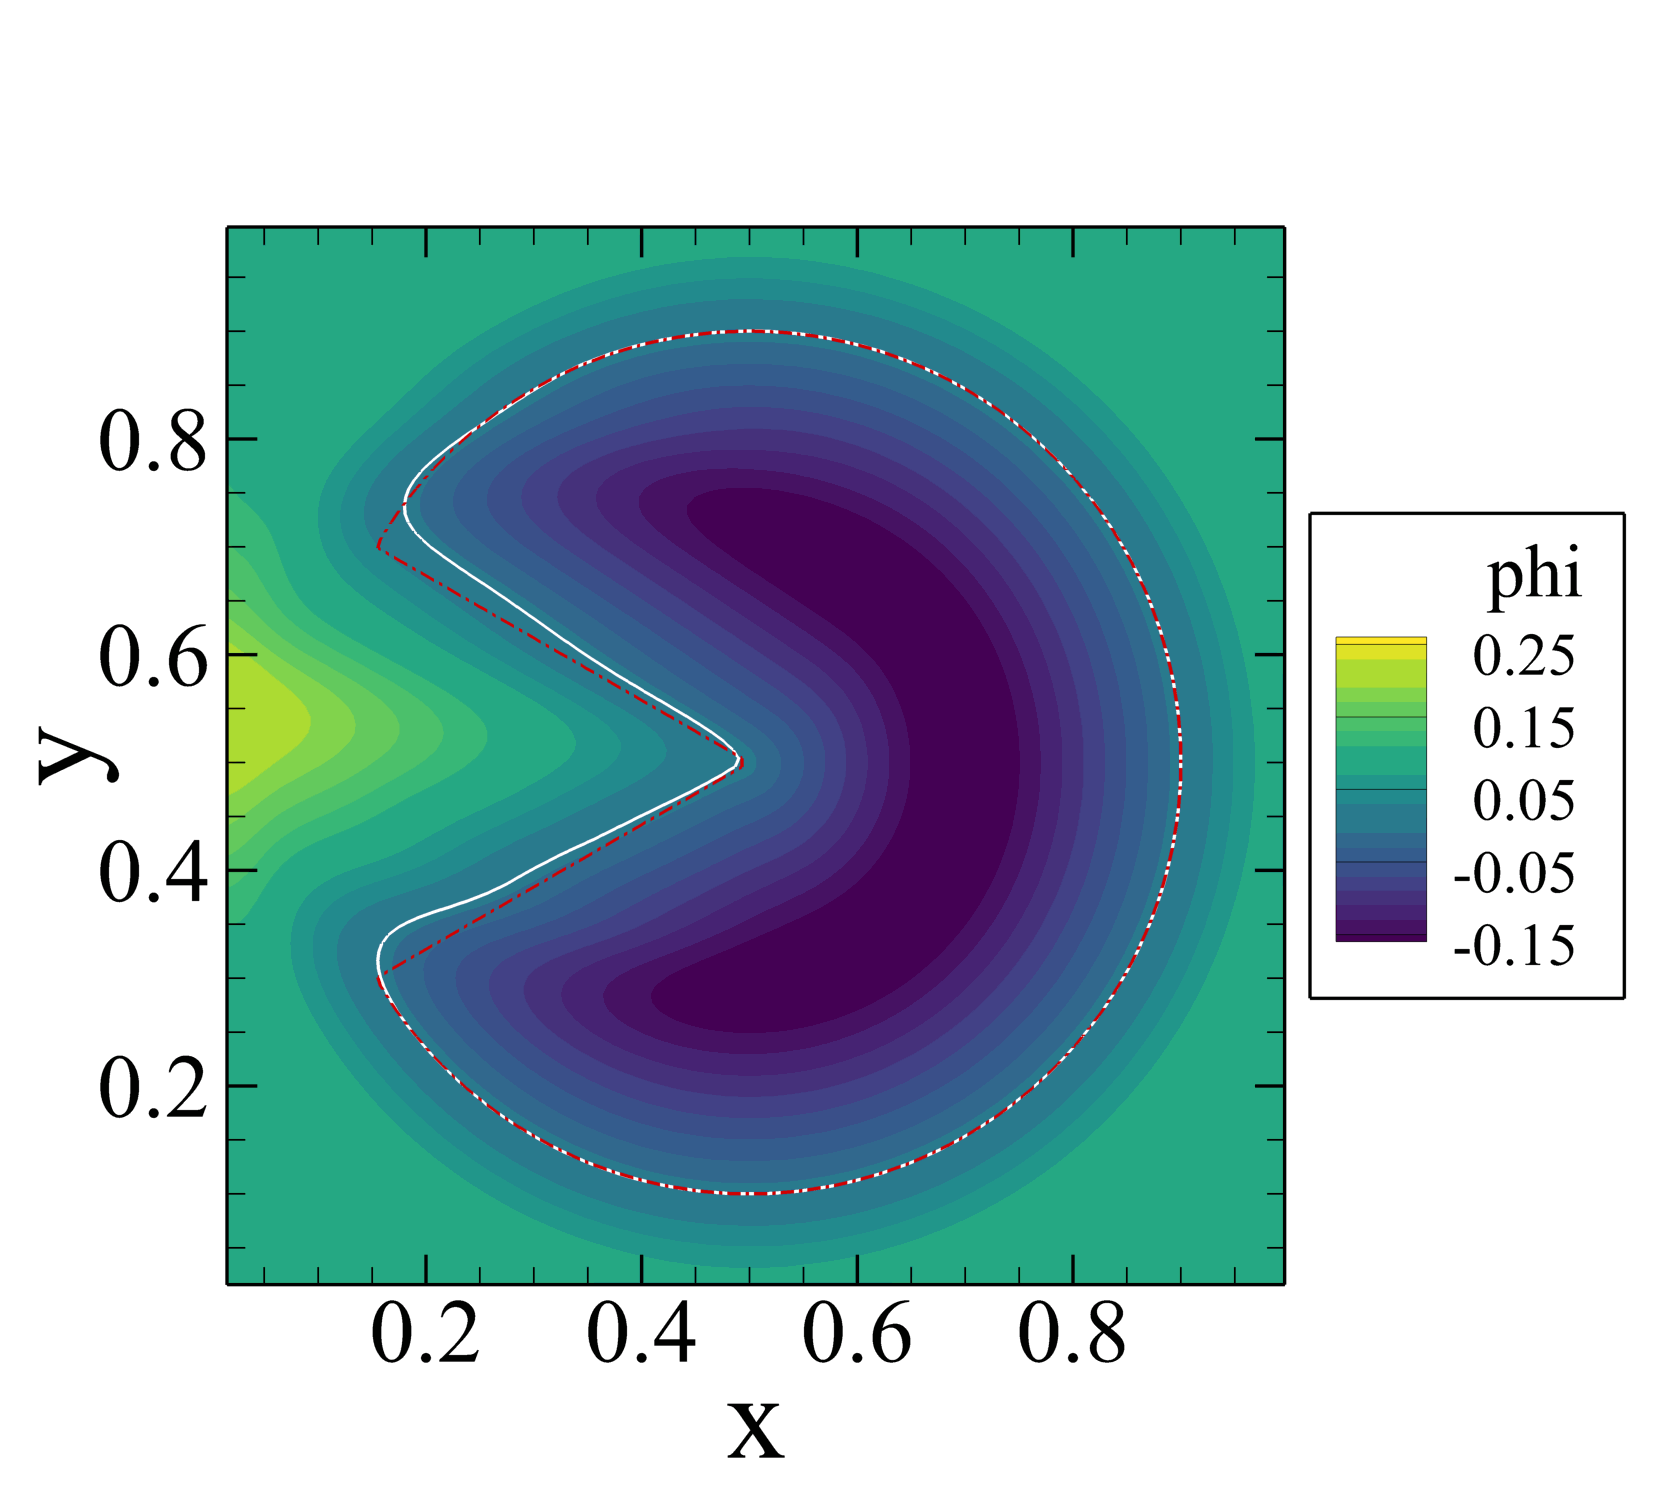
\includegraphics[width=0.4\linewidth]{figure/n128s130t20.png}}
    \subfigure[$64^2$, subcell fix]{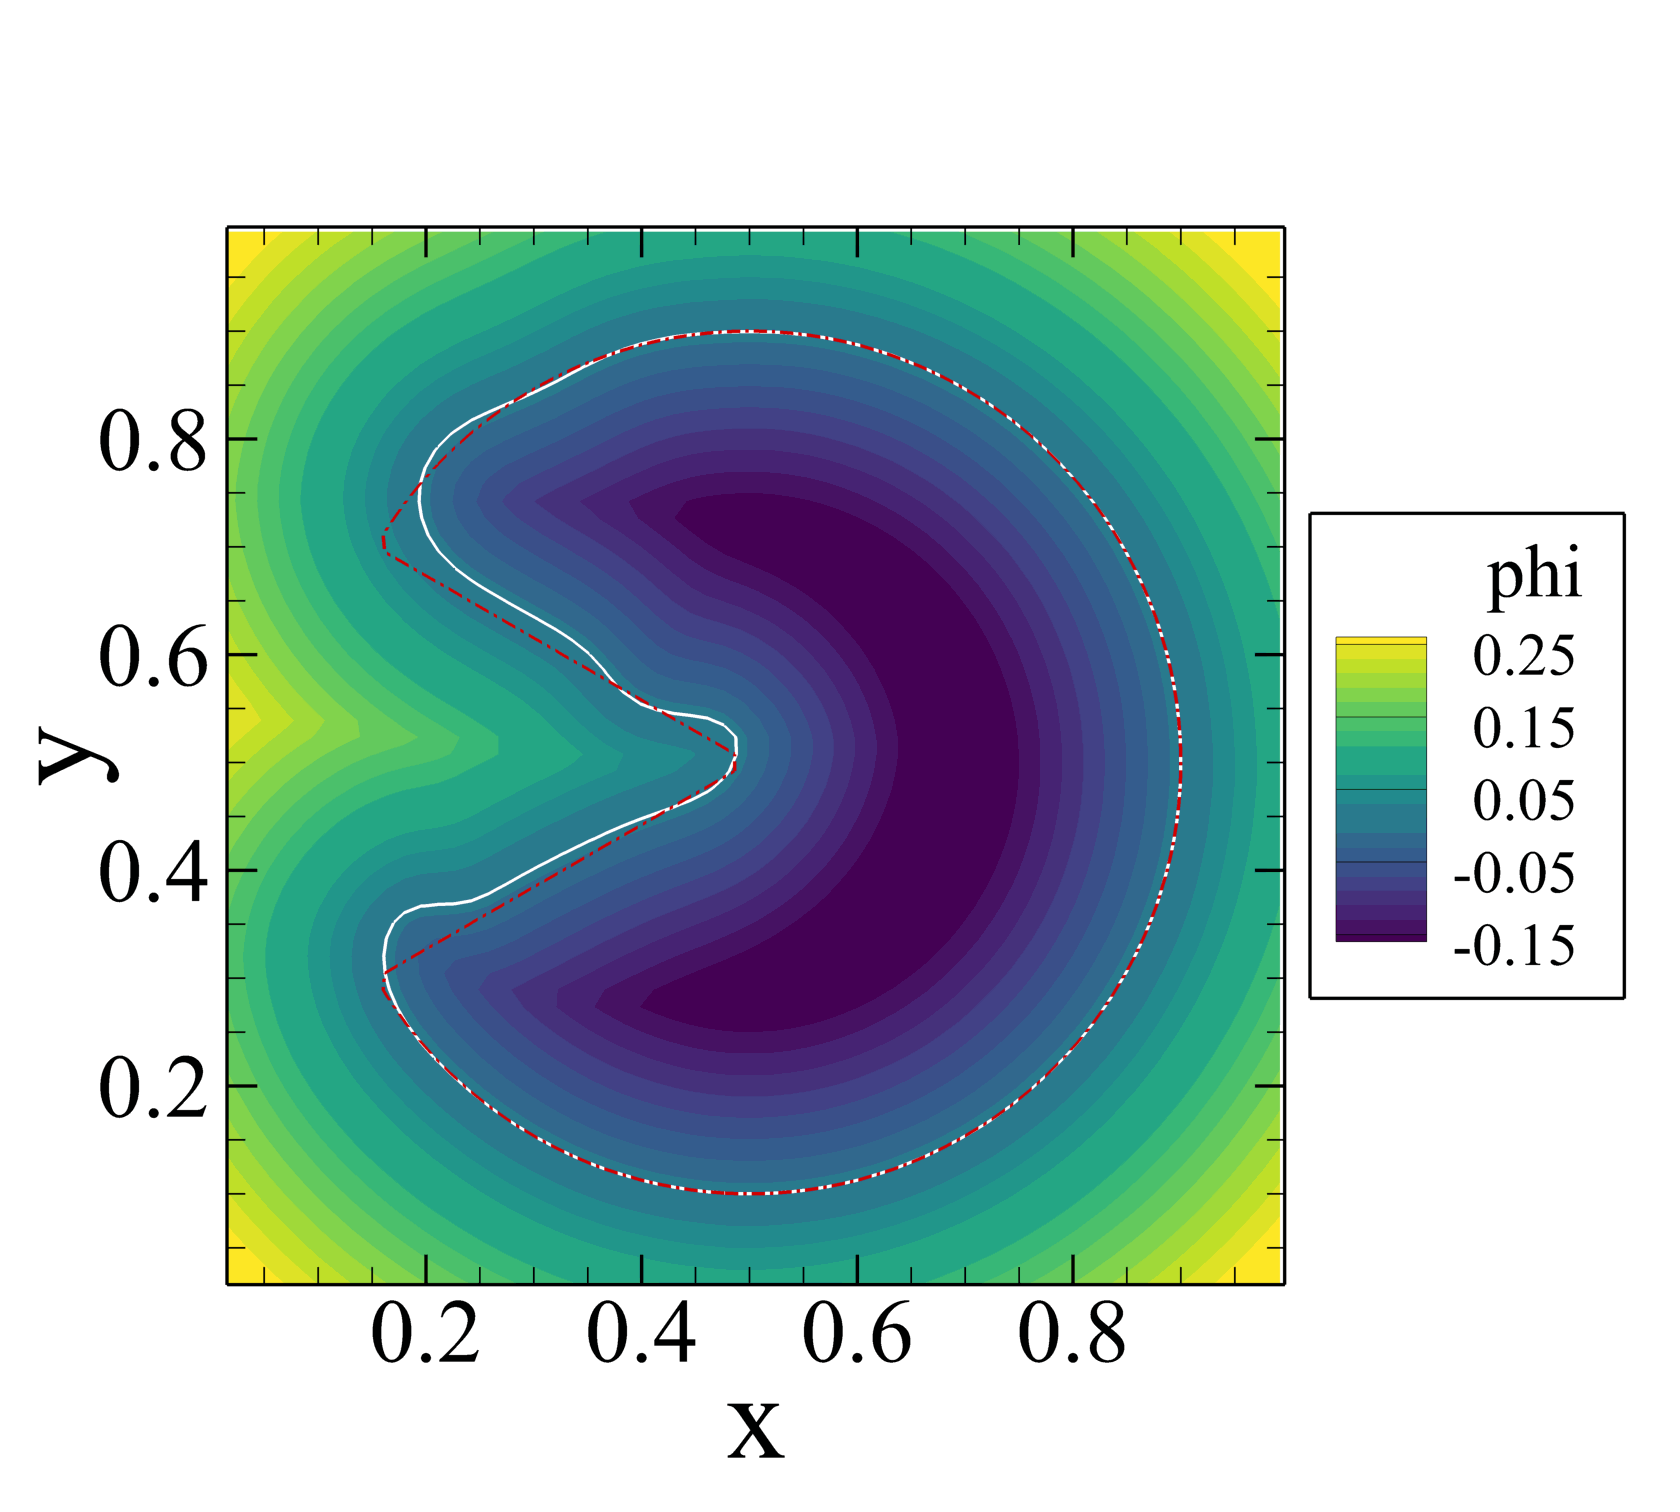
\includegraphics[width=0.4\linewidth]{figure/n64s132t20.png}}
    \subfigure[$128^2$, subcell fix]{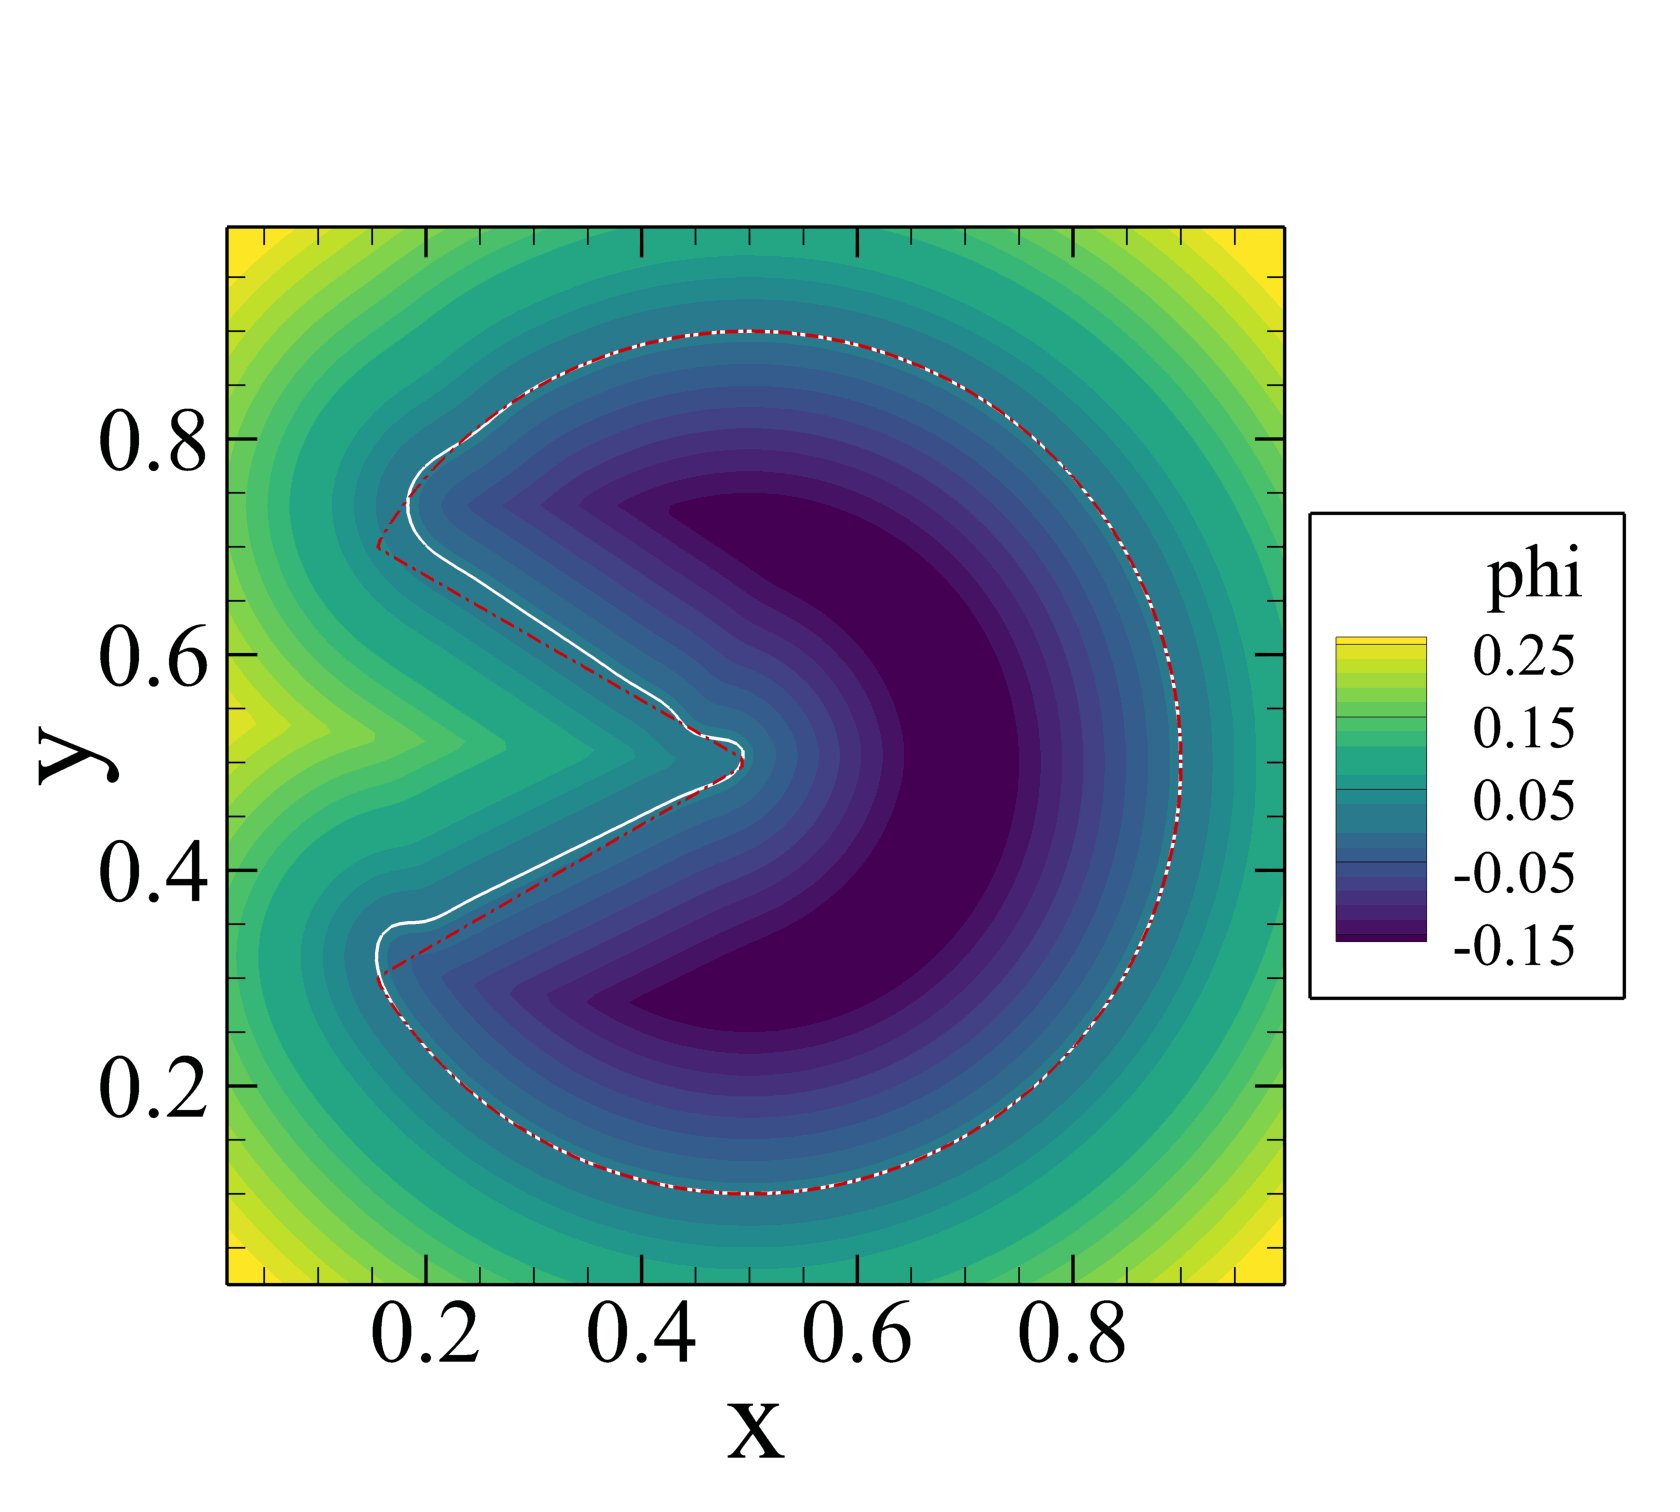
\includegraphics[width=0.4\linewidth]{figure/n128s132t20.png}}
    \subfigure[$256^2$, subcell fix]{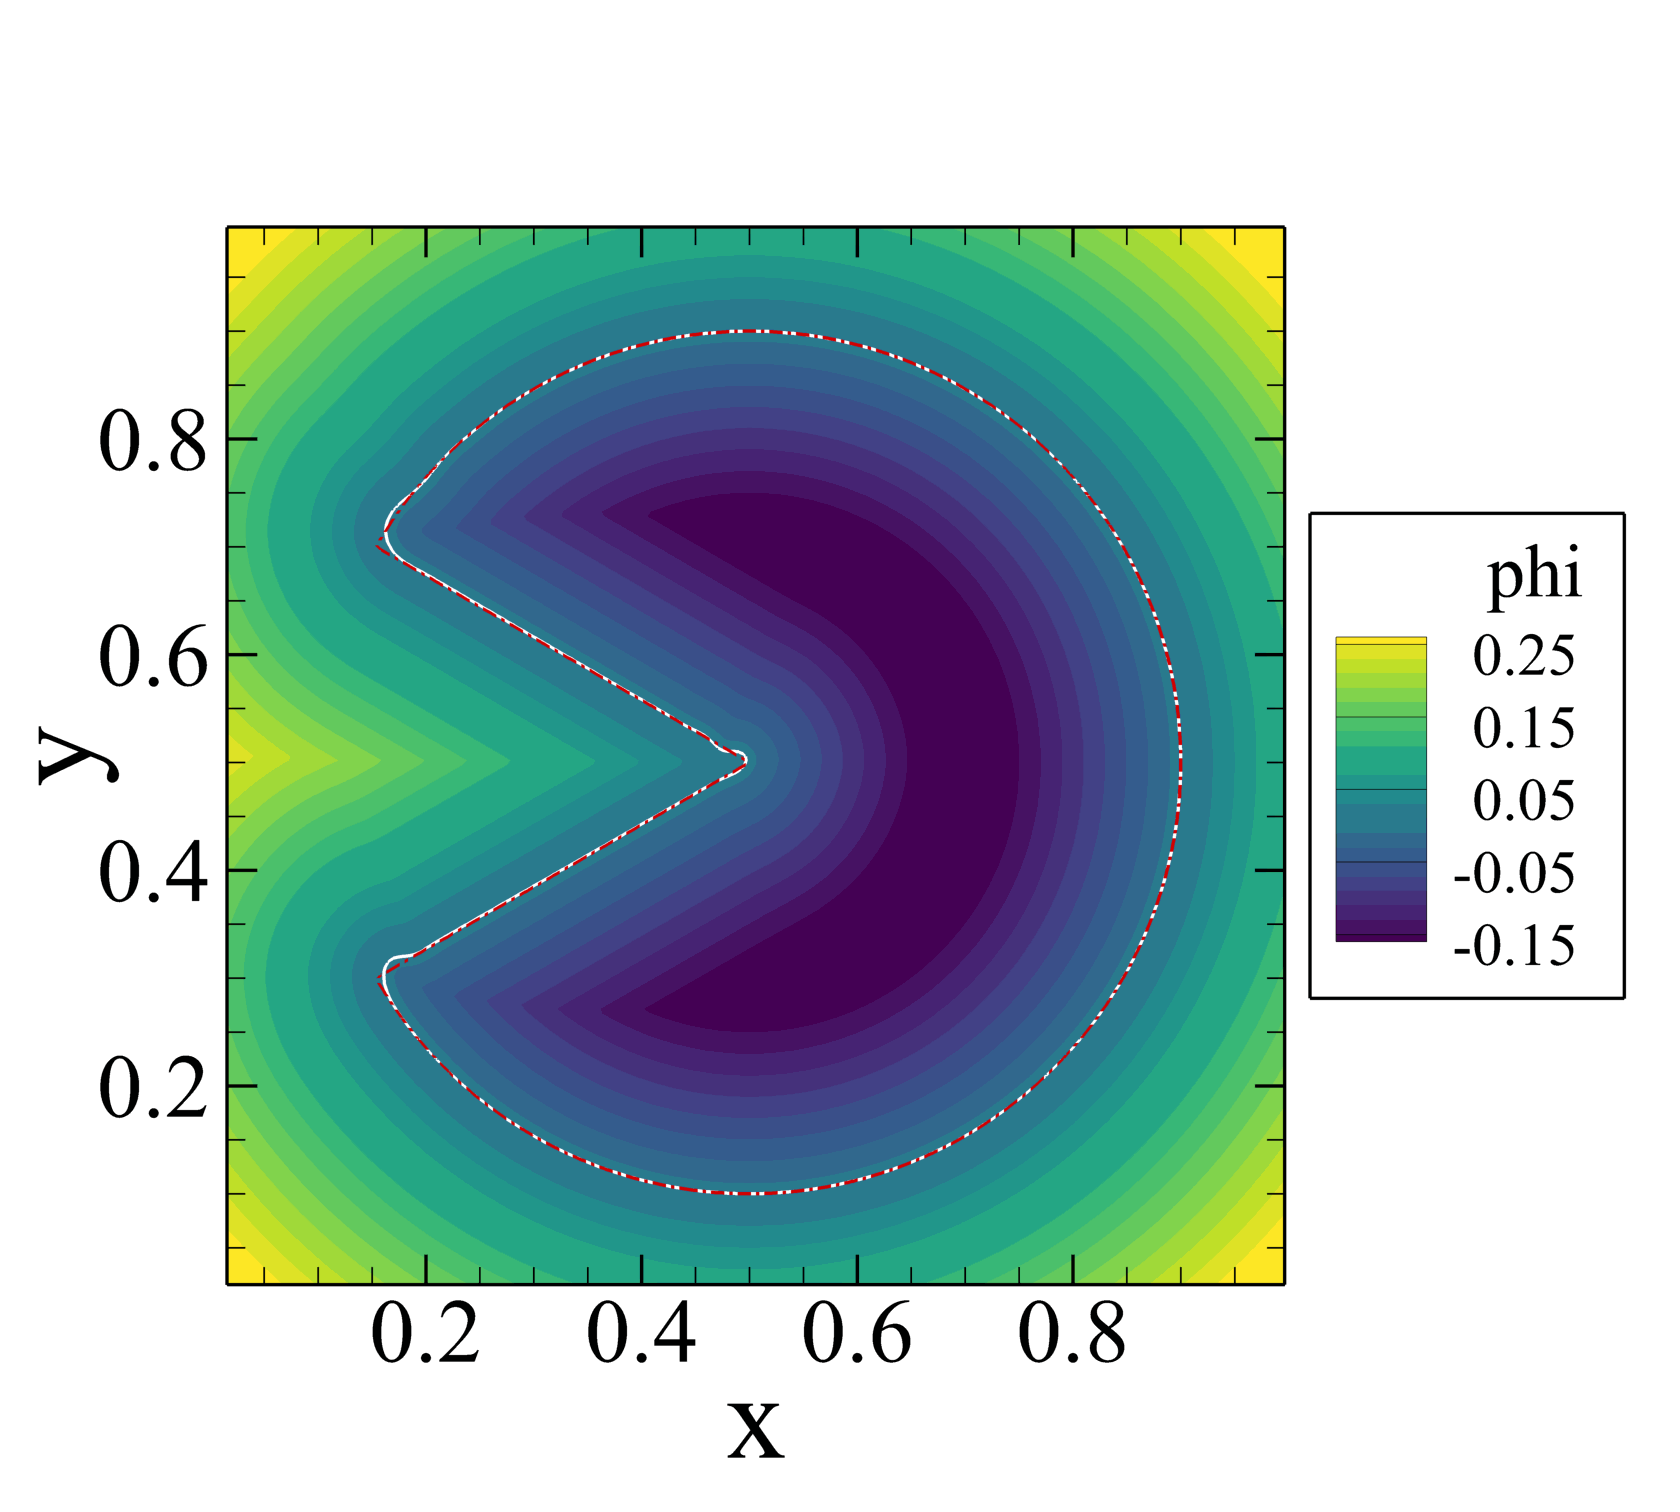
\includegraphics[width=0.4\linewidth]{figure/n256s132t20.png}}
    \subfigure[$512^2$, subcell fix]{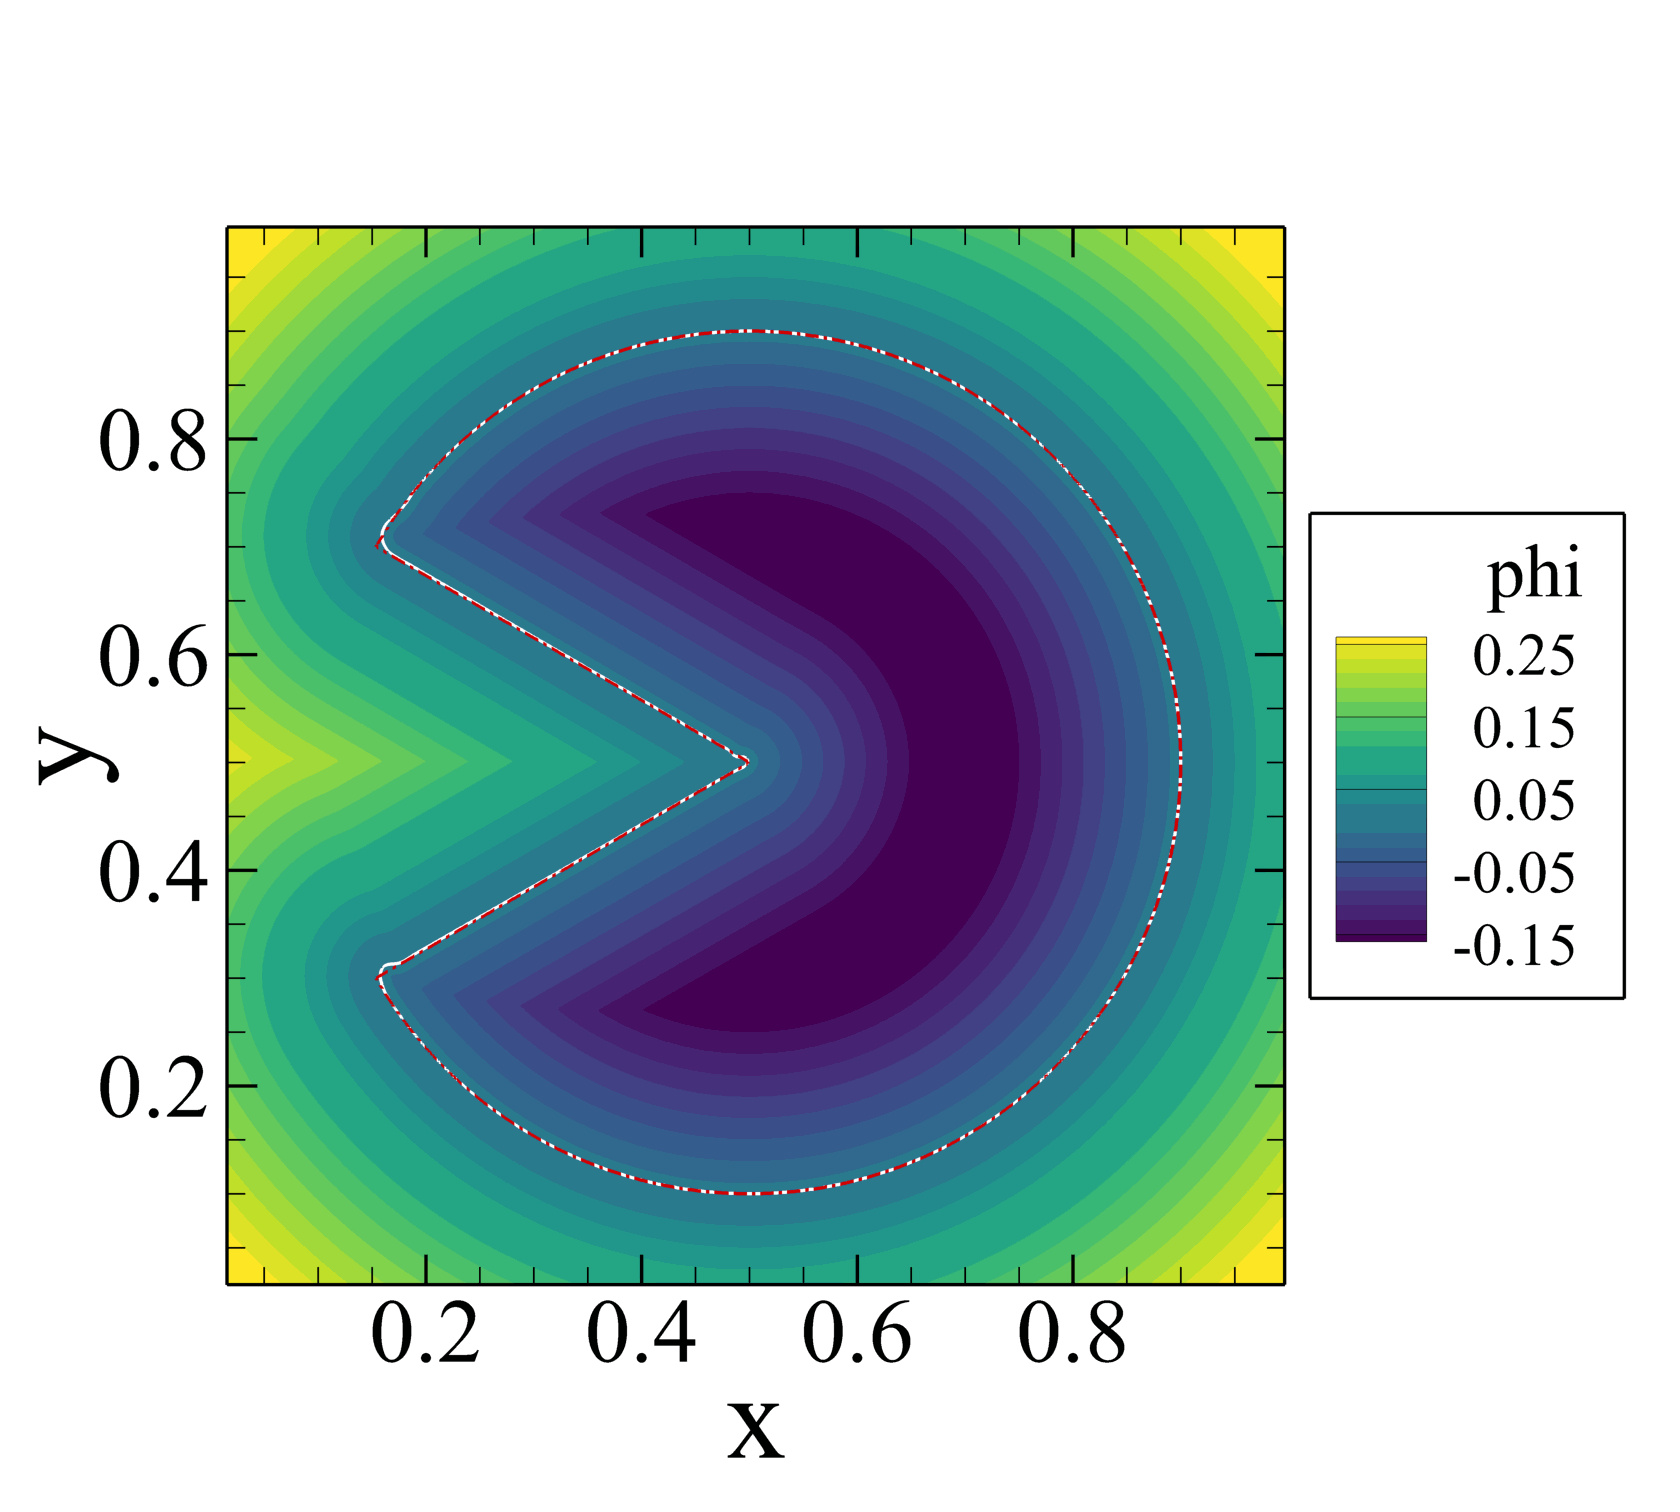
\includegraphics[width=0.4\linewidth]{figure/n512s132t20.png}}
    \caption{\label{fig:rotation}旋转两周($t_\mathrm{max}=2$)后缺角圆盘界面变形情况,红色点划线为初始时刻界面,白色实线为终止时刻界面。}
\end{figure}

\subsection{代码实现简述}
采用c++编写实现了Level Set界面捕捉方法,可以在给定速度场中求解界面演化情况。采用自己编写的数组、交错网格类(class Array, class ArrayStarggered)存储界面函数及流场速度分布,包含自定义的虚拟网格。
\subsubsection{数值格式}
\begin{itemize}
    \item 空间离散格式采用3阶精度的QUICK格式;虚拟网格(ghost nodes)通过直接外推(赋值)或线性外推两种方法计算,由于远离界面处符号距离函数分布对于计算影响不大,通常采用直接赋值以避免数值振荡。
    \item 时间推进实现了forward Euler、TVD-RK2、TVD-RK3三种方法,分别具有1、2、3阶精度,采用后两种方法可以显著提高数值稳定性,进而大幅提高计算效率。
    \item 重新初始化部分实现了\citet{sussman_level_1994}的简单重新初始化方法和\citet{russo_remark_2000}的Subcell fix方法,其基本特性通过前述两个算例得到了很好的验证;内迭代过程采用固定CFL数推进,迭代终止准则为达到足够步数或迭代差的L2模小于参考值。
\end{itemize}

\subsubsection{计算效率}
利用旋转缺角圆盘算例初步检验了代码的计算效率,基本参数设置如下\autoref{tab:param}  
\begin{table}[h]
    \centering
    \caption{\label{tab:param}参数设置}
    \begin{tabular}{lllll}
        \toprule
        $t_\mathrm{max}$ & CFL         & 优化等级 & 空间格式 & 时间格式 \\
        \midrule
        $2.0$            & $0.8,\ 2.0$ & O2       & QUICK    & TVD-RK3  \\
        \bottomrule
    \end{tabular}
\end{table}

试验结果见\autoref{tab:time}(CFL数为2时TVD-RK3仍可稳定计算,结果见\autoref{fig:cfl2}),可以看到代码整体具有不错的效率,$512^2$网格量下包含重新初始化步骤,推进到$t=2$仅需2分钟。统计发现程序总体具有$\mathcal{O}(N^3)$的复杂度(\autoref{fig:complex}),$N$为一个方向上的网格量。
\begin{table}[h]
    \centering
    \caption{\label{tab:time}计算效率测试}
    \begin{tabular}{lllr}
        \toprule
        n   & 重新初始化  & CFL & 计算时间(秒) \\
        \midrule
        64  & Subcell fix & 0.8 & 0.291          \\
        128 & Subcell fix & 0.8 & 2.052          \\
        256 & Subcell fix & 0.8 & 14.359         \\
        512 & Subcell fix & 0.8 & 112.655        \\
        \midrule
        64  & 无          & 0.8 & 0.217          \\
        128 & 无          & 0.8 & 1.477          \\
        256 & 无          & 0.8 & 11.348         \\
        512 & 无          & 0.8 & 88.993         \\
        \midrule
        64  & 无          & 2.0 & 0.107          \\
        128 & 无          & 2.0 & 0.681          \\
        256 & 无          & 2.0 & 4.885          \\
        512 & 无          & 2.0 & 37.998         \\
        \bottomrule
    \end{tabular}
\end{table}

\begin{figure}[htbp]
    \centering
    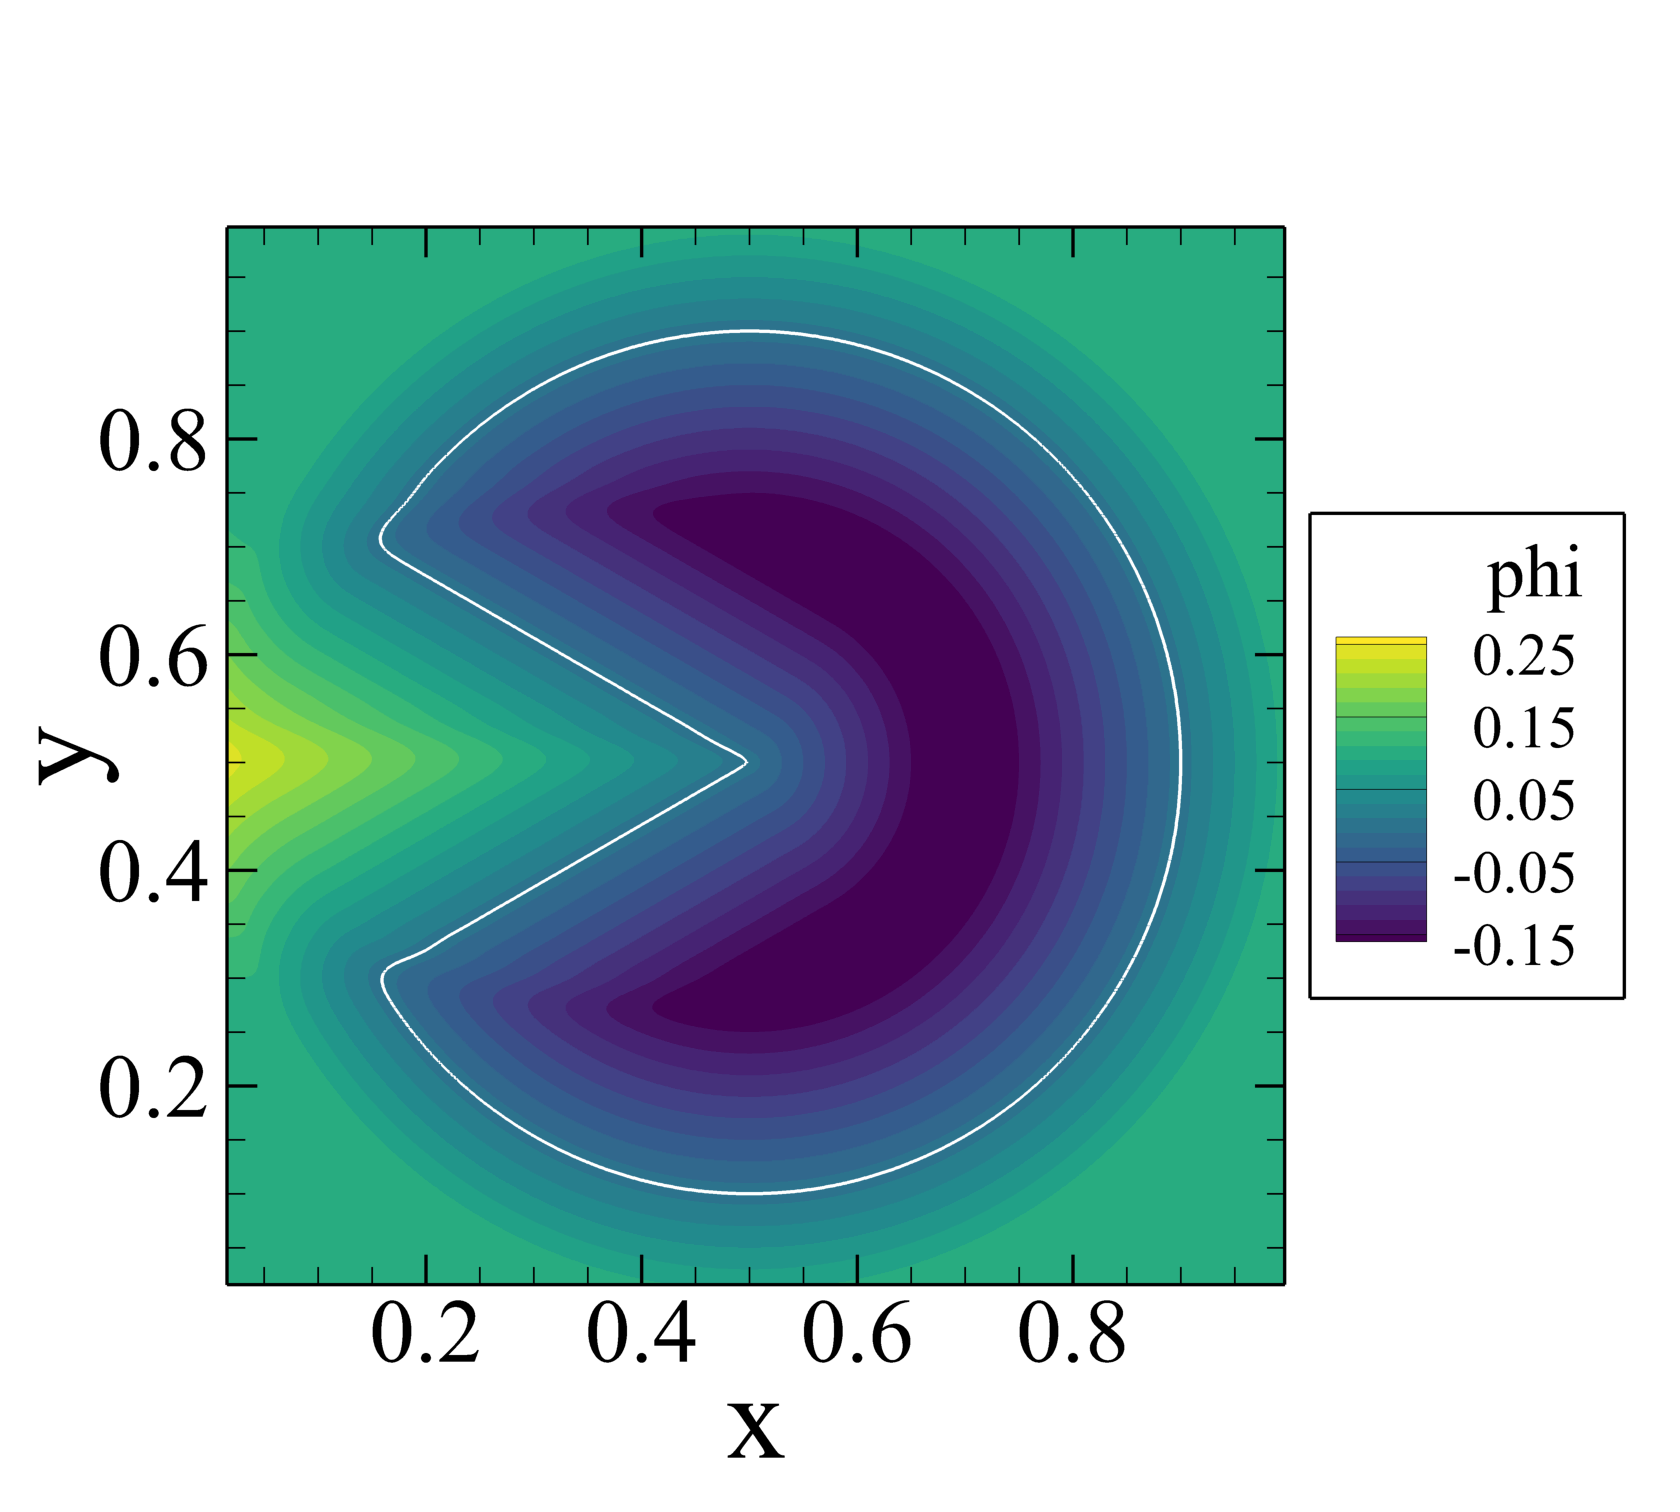
\includegraphics[width=0.6\linewidth]{figure/cfl20n512s130t20.png}
    \caption{\label{fig:cfl2}$512^2$网格,$\text{CFL}=2$,缺角圆盘旋转两周后界面形状及$\phi$云图}
\end{figure}

\begin{figure}[htbp]
    \centering
    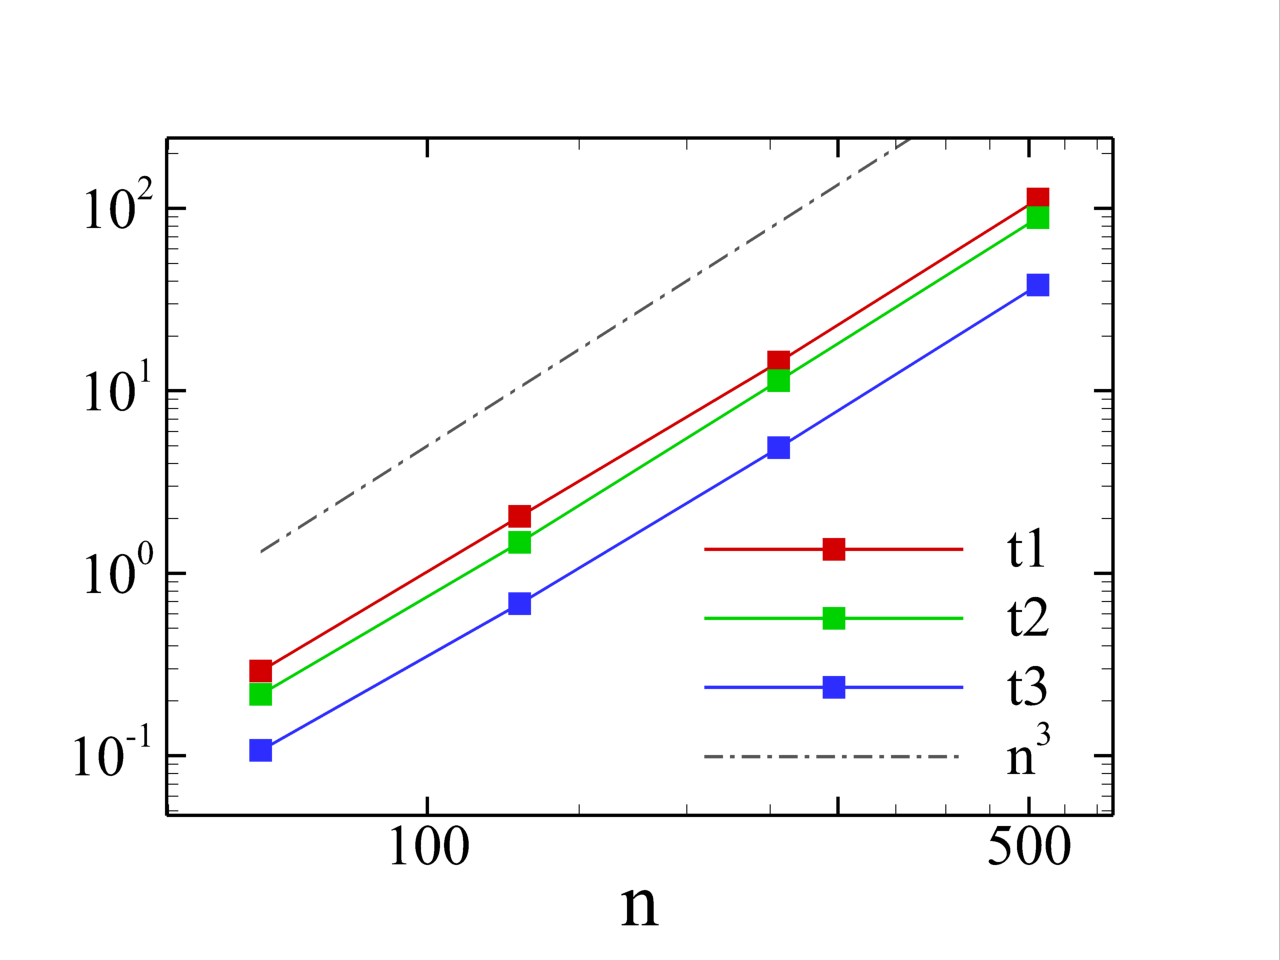
\includegraphics[width=0.6\linewidth]{figure/time.png}
    \caption{\label{fig:complex}程序计算复杂度,三条线分别对应\autoref{tab:time}中三种参数设置}
\end{figure}

\newpage
\bibliographystyle{unsrtnat}
\bibliography{ref}

\end{document}